% !TeX spellcheck = ru_RU
\documentclass[a4paper,12pt,russian]{extarticle}
\usepackage{extsizes}
\usepackage{cmap} % для кодировки шрифтов в pdf
\usepackage[section]{placeins}
\usepackage[T2A]{fontenc}
\usepackage[utf8]{inputenc}
\usepackage[russian]{babel}
\usepackage{slashbox}
\usepackage{graphicx} % для вставки картинок
\graphicspath{ {./figures/} }
\usepackage{amssymb,amsfonts,amsmath,amsthm} % математические дополнения от АМС
\usepackage{indentfirst} % отделять первую строку раздела абзацным отступом тоже
\usepackage[usenames,dvipsnames]{color} % названия цветов
\usepackage{makecell}
\usepackage{csquotes}
\usepackage{multirow} % улучшенное форматирование таблиц
\usepackage{ulem} % подчеркивания
\usepackage{titletoc}
\newtheorem{theorem}{Теорема}


\linespread{1.3} % полуторный интервал
%\renewcommand{\rmdefault}{ftm} % Times New Roman

\fontfamily{ftm}
\frenchspacing


\usepackage[tableposition=top]{caption}
\usepackage{subcaption}
\DeclareCaptionLabelFormat{gostfigure}{Рисунок #2}
\DeclareCaptionLabelFormat{gosttable}{Таблица #2}
\DeclareCaptionLabelSeparator{gost}{~---~}
\captionsetup{labelsep=gost}
\captionsetup[figure]{labelformat=gostfigure}
\captionsetup[table]{labelformat=gosttable}
\renewcommand{\thesubfigure}{\asbuk{subfigure}}

\usepackage[left=3cm,right=1cm,
top=2cm,bottom=2cm,bindingoffset=0cm]{geometry}

\AtBeginDocument{%
	\let\mtcontentsname\contentsname
	\renewcommand\contentsname{\normalsize{\MakeUppercase\mtcontentsname}} %Заголовок содержания капсом
	
	\let\LaTeXStandardTableOfContents\tableofcontents %Убрать жирный шрифт в содержании
	\renewcommand{\tableofcontents}{%
		\begingroup%
		\renewcommand{\bfseries}{\relax}%
		\LaTeXStandardTableOfContents%
		\endgroup%
	}%
}

\usepackage{tikz}
\usepackage{float}
\usetikzlibrary{chains,shapes.multipart}
\usetikzlibrary{shapes,calc}
\usetikzlibrary{automata,positioning}

\begin{document}	
% НАЧАЛО ТИТУЛЬНОГО ЛИСТА
	\begin{center}\linespread{1}
		\hfill \break
		\large{Министерство науки и высшего образования Российской федерации}\\
		\footnotesize{НАЦИОНАЛЬНЫЙ ИССЛЕДОВАТЕЛЬСКИЙ}\\ 
		\footnotesize{ТОМСКИЙ ГОСУДАРСТВЕННЫЙ УНИВЕРСИТЕТ (НИ ТГУ)}\\
		\footnotesize{Институт прикладной математики и компьютерных наук}\\
		\footnotesize{Кафедра прикладной информатики}\\
		\hfill\break
		\hfill \break
		\hfill \break
	\end{center}
\begin{flushright}\linespread{0.9}
	\normalsize{ДОПУСТИТЬ К ЗАЩИТЕ В ГЭК}\\ 
	\hfill \break
	\normalsize{ 
			Зав.каф. прикладной информатики\\  д-р.физ.-мат.н.,  профессор\\ \underline{\hspace{2cm}} Е.М. Семёнов\\
			\textquote{\underline{\hspace{0.7cm}}}\underline{\hspace{2cm}}2021 г.		
	}\\
\end{flushright}
\hfill \break
\hfill \break
\begin{center}\linespread{1}
		\large\textbf{ БАКАЛАВРСКАЯ РАБОТА}\\
		\hfill \break
		\large{ИССЛЕДОВАНИЕ ДВУМЕРНОГО ВЫХОДЯЩЕГО ПОТОКА МАРКОВСКОЙ МОДЕЛИ УЗЛА ОБРАБОТКИ ЗАПРОСОВ С ПОВТОРНЫМИ ОБРАЩЕНИЯМИ И ВЫЗЫВАЕМЫМИ ЗАЯВКАМИ}\\
		\hfill \break
		\hfill \break
		\normalsize{по основной образовательной программе подготовки бакалавров\\
			направление  подготовки\\
			090303 - Прикладная информатика\\
		\hfill \break
	Благинин Алексей Леонидович}\\
		\hfill \break
		\hfill \break
	\end{center}
\begin{flushright}\linespread{0.9}
	\normalsize{ 
		Руководитель ВКР\\
		 доцент.каф. прикладной информатики\\ \underline{\hspace{2cm}} И.Л. Лапатин\\
		 \textquote{\underline{\hspace{0.7cm}}}\underline{\hspace{2cm}}2021 г.\\
		 \hfill \break
		  Автор работы\\
		  студент группы № 931704\\ \underline{\hspace{2cm}} А.Л. Благинин	
	}\\
\end{flushright}
	\hfill \break
	\hfill \break
	\begin{center} Томск-2021 \end{center}
	\thispagestyle{empty} % выключаем отображение номера для этой страницы
	\clearpage
	% КОНЕЦ ТИТУЛЬНОГО ЛИСТА % Титульный лист
\section*{\normalsize\centering АННОТАЦИЯ}
Работа содержит \pageref{LastPage} страниц, \totalfigures\ рисунков, \totaltables\ таблицы, 67 источников.
 
ТЕОРИЯ МАССОВОГО ОБСЛУЖИВАНИЯ, СИСТЕМА МАССОВОГО ОБСЛУЖИВАНИЯ С ПОВТОРНЫМИ ВЫЗОВАМИ И ВЫЗЫВАЕМЫМИ ЗАЯВКАМИ, МЕТОД АСИМПТОТИЧЕСКОГО АНАЛИЗА, ИМИТАЦИОННОЕ МОДЕЛИРОВАНИЕ.

Объект исследования: оптимизация проведения численных экспериментов для систем теории массового обслуживания.
Методы исследования: метод имитационного моделирования, метод асимптотического анализа. 

Результаты работы: имитационное моделирование было рассмотрено как численный метод исследования систем массового обслуживания. Был спроектирован и реализован программный комплекс с набором инструментов для анализа систем теории массового обслуживания, содержащий имитационную модель, алгоритмы вычисления характеристик и вспомогательные утилиты. Был предложен метод обращения характеристических функций на основе дискретного преобразования Фурье для эффективного вычисления асимптотических результатов. На ряде примеров был проиллюстрирован подход к работе с программным комплексом и задачи, которые он позволяет решать.

Актуальность данной работы обусловлена универсальностью метода численного исследования систем, так как он может выступать и в качестве  отдельной методологии исследования, так и позволяет подтверждать имеющие аналитические результаты и делать косвенные выводы об аспектах работы системы, которые еще не были получены аналитически, но доступны к изучению численно. Для получения достоверных численных результатов в большинстве задач требуется проведение большого числа экспериментов при различных параметрах системы. Работа посвящена оптимизации процесса проведения численных экспериментов в условиях ограниченных вычислительных ресурсов и времени.

В первом разделе описан метод моделирования систем массового обслуживания и алгоритм для его проведения. Во второй главе описана архитектура, процесс разработки и особенности реализации программного комплекса. В третьей главе описаны подходы к обращению характеристических функций для работы с асимптотическими результатами исследования моделей. В четвертой главе описывается процесс работы с реализованным программным комплексом на примере исследования модели RQ---системы с повторными вызовами и обратной связью методами машинного обучения, где в качестве обучающей выборки выступают результаты имитационного моделирования.

\thispagestyle{empty}\addtocounter{page}{-1} % выключаем отображение номера для этой страницы
\clearpage

\begin{center}
\tableofcontents % Содержание 
\clearpage
\end{center}

\section {Введение}
Многие ситуации с очередями имеют особенность, заключающуюся в том, что клиенты, обнаруживающие, что зона обслуживания занята по прибытии, должны временно покинуть ее и присоединиться к группе неудовлетворенных клиентов, но они повторяют свой запрос через некоторое случайное время. Говорят, что между испытаниями заказчик находится на орбите. Эти модели массового обслуживания возникают при стохастическом моделировании многих протоколов связи, локальных сетей и повседневных жизненных ситуаций. Самый простой и очевидный пример - это человек, который звонит по телефону. Если линия занята, значит, он не может стоять в очереди, но через некоторое время снова испытывает удачу. Для систематического изложения основных методов и основных результатов по этой теме мы отсылаем читателя к книгам [1], [2] и библиографической информации, приведенной в [3], [4], [5]. Чтобы проиллюстрировать активную роль очередей на повторное рассмотрение за последние несколько лет, упомянем некоторые недавние статьи, опубликованные в этом журнале [6], [7], [8], [9], [10], [11], [12] ].

В большинстве публикаций, посвященных очередям повторного запроса, сервер обслуживает только тех, кто поступает от постоянных клиентов. Однако существуют реальные ситуации (например, сценарий call-центра), когда серверы имеют возможность совершать исходящие телефонные звонки, когда они не участвуют в разговоре. Эта функция организации очереди известна как парная коммутация или модели двусторонней связи. В ранней литературе Фалин [13] вывел интегральные формулы для частичных производящих функций и явные выражения для ожидаемого значения некоторых характеристик производительности очереди повторных вызовов с двухсторонней связью в предположении, что длительности входящих и исходящих вызовов соответствуют одинаковым распределение времени обслуживания. Однако на практике это предположение носит ограничительный характер, поскольку разные типы клиентов обычно демонстрируют разное поведение и, следовательно, у них должны быть разные потребности в обслуживании. Арталехо и Ресинг [14] использовали метод анализа среднего значения для получения некоторых ожидаемых значений, связанных со временем ожидания в очереди на повторное обращение с двусторонней связью и различным распределением времени обслуживания входящих и исходящих вызовов. Недавно Artalejo и Phung-Duc [15] провели подробное исследование очереди на повторное рассмотрение с двухсторонней связью. Полученные результаты включают явные выражения для совместного стационарного распределения состояния сервера и количества заявок на орбите, а также для частичных факториальных моментов. Большинство явных формул в [15] выражены в терминах гипергеометрических рядов, что согласуется с той особой ролью, которую играют эти специальные функции при выводе аналитических решений для многих других очередей повторных попыток [16], [17], [18] , [19], [20], [21].

Наша главная цель в этой статье - дать представление об исследовании очередей повторного запроса на одном сервере с двусторонней связью. С этой целью мы сначала проводим тщательное исследование очереди повторного запроса -типа с различным распределением времени входящего и исходящего обслуживания. Для этой модели получены как стационарные, так и асимптотические результаты. Стационарный анализ основан на хорошо известных математических инструментах, но они предоставляют новые выражения в замкнутой форме и стабильные вычислительные схемы для производительности системы. Таким образом, мы надеемся, что наши явные формулы будут полезны в приложениях. С другой стороны, асимптотический подход, используемый в этой статье, подразумевает заметное алгебраическое упрощение по сравнению с выводами, необходимыми для получения аналоговых асимптотических результатов для классической очереди повторных вызовов (без исходящих вызовов) [22]. Еще одна цель этой статьи - использовать марковский процесс прибытия (MAP) и распределение типа фазы (PH) для создания более сложных очередей повторных запросов с двусторонней связью, допускающей неэкспоненциальные прибытия и корреляцию между временами прибытия.





782 ИИСУС Р. АРТАЛЕХО И ТУАН ПХУНГ-ДУК
В последнее время большое внимание уделяется очередям на повторное рассмотрение, потому что они
иметь приложения для анализа производительности различных систем, таких как центры обработки вызовов,
компьютерные сети и телекоммуникационные системы [3, 12, 17, 28]. Очереди на повторное рассмотрение
характеризуются тем, что клиенты (т.е. звонки), которые не могут получить услугу
по прибытии выйдите на виртуальную орбиту и повторите попытку обслуживания через некоторое случайное время.
Поток прибытия с орбиты делает нижележащую марковскую цепочку очередей на повторное рассмотрение
быть неоднородным. В результате анализ очередей на повторное рассмотрение намного сложнее.
чем у соответствующих моделей массового обслуживания без повторных попыток и явных результатов
получаются лишь в некоторых частных случаях [3, 12, 23, 24].
Гипергеометрические функции и их специальные версии играют важную роль в
вывод аналитических решений для очередей на повторное рассмотрение. Фактически стационарный
характеристики состояния системы обычной очереди повторных запросов M / M / 1/1
выражается через специальные гипергеометрические функции [3, 12, 24]. Обзор
2000 Математическая классификация предметов. Первичный: 68М20, 90Б22; Вторичный: 60К25.
Ключевые слова и фразы. Очереди повторных вызовов, двусторонняя связь, смешанные центры обработки вызовов, стационарное распределение, факторные моменты, рекурсивные формулы, асимптотический анализ.
Рецензированием статьи занимались Уи Юэ и Ютака Такахаши в качестве гостя.
Редакторы.
существующая литература показывает, что гипергеометрические функции также являются ключевым инструментом для
анализировать стационарные характеристики (т.е. предельные вероятности состояния системы
и их частичные производящие функции) широкого спектра очередей повторных попыток, включая
одиночные серверные очереди с отказом Бернулли [12, 24], очереди на повторное рассмотрение M / M / 1/1
тип с отказом Бернулли и обратной связью [9], очереди повторных запросов на одном сервере с
орбитальный поиск и непостоянные заявки [19], очередь повторных запросов M / M / 1/1 с
линейная политика повторного рассмотрения [2] и очередь повторного рассмотрения M / M / 2/2 [14]. Может быть, последний
пример принадлежит Киму [16], который изучает очередь повторных запросов на одном сервере с конфликтом
и нетерпение при использовании гипергеометрических функций.
В большинстве публикаций по очередям повторного вызова сервер обслуживает только входящие вызовы.
После обслуживания вызова сервер ждет либо следующего поступления основного вызова, либо
для повторного вызова. Однако бывают ситуации из реальной жизни, когда у серверов есть
возможность совершать исходящие телефонные звонки. Наиболее очевидное применение возникает в повседневной
жизнь, потому что каждый использует телефонную линию или мобильный телефон для приема звонков, но
также для звонков на улицу. Более того, в различных системах обслуживания, таких как звонок
центр, оператор не только обслуживает входящие звонки, но и совершает исходящие звонки.
звонит, если он свободен. Пока сервер занят, входящие звонки не могут
получить услугу. Мы предполагаем, что эти вызовы присоединяются к орбите, и снова пытаемся занять
сервер после некоторого экспоненциально распределенного времени независимо от других вызовов.
В настоящее время бизнес колл-центра очень важен, потому что он обеспечивает канал
для двусторонней связи между компаниями и их клиентами [1, 18, 26].
Как правило, существует два типа центров обработки вызовов: центры обработки вызовов для входящих и исходящих вызовов.
Первый используется для поддержки клиентов, когда клиенты звонят извне для некоторых
такие запросы, как бронирование билетов и подтверждение данных кредитной карты
или жалоба на продукцию и т. д. [27]. С другой стороны, последний используется для
телефонный маркетинг, при котором система набора номера случайным образом направляет
призывы к потенциальным клиентам для рекламы или продажи новых продуктов [26]. Недавно,
современные центры обработки вызовов объединяют как входящие, так и исходящие функции, чтобы увеличить
продуктивность [7, 10]. Они называются смешанными центрами обработки вызовов, в которых оператор
не только принимает входящие звонки, но и звонит клиентам, когда он или
она простаивает.
Бхулаи и Кул [7] предлагают модель организации массового обслуживания с несколькими серверами с бесконечным буфером для
смешанные центры обработки вызовов, для которых разработаны оптимальные и почти оптимальные политики для
случай, когда входящие и исходящие вызовы имеют одинаковое экспоненциальное распределение
и в противном случае соответственно. Deslauriers et al. [10] разработать пять марковских очередей
модели смешанных центров обработки вызовов, в которых различаются входящие и исходящие вызовы
и незаметно. Как указано в [10], модели входящего и
исходящие вызовы с разными распределениями сложнее, чем с
одинаковое распределение времени обслуживания для обоих типов вызовов. В этих работах [7, 10]
повторные испытания не учитываются.
Фалин [11] выводит интегральные формулы для частичных производящих функций и явные выражения для некоторых ожидаемых показателей эффективности повторного испытания M / G / 1/1.
очередь с двусторонней связью, в которой входящие и исходящие вызовы
предполагается, что они следуют тому же распределению услуг. Choi et al. [8] расширяют модель Фалина
в очереди повторного вызова M / G / 1 / K, где входящие и исходящие вызовы также предполагается
следуйте тому же распределению времени обслуживания. Однако с точки зрения приложения
точки зрения, это предположение носит ограничительный характер, поскольку входящие и исходящие вызовы могут
имеют разное распределение времени обслуживания. Арталехо и Ресинг [5] получают первые
ПОВТОРНЫЕ ОЧЕРЕДИ С ДВУСТОРОННЕЙ СВЯЗЬЮ 783
частичные моменты для очереди повторных вызовов M / G / 1/1 с различным распределением времени обслуживания входящих и исходящих вызовов с использованием подхода анализа среднего значения. Это
Следует отметить, что анализ среднего значения не может использоваться для получения стационарного
распределения, а также высшие факторные моменты.
В этом документе термин двухсторонняя связь относится к тому факту, что сервер
может совершать исходящие звонки, пока не участвует в разговоре. Есть
ряд моделей повторного судебного разбирательства, которые связаны с этим определением двухстороннего
коммуникационная функция. Фактически, с аналитической точки зрения, два пути
модель коммуникации можно даже рассматривать как частный случай других существующих
модели, которые по своему происхождению были разработаны для моделирования других различных очередей
Особенности. Это случай ссылок [21, 6, 12].
Мартин и Арталехо [21] рассматривают очередь M / G / 1/1 с двумя типами нетерпеливых
единицы, которые можно рассматривать как очередь на повторное рассмотрение с двусторонней связью. В [21] a
заблокированный заказчик хранится в орбитальной очереди, из которой только заказчик
Глава очереди может повторить попытку после экспоненциально распределенного времени. Авраченков
и другие. [6] использовать методы матричного анализа для изучения очереди повторных запросов на одном сервере с
два класса клиентов, чьи повторные попытки и распределения времени обслуживания
разные. Прибытие происходит в соответствии с ярко выраженным марковским процессом прибытия.
Несомненно, что рассмотрение обобщенных марковских приходов, допускающих
корреляция - интересная цель. Однако следует отметить, что методика
использованный в [6] не дает явных решений. Фалин и Темплтон [12] представляют
предварительный анализ многоклассовых очередей на повторное рассмотрение M / G / 1/1, для которых система
представлены уравнения для среднего числа заявок на орбите. В
авторы в [12] также указывают на некоторые открытые проблемы для модели, которые требуют дальнейшего
изучение.
Существующая библиография по очередям на повторное рассмотрение обширна и обширна. В результате в
В дополнение к вышеупомянутым ссылкам можно было бы найти другие повторные судебные разбирательства
модели, относящиеся к двухсторонней очереди связи, исследуемой здесь. В целом,
среди ближайших вариантов повторного исследования отметим мультикласс, приоритетный и нетерпеливый
повторные модели. Для общего обзора читатель отсылается к разделу 2.3 в
Artalejo и Gomez-Corral [3], а также к обновленной библиографии [4].
Первая и основная цель этой статьи - предоставить более обширный анализ
очереди на повторное рассмотрение M / M / 1/1 с двухсторонней связью и другим сервисом
временное распределение входящих и исходящих звонков. В частности, мы предоставляем явные
решения для совместного стационарного распределения состояния сервера и
количество заявок на орбите, частные факториальные моменты и их порождающие
функции. Мы также приводим рекурсивные формулы для стационарного распределения и
частные факториальные моменты, на основе которых как символьные, так и численные алгоритмы
могут быть реализованы. Кроме того, мы выводим несколько простых асимптотических формул для
стационарное распределение и частные факториальные моменты.
Вторая цель этой статьи - обсудить расширение мультисерверного повторного тестирования.
очереди с двусторонней связью и различным распределением входящих и исходящих вызовов, для которых мы получаем некоторые явные результаты. В частности, мы устанавливаем
необходимое и достаточное условие устойчивости системы и вывести явную формулу для среднего количества входящих вызовов на серверах. Кроме того, мы
Сформулируйте мультисерверную модель с помощью зависимой от уровня квазиворождения и смерти (QBD)
процесс, который может быть использован для численного исследования. Надеемся, что наша модель
полезен для анализа производительности смешанных центров обработки вызовов.
784 ИИСУС Р. АРТАЛЕХО И ТУАН ПХУНГ-ДУК
Оставшаяся часть теста организована следующим образом. Раздел 2 описывает модель в
деталь. Раздел 3 посвящен основным результатам данной статьи, в которой обширный
представлено исследование очереди повторных попыток M / M / 1/1 с двусторонней связью.
В разделе 4 мы обсуждаем расширение многосерверной очереди повторных запросов с двухсторонней
общение и получить некоторые явные результаты. 


СТАТЬЯ
В этой статье мы рассматриваем двумерный процесс вывода системы массового обслуживания.
[6,8] с повторными вызовами [1] и вызванными приложениями [7]. Такую систему можно интерпретировать
как узел обработки с множественным произвольным доступом, который в свободное время
обработки запросов может запросить самодиагностику или любую другую процедуру, которая
будет продолжаться в случайное время. Также может применяться рассматриваемая система
для моделирования узлов обработки с разными типами приложений. Приложения
одного вида не теряются и обслуживаются в любом случае, а заявки
другой тип будет обслуживаться только с бесплатным ресурсом.
Отдельные узлы образуют модель сети связи, в которой
исходящий поток из одного узла входит в другой. В случае приложений
разных типов, после обслуживания на определенном узле, они уходят по своим маршрутам.
Таким образом, результаты исследования выходных процессов систем массового обслуживания
широко применяются для проектирования реальных систем передачи данных и
анализ сложных процессов, состоящих из нескольких этапов. В связи с этим для
2 А.Благинин, И.Лапатин
моделируя сети, важно иметь информацию о наличии
корреляция между процессами в нем. Слабая корреляция позволяет
рассматривать процессы как независимые при моделировании, что может существенно
упростить модель и ее исследование.
В данной работе мы рассматриваем влияние параметров системы на
значения асимптотического коэффициента корреляции компонент двумерной
процесс вывода разных типов приложений. Чтобы изучить систему,
метод асимптотического анализа используется для нахождения вида предельного
двумерное распределение количества обслуженных заявок ввода
процесс и количество обслуженных вызванных заявок за некоторое время t, при условии
что на орбите наблюдается большая задержка заявок [10].

КУРСАЧ
Человек, в своей повседневной жизни, постоянно сталкивается с необходимостью получить доступ к различным ресурсам, к которым пытаются получить доступ и другие люди. При этом ресурсы могут быть совершенно разной природы – касса в магазине, консультация преподавателя, место в общественном транспорте и многие другие. Во всех этих случаях человек чаще всего сталкивается с очередью, которая может быть как упорядоченной, так и неупорядоченной.
Математическим моделированием и изучением закономерностей, возникающих при различных способах организации доступа к ресурсу, занимается теория массового обслуживания [1]. Заметим, что англоязычное название (queuing theory) на русский язык переводится как теория очередей. [2] Теория массового обслуживания возникла еще в начале ХХ века. А.К. Эрланг [3], решая практические задачи совершенствования работы систем связи, получил рад формул, которые являются базовыми для теории массового обслуживания. Терминология, используемая в теории массового обслуживания, соответствует исходным задачам – заявка, прибор, требование, буфер и другие.
Классическими моделями массового обслуживания являются модели с очередью и модели с отказами. В моделях с очередью заявка (требование), которая обратилась к прибору (ресурсу) и застала его занятым, встает в очередь для ожидания обслуживания. В моделях с отказами заявка при невозможности получить обслуживание теряется. Существует достаточно много модификаций и комбинаций таких моделей. 
Во второй половине ХХ века происходит бурное развитие телекоммуникационных сетей, что приводит к необходимости моделировать и проектировать сети передачи данных различной структуры и назначения. Для этого стали применяться модели систем массового обслуживания с повторными вызовами. В системах такого типа заявка, которая не может получить доступ к ресурсу повторяет попытку захвата ресурса через случайную задержку, а не встает в очередь. В англоязычной литературе такие модели называются retrial queue (RQ), большой обзор работ по исследованию которых приведен в монографии [4].
Заметим, что большинство работ посвящены исследованию характеристик состояния самой системы (число заявок в системе, среднее время пребывания в системе) [5, 6], а исследованию выходящих потоков уделяется недостаточно внимания. При этом, в разного рода системах обслуживания, таких как системы телекоммуникационной связи, автоматизированные call-центры, компьютерные сети и др., одной из важнейших и представляющей большой практический интерес характеристик является именно число обслуженных заявок, то есть выходящий поток заявок.
Исследование выходящих потоков усложнятся тем, что его характеристики зависят от функционирования самой системы. Это увеличивает размерность задачи и далеко не всегда делает возможным получить решение аналитически. Результаты для выходящих потоков классических систем были получены еще в середине ХХ века [7, 8]. Обзор работ по исследованию выходящих потоком содержится в [9]. В работе [9] рассматриваются выходящие потоки систем с повторными вызовами.
Качественное и структурное изменение реальных систем требует разработки новых математических моделей, которые позволят точно описывать их функционирование. В данной работе предлагается исследовать выходящий поток системы с повторными вызовами и вызываемыми заявками.
Такую систему можно интерпретировать как узел сети связи со случайным множественным доступом, который в свободное от обработки запросов время может запросить самодиагностику или другую процедуру, которая будет продолжаться случайное время. Так же модель call-центра, в которой вызываемые заявки могут интерпретироваться как «холодные звонки» клиентам, в то время, как линия не занята.
Отдельные узлы образуют модель сети связи, в которой выходящий поток одного узла является входящим для другого, поэтому результаты исследования выходящих потоков сетей массового обслуживания широко применимы для проектирования реальных систем передачи данных и анализа сложных процессов, состоящих из нескольких этапов.


 \clearpage %Введение
\titleformat{\section}[block]
{\normalsize\bfseries\hspace{\parindent}}
{\thesection}
{1em}{}
\section {Исследование систем с простейшим входящим потоком}
В этом разделе предлагаются к рассмотрению системы с повторными вызовами и вызываемыми заявками, заявки в которые приходят посредством простейшего (Пуассоновского) потока.\\
Рассмотрим общий вид RQ--системы с простейшим входящим потоком:\\
 На вход поступает простейший поток заявок с интенсивностью $\lambda$. Заявка входящего потока, поступая в систему и обнаруживая прибор свободным, занимает его. Прибор, в свою очередь, начинает обслуживание в течение случайного времени, распределенного экспоненциально с параметром $\mu_{1}$. Если же при поступлении в систему заявка обнаруживает прибор занятым, она мгновенно уходит на орбиту и осуществляет там случайную задержу в течение экспоненциально распределенного времени с параметром $\sigma$. В свободное от обслуживания заявок с входящего потока время прибор сам вызывает заявки с интенсивностью $\alpha$ и обслуживает их в течение экспоненциально--распределенного времени с параметром $\mu_{2}$.
\begin{figure}[H]
	\centering
	\includegraphics[scale=0.5]{common_model.eps}
	\caption{Общий вид RQ--системы с простейшим входящим потоком}
	\label{common_model_fig}
\end{figure}
Введем следующие обозначения: $i(t)$ --- число заявок на орбите в момент времени $t$, $k(t)$ --- состояние прибора: $0$ --- прибор свободен, $1$ --- прибор занят обслуживанием заявки входящего потока, $2$ --- прибор занят обслуживанием вызванной заявки. 
 
Поскольку целью исследования является характеристика работы выходящего потока системы, будет рассмотрено два варианта предложенной модели --- с суммарным и двумерным выходящими потоками.
\subsection{RQ-система с суммарным выходящим потоком}
Суммарный выходящий поток RQ-системы подразумевает, что приходящие заявки и заявки, вызываемые прибором самостоятельно, являются однородными, посему результат работы системы рассматривается как совокупность обслуженных заявок входящего потока и вызванных. 
\begin{figure}[H]
	\centering
	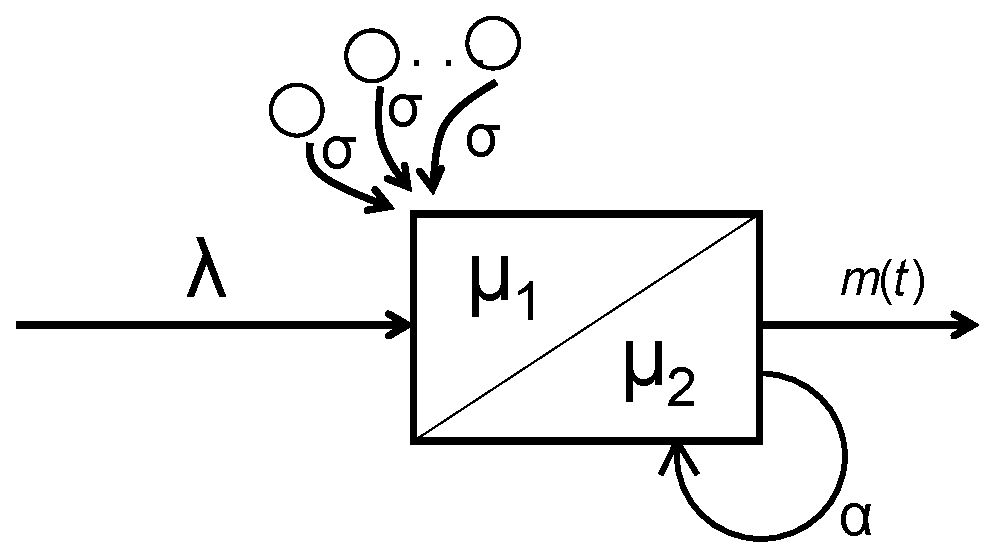
\includegraphics[scale=0.5]{summary_output_model.eps}
	\caption{Модель RQ-системы с суммарным выходящим потоком}
	\label{summary_output_model_fig}
\end{figure}
Введем обозначение: $m_(t)$ — число обслуженных заявок в момент времени $t$.


\subsubsection{Уравнения Колмогорова}
Итак, мы имеем три характеристики, определяющие результат функционирования системы за некоторое время $t$: состояние прибора – $k(t)$, количество заявок на орбите – $i(t)$ и количество обслуженных заявок – $m(t)$, что можно представить в виде трехмерного Марковского процесса
\begin{equation*}
	\{k(t),i(t),m(t)\}
\end{equation*}
Заметим, что именно такая комбинация характеристик будет являться Марковским процессом, так как даёт достаточно информации о том, какое состояние система примет в следующий момент времени. Для этого необходимо знать, в каком состоянии прибор был в предшествующий момент времени, и какое количество заявок находилось в источнике повторных вызовов.
Следующее состояние, которое прибор может принять, зависит от состояния, в котором он находился прежде, то есть, каждое из трех состояний $k(t)$ принимается прибором с некоторыми вероятностями. Введем их в рассмотрение
\begin{equation*}
	\begin{split}
		P\{k(t)=0,i(t)=i,m(t)=m\} &=P_{0}(i,m,t)\\
		P\{k(t)=1,i(t)=i,m(t)=m\} &=P_{1}(i,m,t)\\
		P\{k(t)=2,i(t)=i,m(t)=m\} &=P_{2}(i,m,t)
	\end{split}
\end{equation*}
Теперь, необходимо определить вероятность перехода в каждое из трех состояний. Для этого обратимся к модели и рассмотрим $k(t) = 0$, то есть, состояние, в котором прибор свободен. Чтобы в следующий момент времени $t+\Delta t$ прибор был свободен необходимо выполнение одного из следующих условий:
\begin{enumerate}
	\item Прибор был свободным в момент времени $t$ и к моменту времени $t+\Delta t$  прибор не вызвал заявку, не пришла заявка с входящего потока и не было обращений заявок с орбиты.
	\item На момент времени $t+\Delta t$ прибор закончил обслуживание заявки с входящего потока.
	\item На момент времени $t+\Delta t$ прибор закончил обслуживание вызываемой заявки.
\end{enumerate}
Таким образом, применяя формулу полной вероятности, вероятность того, что прибор окажется свободен в момент времени $t+\Delta t$ равна сумме вероятностей наступления вышеперечисленных условий:
\begin{equation*}
	P_{0}(i,m,t+\Delta t)=P_{0}(i,m,t)(1-\alpha\Delta t)(1 - i\sigma\Delta t)(1-\lambda\Delta t)+P_{1}(i,m-1,t)\mu_{1}\Delta t + P_{2}(i,m-1,t)\mu_{2}\Delta t
\end{equation*}
Аналогично для принятия состояния, в котором прибор занят, необходимо выполнение одного из следующих условий:
\begin{enumerate}
	\item Прибор был занят в момент времени $t$,  и к моменту времени $t+\Delta t$ прибор не закончил обслуживание заявки, и не пришла заявка с входящего потока.
	\item Прибор был свободен, и пришла заявка с входящего потока.
	\item Прибор был свободен, и повторно обратилась заявка с орбиты.
	\item Прибор был занят, и пришла заявка с входящего потока, сразу переместившись на орбиту.
\end{enumerate}
В результате получим следующее равенство:
\begin{equation*}
	\begin{split}
			P_{1}(i,m,t+\Delta t)&=P_{1}(i,m,t)(1-\lambda\Delta t)(1-\mu_{1}\lambda\Delta t)+P_{0}(i,m,t)\lambda\Delta t +\\ &+ P_{0}(i+1,m,t)(i+1)\sigma\Delta t + P_{1}(i-1,m,t)\lambda\Delta t + o(t)
	\end{split}
\end{equation*}
Вероятность принятия прибором состояния обслуживания вызываемой заявки является суммой следующих вероятностей:
\begin{enumerate}
	\item Прибор обслуживал вызываемую заявку, и к моменту времени $t+\Delta t$ прибор не закончил обслуживание вызываемой заявки, и не пришла заявка с входящего потока.
	\item Прибор обслуживал вызываемую заявку, и пришла заявка с входящего потока. Поскольку прибор занят, она ушла на орбиту.
	\item Прибор был свободен, и он вызвал заявку.
\end{enumerate}
Получим равенство:
\begin{equation*}
	P_{2}(i,m,t+\Delta t)=P_{2}(i,m,t)(1-\alpha\Delta t)(1 - \lambda\Delta t)(1 - \mu_{2}\Delta t)+P_{2}(i-1,m,t)\lambda\Delta t + P_{0}(i,m,t)\alpha\Delta t + o(t)
\end{equation*}
Запишем получившуюся систему уравнений
\begin{equation*} 
	\begin{split}
		P_{0}(i,m,t+\Delta t)&=P_{0}(i,m,t)(1-\alpha\Delta t)(1 - i\sigma\Delta t)(1-\lambda\Delta t) +\\ &+ P_{1}(i,m-1,t)\mu_{1}\Delta t + P_{2}(i,m-1,t)\mu_{2}\Delta t,
		\\
		P_{1}(i,m,t+\Delta t)&=P_{1}(i,m,t)(1-\lambda\Delta t)(1-\mu_{1}\lambda\Delta t)+P_{0}(i,m,t)\lambda\Delta t +\\ &+ P_{0}(i+1,m,t)(i+1)\sigma\Delta t + P_{1}(i-1,m,t)\lambda\Delta t + o(t),
		\\
		P_{2}(i,m,t+\Delta t)&=P_{2}(i,m,t)(1-\alpha\Delta t)(1 - \lambda\Delta t)(1 - \mu_{2}\Delta t) +\\ &+ P_{2}(i-1,m,t)\lambda\Delta t + P_{0}(i,m,t)\alpha\Delta t + o(t).
	\end{split}
\end{equation*}
Так как почти все слагаемые содержат $\Delta t$, разделим систему на $\Delta t$ и сделаем предельный переход $\Delta t \rightarrow 0$

\begin{equation} \label{kolmogorov_equations_summary}
	\begin{split}
		\frac{{\partial P_{0}(i,m,t)}}{{\partial t}} &= -(\lambda + i\sigma + \alpha)P_{0}(i,m,t) + P_{1}(i,m-1,t)\mu_{1} + P_{2}(i,m-1,t)\mu_{2},
		\\
		\frac{{\partial P_{1}(i,m,t)}}{{\partial t}} &= -(\lambda + \mu_{1})P_{1}(i,m,t) + (i+1)\sigma P_{0}(i+1,m,t) + \lambda  P_{0}(i,m,t),
		\\
		\frac{{\partial P_{2}(i,m,t)}}{{\partial t}} &= -(\lambda + \mu_{2})P_{2}(i,m,t) + \lambda P_{2}(i-1,m,t) + \alpha  P_{0}(i,m,t).
	\end{split}
\end{equation}	
Полученная система уравнений – система дифференциальных уравнений Колмогорова, где в левой части каждого уравнения находится производная вероятности состояния рассматриваемого процесса, а в правой – сумма произведений вероятностей состояний, из которых прибор может принять это состояние, на интенсивности соответствующих потоков заявок. Решением данной системы будут являться вероятности всех состояний прибора в виде функций времени. Таким образом, задача сводится к решению данной системы дифференциальных уравнений.
Решить данную систему аналитически не получится, так как это система бесконечного числа дифференциальных конечно-разностных уравнений с переменными коэффициентами. 
Для того, чтобы перейти к конечному числу уравнений, введем частные характеристические функции, обозначив $j=\sqrt{-1}$,
\begin{equation*}
	H_{k}(u_{1},u,t) = \sum_{i=0}^{\infty}
	\sum_{m=0}^{\infty}  
	e^{ju_{1}i}e^{jum} P_{k}(i,m,t).
\end{equation*}
Тогда перепишем систему (\ref{kolmogorov_equations_summary}) в виде
\begin{equation} \label{characteristic_equations_summary}
	\begin{split}
		\frac{{\partial H_{0}(u_{1},u,t)}}{{\partial t}} &= -(\lambda + \alpha)H_{0}(u_{1},u,t) + j\sigma
		\frac{{\partial H_{0}(u_{1},u,t)}}{{\partial u_{1}}} +\\  &+ \mu_{1} e^{ju}H_{1}(u_{1},u,t) + \mu_{2}e^{ju}H_{2}(u_{1},u,t) ,
		\\
		\frac{{\partial H_{1}(u_{1},u,t)}}{{\partial t}} &= -(\lambda + \mu_{1})H_{1}(u_{1},u,t) - j\sigma e^{-ju_{1}}
		\frac{{\partial H_{0}(u_{1},u,t)}}{{\partial u_{1}}} +\\  &+ \lambda H_{0}(u_{1},u,t) + \lambda e^{ju_{1}}H_{1}(u_{1},u,t) ,
		\\
		\frac{{\partial H_{2}(u_{1},u,t)}}{{\partial t}} &= -(\lambda + \mu_{2})H_{2}(u_{1},u,t)  + \lambda e^{ju_{1}}H_{2}(u_{1},u,t) +\\  &+ \alpha H_{0}(u_{1},u,t).
	\end{split}
\end{equation}  
Таким образом, мы получили ровно три дифференциальных уравнения в частных производных с переменными коэффициентами.
\subsubsection{Метод асимптотического анализа}
Полученную систему дифференциальных уравнений в частных производных (\ref{characteristic_equations_summary}) будем решать методом асимптотического анализа \cite{nazarov2017asymptotic} в предельном условии большой задержки заявок на орбите ($\sigma \rightarrow 0$).
Обозначим $\epsilon = \sigma,   u_{1}= \epsilon w,   F_{k}(w,u,t,\epsilon) = H_{k}(u_{1},u,t)$, тогда система запишется в виде
\begin{equation} \label{asymptotic_equations_summary}
	\begin{split}
		\frac{{\partial F_{0}(w,u,t,\epsilon)}}{{\partial t}} &= -(\lambda + \alpha)F_{0}(w,u,t,\epsilon) + j
		\frac{{\partial F_{0}(w,u,t,\epsilon)}}{{\partial w}} +\\  &+ \mu_{1} e^{ju}F_{1}(w,u,t,\epsilon) + \mu_{2}e^{ju}F_{2}(w,u,t,\epsilon) ,
		\\
		\frac{{\partial F_{1}(w,u,t,\epsilon)}}{{\partial t}} &= -(\lambda + \mu_{1})F_{1}(w,u,t,\epsilon) - j e^{-j\epsilon w}
		\frac{{\partial F_{0}(w,u,t,\epsilon)}}{{\partial w}} +\\  &+ \lambda F_{0}(w,u,t,\epsilon) + \lambda e^{j\epsilon w}F_{1}(w,u,t,\epsilon) ,
		\\
		\frac{{\partial F_{2}(w,u,t,\epsilon)}}{{\partial t}} &= -(\lambda + \mu_{2})F_{2}(w,u,t,\epsilon)  + \lambda e^{j\epsilon w}F_{2}(w,u,t,\epsilon) +\\  &+ \alpha F_{0}(w,u,t,\epsilon).
	\end{split}
\end{equation}  
Заметим, что с помощью введенных функций можно записать характеристическую функцию процесса $m(t)$ в следующем виде
\begin{equation*}
	M\{\exp(jum(t))\}=\sum_{k=0}^{2}H_{k}(0,u_{1},u_{2},t) = \sum_{k=0}^{2}F_{k}(0,u_{1},u_{2},t,\epsilon).
\end{equation*}

\begin{theorem}
	Асимптотические приближение характеристической функции числа обслуженных заявок за некоторое время $t$ имеет вид
	\begin{equation*} \label{theorem_summary}
		\begin{split}
			\boldsymbol{F}(u_,t) =  \lim_{\sigma \xrightarrow{} 0} M\{\exp(jum(t))\} &= 
			\\
			= \lim_{\epsilon \xrightarrow{} 0} \sum_{k=0}^{2}F_{k}(0,u,t,\epsilon) = \boldsymbol{R} \cdot \exp\{G(u)t\} \cdot \boldsymbol{E}
		\end{split}
	\end{equation*}
	где 
	\begin{equation*}
		\boldsymbol{G}(u)=\begin{bmatrix}
			-(\lambda + \alpha + \kappa) & \mu_{1}e^{ju} &  \mu_{2}e^{ju}\\
			\kappa+\lambda & -\mu_{1} & 0\\
			\alpha & 	0 &	-\mu_{2}
		\end{bmatrix}^{T},
	\end{equation*}
	вектор-строка $\boldsymbol{R}=\{R_{0},R_{1},R_{2}\}$ - стационарное распределение вероятности состояния прибора
	\begin{equation*}
		\boldsymbol{R}=\{\frac{\mu_{2}(\mu_{1} - \lambda)}{\mu_{1}(\mu_{2} - \alpha)},\frac{\lambda}{\mu_{1}},\frac{\alpha(\mu_{1} - \lambda)}{\mu_{1}(\mu_{2} + \alpha)}\},
	\end{equation*}
	$\kappa$ - нормированное среднее число заявок на орбите
	\begin{equation*}
		\kappa = \frac{\lambda(\lambda \mu_{2} + \alpha \mu_{1})}{\mu_{2}(\mu_{1} - \lambda)},
	\end{equation*}
	а $\boldsymbol{E}$ - единичный вектор-столбец соответствующей размерности.
\end{theorem}
\begin{proof}
	Делая предельный переход $ \lim_{\epsilon \xrightarrow{} 0} F_{k}(w,u,t,\epsilon) = F_{k}(w,u,t)$  в полученной системе (\ref{asymptotic_equations_summary}) , система уравнений будет записана в виде
	\begin{equation} \label{eps_limit_summary}
		\begin{split}
			\frac{{\partial F_{0}(w,u,t)}}{{\partial t}} &= -(\lambda + \alpha)F_{0}(w,u,t) + j
			\frac{{\partial F_{0}(w,u,t)}}{{\partial w}} +\\  &+ \mu_{1} e^{ju}F_{1}(w,u,t) + \mu_{2}e^{ju}F_{2}(w,u,t) ,
			\\
			\frac{{\partial F_{1}(w,u,t)}}{{\partial t}} &= -(\lambda + \mu_{1})F_{1}(w,u,t) - j 
			\frac{{\partial F_{0}(w,u,t)}}{{\partial w}} +\\  &+ \lambda F_{0}(w,u,t) + \lambda F_{1}(w,u,t),
			\\
			\frac{{\partial F_{2}(w,u,t)}}{{\partial t}} &= -(\lambda + \mu_{2})F_{2}(w,u,t)  + \lambda F_{2}(w,u,t) +\\  &+ \alpha F_{0}(w,u,t).
		\end{split}
	\end{equation}  
	Решение системы (\ref{eps_limit_summary}) будет получено в следующей форме
	\begin{equation} \label{solution_form_summary}
		F_{k}(w,u,t) = \Phi(w)F_{k}(u,t).
	\end{equation}  
	$\Phi(w)$ - асимптотическое приближение характеристической функции числа заявок на орбите при условии большой задержки на орбите.
	
	Подставив (\ref{solution_form_summary}) в систему (\ref{eps_limit_summary}) и разделив обе части уравнений на $\Phi(w)$, получим
	\begin{equation} \label{preresult_summary}
		\begin{split}
			\frac{{\partial F_{0}(u,t)}}{{\partial t}} &= -(\lambda + \alpha)F_{0}(u,t) + j
			\frac{\Phi'(w) }{\Phi(w)}F_{0}(u,t) +\\  &+ \mu_{1} e^{ju}F_{1}(u,t) + \mu_{2}e^{ju}F_{2}(u,t) ,
			\\
			\frac{{\partial F_{1}(u,t)}}{{\partial t}} &= -(\lambda + \mu_{1})F_{1}(u,t) - j 
			\frac{\Phi'(w) }{\Phi(w)}F_{0}(u,t) +\\  &+ \lambda F_{0}(u,t) + \lambda F_{1}(u,t) ,
			\\
			\frac{{\partial F_{2}(u,t)}}{{\partial t}} &= -(\lambda + \mu_{2})F_{2}(u,t)  + \lambda F_{2}(u,t) +\\  &+ \alpha F_{0}(u,t).
		\end{split}
	\end{equation}  
	Заметим, что $w$ содержится только в отношении $\frac{\Phi'(w) }{\Phi(w)}$, а остальные слагаемые и левые части уравнений не зависят от $w$. Это означает, что  $\Phi(w)$ имеет вид экспоненты. Учитывая, что  $\Phi(w)$ имеет смысл асимптотического приближения характеристической функции числа заявок на орбите, мы можем конкретизировать вид данной функции
	\begin{equation} \label{Phi_concrete}
		\frac{\Phi'(w) }{\Phi(w)} = \frac{e^{j\kappa w}j\kappa}{e^{j\kappa w}},
	\end{equation} 
	где $\kappa$ - нормированное среднее число заявок на орбите, которое было получено в \cite{nazarov2017asymptotic} и имеет вид 
	\begin{equation*}
		\kappa = \frac{\lambda(\lambda \mu_{2} + \alpha \mu_{1})}{\mu_{2}(\mu_{1} - \lambda)}.
	\end{equation*}
	
	Исходя из этого, система (\ref{preresult_summary}) примет следующий вид
	\begin{equation} \label{result_summary}
		\begin{split}
			\frac{{\partial F_{0}(u,t)}}{{\partial t}} &= -(\lambda + \alpha+ \kappa)F_{0}(u,t) + \mu_{1} e^{ju}F_{1}(u,t) + \mu_{2}e^{ju}F_{2}(u,t) ,
			\\
			\frac{{\partial F_{1}(u,t)}}{{\partial t}} &= (\lambda + \kappa)F_{0}(u,t) -  
			\mu_{1}F_{1}(u,t) +  0F_{2}(u,t) ,
			\\
			\frac{{\partial F_{2}(u,t)}}{{\partial t}} &= \alpha F_{0}(u,t)   +  0F_{1}(u,t) - \mu_{2}F_{2}(,t).
		\end{split}
	\end{equation}  
	Введем следующие обозначения
	\begin{equation*}
		\boldsymbol{F}(u,t) = \{F_{0}(u,t),F_{1}(u,t),F_{2}(u,t)\},
	\end{equation*}  
	\begin{equation*}
		\boldsymbol{G}(u)=\begin{bmatrix}
			-(\lambda + \alpha + \kappa) & \mu_{1}e^{ju} &  \mu_{2}e^{ju}\\
			\kappa+\lambda & -\mu_{1} & 0\\
			\alpha & 	0 &	-\mu_{2}
		\end{bmatrix}^{T},
	\end{equation*}
	$\boldsymbol{G}(u)$ - транспонированная матрица коэффициентов системы (\ref{preresult_summary}).
	Тогда получим следующее матричное уравнение
	\begin{equation*}
		\frac{{\partial \boldsymbol{F}(u,t)}}{{\partial t}} =\boldsymbol{F}(u,t)\boldsymbol{G}(u),
	\end{equation*}
	общее решение которого имеет вид
	\begin{equation} \label{diff_summary}
		\boldsymbol{F}(u,t)=\boldsymbol{C}e^{\boldsymbol{G}(u)t}.
	\end{equation}
	Для того, чтобы получить единственное решение, которое соответствует поведению рассматриваемой системы, примем в рассмотрение начальное условие
	\begin{equation} \label{cauchi_condition_summary}
		\boldsymbol{F}(u,0)=\boldsymbol{R},
	\end{equation}
	где вектор-строка $\boldsymbol{R}$ - стационарное распределение вероятности состояния прибора, то есть процесса $k(t)$, которое имеет форму \cite{nazarov2017asymptotic}
	\begin{equation*}
		\boldsymbol{R}=\{\frac{\mu_{2}(\mu_{1} - \lambda)}{\mu_{1}(\mu_{2} - \alpha)},\frac{\lambda}{\mu_{1}},\frac{\alpha(\mu_{1} - \lambda)}{\mu_{1}(\mu_{2} + \alpha)}\}.
	\end{equation*}
	Описав начальное условие, мы можем перейти к решению задачи Коши (\ref{diff_summary}, \ref{cauchi_condition_summary}).
	
	Поскольку нас интересует распределение вероятностей количества заявок в выходном процессе, необходимо найти маргинальное распределение. Для этого суммируем компоненты вектор-строки $\boldsymbol{F}(u,t)$ по $k$ и умножаем результат на единичный вектор-столбец $\boldsymbol{E}$. Получим
	\begin{equation}\label{approximation_summary}
		\boldsymbol{F}(u,t)\boldsymbol{E}=\boldsymbol{R}e^{\boldsymbol{G}(u)t}\boldsymbol{E}.
	\end{equation}
	Эта формула позволяет найти асимптотическое приближение характеристической функции количества заявок, обслуженных системой к некоторому моменту времени $t$. Другими словами, формула (\ref{approximation_summary}) является решением рассматриваемой системы. 
\end{proof}


\subsubsection{Переход к явному распределению вероятности}
Полученная характеристическая функция (\ref{approximation_summary}) так же, как и распределение вероятности полностью описывает процесс $m(t)$, однако делает это в неявном виде. Поэтому, для использования полученной формулы для вычислений необходимо получить из нее распределение вероятности.
Но прежде заметим, что в полученной формуле (\ref{approximation_summary}) содержится матричная экспонента, вычислить которую в ее исходном виде не получится. Для преобразования экспоненты применим преобразование подобия \cite{bronson1991matrix}, которое выглядит следующим образом
\begin{equation*}
	\boldsymbol{G}(u) =\boldsymbol{T}(u)\boldsymbol{GJ}(u)\boldsymbol{T}(u)^{-1},
\end{equation*}
где $\boldsymbol{T}(u)$ – матрица собственных векторов матрицы $\boldsymbol{G}(u)$, а $\boldsymbol{GJ}(u)$ - диагональная матрица, содержащая собственные числа матрицы $\boldsymbol{G}(u)$. Данное преобразование справедливо для любой степени $m$ некоторой матрицы $\boldsymbol{A}^{m}$, из чего следует, что оно так же справедливо для матричный экспоненты \cite{egorov2006prog}:
\begin{equation*}
	e^{\boldsymbol{G}(u)t}=\boldsymbol{T}(u)\cdot \begin{bmatrix}
		e^{t \Lambda_{1}(u)} & 0 &  0\\
		0 & e^{t \Lambda_{2}(u)} & 0\\
		0 & 0 &	e^{t \Lambda_{3}(u)}
	\end{bmatrix} \cdot \boldsymbol{T}(u)^{-1},
\end{equation*}
где $\Lambda_{n}$ - собственное число матрицы $\boldsymbol{G}(u)$. Тогда распределение примет следующий вид
\begin{equation*}
	\boldsymbol{F}(u,t)=\boldsymbol{R} \cdot \boldsymbol{T}(u)\cdot \begin{bmatrix}
		e^{t \Lambda_{1}(u)} & 0 &  0\\
		0 & e^{t \Lambda_{2}(u)} & 0\\
		0 & 0 &	e^{t \Lambda_{3}(u)}
	\end{bmatrix} \cdot \boldsymbol{T}(u)^{-1} \cdot \boldsymbol{E}.
\end{equation*}
Для того, чтобы получить явное распределение числа обслуженных заявок, воспользуемся свойством характеристической функции, из которого следует, что распределение всегда восстанавливается по характеристической функции. Для обращения функции применим обратное преобразование Фурье для дискретных случайных величин
\begin{equation*}
	P(m,t) = \dfrac{1}{2\pi}\int_{-\pi}^{\pi} e^{-i \cdot u \cdot m} \boldsymbol{F}(u,t)du.
\end{equation*}
Полученное распределение характеризует вероятность обслуживания $m$ заявок к моменту времени $t$ в рассматриваемой системе.
\clearpage
\subsection{RQ-система с двумерным выходящим потоком}
В этом разделе будет рассмотрена общая модель системы, выходящий поток заявок которой, является двумерным. Другими словами, в системе обслуживаются два типа заявка - пришедшее извне и вызванные. Исходя из этого введем следующие обозначения: \textit{$m_{1}(t)$} — число обслуженных заявок входящего потока к моменту времени $\textit{t}$, \textit{$m_{2}(t)$} — обслуженных вызванных заявок к моменту времени $\textit{t}$.
\begin{figure}[H]
	\centering
	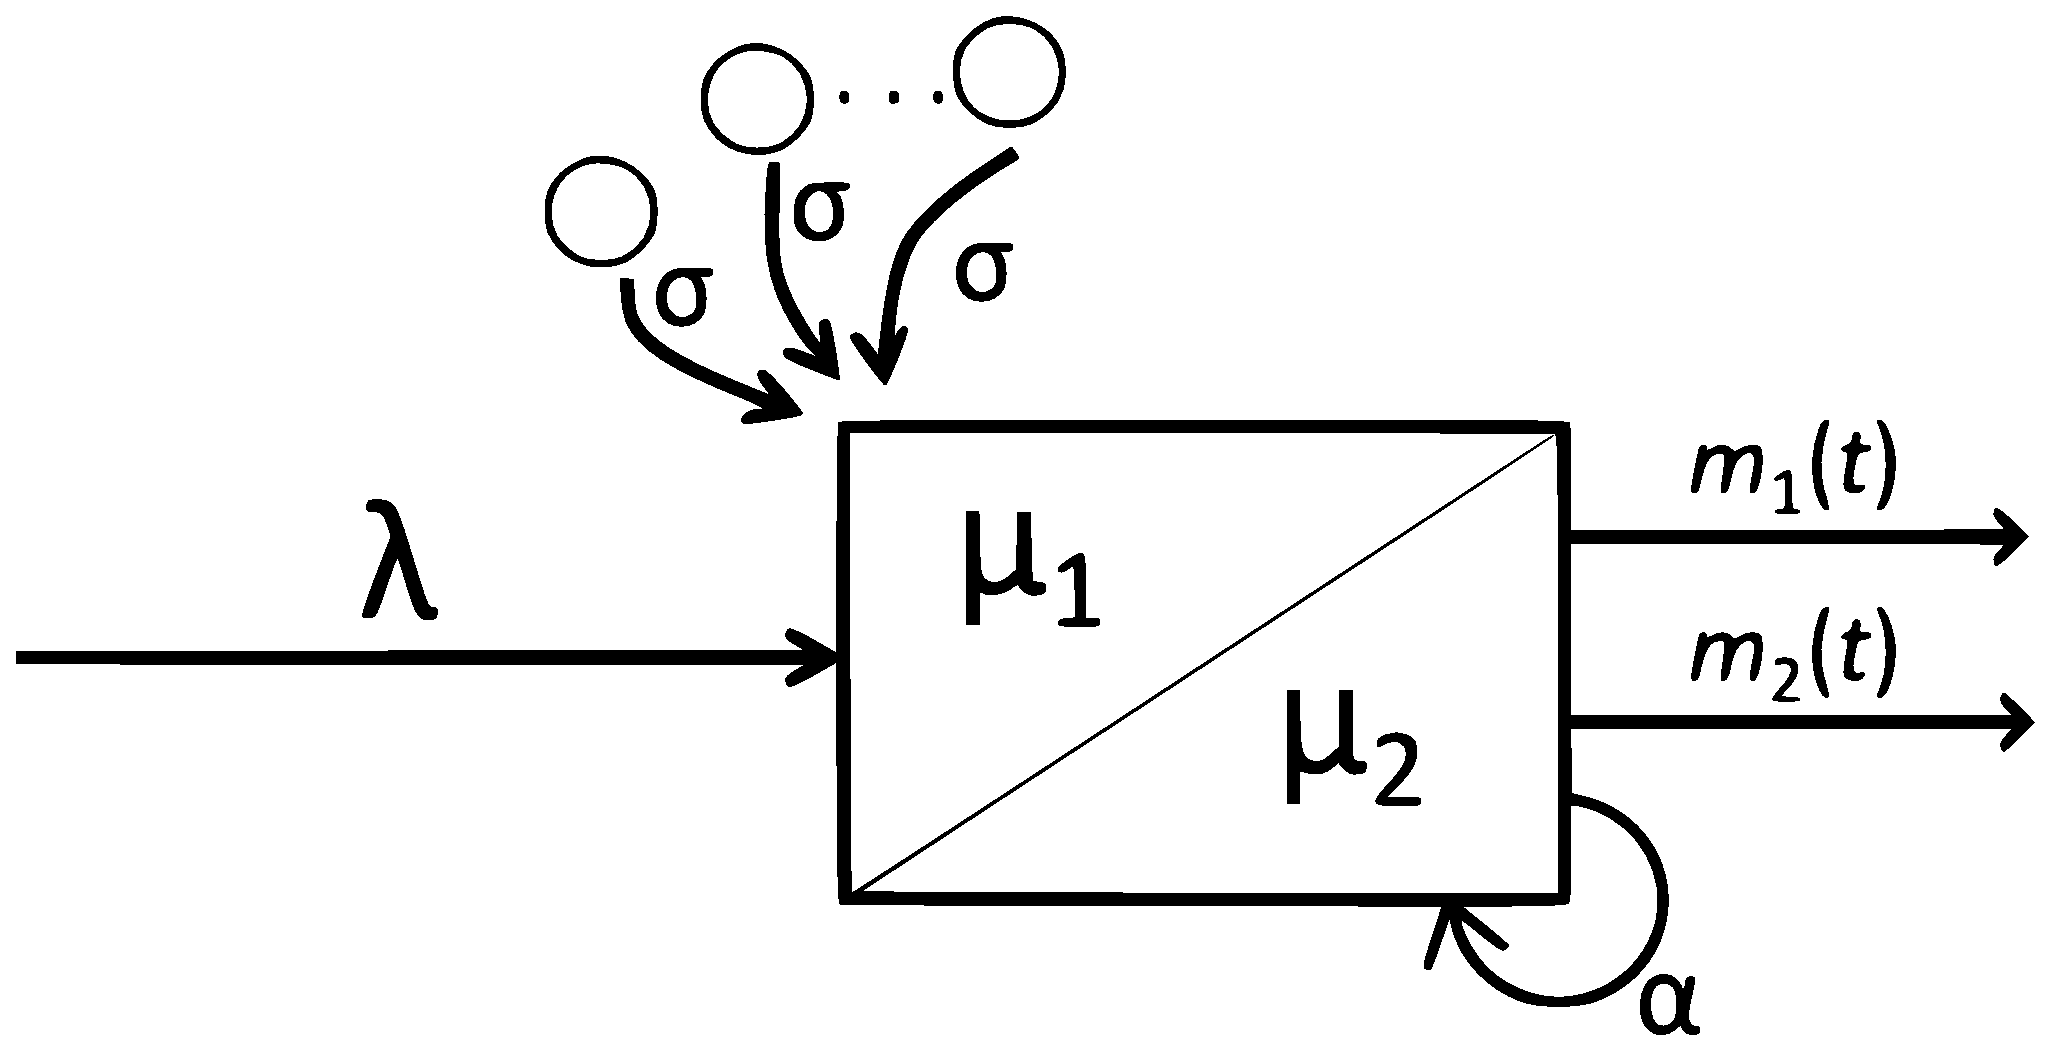
\includegraphics[scale=0.25]{twodim_output_model.eps}
	\caption{Модель RQ-системы с двумерным выходящим потоком}
	\label{twodim_output_model_fig}
\end{figure}
\subsubsection{Уравнения Колмогорова}
В данном случае, мы имеем четыре характеристики, определяющие результат функционирования системы за некоторое время $\textit{i(t)}$: состояние прибора – $\textit{k(t)}$, количество заявок на орбите – $\textit{i(t)}$, количество обслуженных заявок входящего потока – $m_{1}(t)$, количество обслуженных вызванных заявок – $m_{2}(t)$,  что можно представить в виде четырех-мерного Марковского процесса
\begin{equation*}
	\{k(t),i(t),m_{1}(t),m_{2}(t)\}
\end{equation*}
Аналогично системе с суммарным выходящим потоком, следующее состояние зависит от предыдущего, вероятность принятия прибором одного из трех состояний задается, как
\begin{equation*}
	\begin{split}
		P\{k(t)=0,i(t)=i,m_{1}(t)=m_{1},m_{2}(t)=m_{2}\} &=P_{0}(i,m_{1},m_{2},t)\\
		P\{k(t)=1,i(t)=i,m_{1}(t)=m_{1},m_{2}(t)=m_{2}\} &=P_{1}(i,m_{1},m_{2},t)\\
		P\{k(t)=2,i(t)=i,m_{1}(t)=m_{1},m_{2}(t)=m_{2}\} &=P_{2}(i,m_{1},m_{2},t)
	\end{split}
\end{equation*}
Запишем систему уравнений Колмогорова, составленную на основе введенных вероятностей перехода
\begin{equation} \label{kolmogorov_equations_twodim}
	\begin{split}
		\frac{{\partial P_{0}(i,m_{1},m_{2},t)}}{{\partial t}} &= -(\lambda + i\sigma + \alpha)P_{0}(i,m_{1},m_{2},t) + P_{1}(i,m_{1}-1,m_{2},t)\mu_{1} +\\  &+ P_{2}(i,m_{1},m_{2}-1,t)\mu_{2} ,
		\\
		\frac{{\partial P_{1}(i,m_{1},m_{2},t)}}{{\partial t}} &= -(\lambda + \mu_{1})P_{1}(i,m_{1},m_{2},t) + (i+1)\sigma P_{0}(i+1,m_{1},m_{2},t) +\\ &+ \lambda  P_{0}(i,m_{1},m_{2},t),
		\\
		\frac{{\partial P_{2}(i,m_{1},m_{2},t)}}{{\partial t}} &= -(\lambda + \mu_{2})P_{2}(i,m_{1},m_{2},t) + \lambda P_{2}(i-1,m_{1},m_{2},t)  +\\ &+ \alpha  P_{0}(i,m_{1},m_{2},t).
	\end{split}
\end{equation}	
Введем частные характеристические функции, обозначив $j=\sqrt{-1}$,
\begin{equation*}
	H_{k}(u,u_{1},u_{2},t) = \sum_{i=0}^{\infty}
	\sum_{m_{1}=0}^{\infty}
	\sum_{m_{2}=0}^{\infty}  
	e^{jui}e^{ju_{1}m_{1}}e^{ju_{2}m_{2}} P_{k}(i,m_{1},m_{2},t).
\end{equation*}
Тогда перепишем систему (\ref{kolmogorov_equations_twodim}) в виде
\begin{equation} \label{characteristic_equations_twodim}
	\begin{split}
		\frac{{\partial H_{0}(u,u_{1},u_{2},t)}}{{\partial t}} &= -(\lambda + \alpha)H_{0}(u,u_{1},u_{2},t) + j\sigma
		\frac{{\partial H_{0}(u,u_{1},u_{2},t)}}{{\partial u}} +\\  &+ \mu_{1} e^{ju_{1}}H_{1}(u,u_{1},u_{2},t) + \mu_{2}e^{ju_{2}}H_{2}(u,u_{1},u_{2},t) ,
		\\
		\frac{{\partial H_{1}(u,u_{1},u_{2},t)}}{{\partial t}} &= -(\lambda + \mu_{1})H_{1}(u,u_{1},u_{2},t) - j\sigma e^{-ju}
		\frac{{\partial H_{0}(u,u_{1},u_{2},t)}}{{\partial u}} +\\  &+ \lambda H_{0}(u,u_{1},u_{2},t) + \lambda e^{ju}H_{1}(u,u_{1},u_{2},t) ,
		\\
		\frac{{\partial H_{2}(u,u_{1},u_{2},t)}}{{\partial t}} &= -(\lambda + \mu_{2})H_{2}(u,u_{1},u_{2},t)  + \lambda e^{ju}H_{2}(u,u_{1},u_{2},t) +\\  &+ \alpha H_{0}(u,u_{1},u_{2},t).
	\end{split}
\end{equation}  
Бесконечное количество уравнений сведено к трем.

\subsubsection{Метод асимптотического анализа}
Полученную систему дифференциальных уравнений в частичных производных  (\ref{characteristic_equations_twodim}) будем решать методом асимптотического анализа в предельном условии большой задержки заявок на орбите ($\sigma \xrightarrow{} 0$).

Обозначим $\epsilon = \sigma,   u= \epsilon w,   F_{k}(w,u_{1},u_{2},t,\epsilon) = H_{k}(u,u_{1},u_{2},t)$, тогда система запишется в виде
\begin{equation} \label{asymptotic_equations_twodim}
	\begin{split}
		\frac{{\partial F_{0}(w,u_{1},u_{2},t,\epsilon)}}{{\partial t}} &= -(\lambda + \alpha)F_{0}(w,u_{1},u_{2},t,\epsilon) + j
		\frac{{\partial F_{0}(w,u_{1},u_{2},t,\epsilon)}}{{\partial w}} +\\  &+ \mu_{1} e^{ju_{1}}F_{1}(w,u_{1},u_{2},t,\epsilon) + \mu_{2}e^{ju_{2}}F_{2}(u,u_{1},u_{2},t,\epsilon) ,
		\\
		\frac{{\partial F_{1}(w,u_{1},u_{2},t,\epsilon)}}{{\partial t}} &= -(\lambda + \mu_{1})F_{1}(w,u_{1},u_{2},t,\epsilon) - j e^{-j\epsilon w}
		\frac{{\partial F_{0}(w,u_{1},u_{2},t,\epsilon)}}{{\partial w}} +\\  &+ \lambda F_{0}(w,u_{1},u_{2},t,\epsilon) + \lambda e^{j\epsilon w}F_{1}(w,u_{1},u_{2},t,\epsilon) ,
		\\
		\frac{{\partial F_{2}(w,u_{1},u_{2},t,\epsilon)}}{{\partial t}} &= -(\lambda + \mu_{2})F_{2}(w,u_{1},u_{2},t,\epsilon)  + \lambda e^{j\epsilon w}F_{2}(w,u_{1},u_{2},t,\epsilon) +\\  &+ \alpha F_{0}(w,u_{1},u_{2},t,\epsilon).
	\end{split}
\end{equation}  
Затем, что используя условие согласованности многомерных распределений, характеристическая функция процессов $m_{1}(t$) и $m_{1}(t)$ будет записана в следующем виде с введенными функциями 
\begin{equation*}
	M\{\exp(ju_{1}m_{1}(t))\exp(ju_{2}m_{2}(t))\}=\sum_{k=0}^{2}H_{k}(0,u_{1},u_{2},t) = \sum_{k=0}^{2}F_{k}(0,u_{1},u_{2},t,\epsilon).
\end{equation*}

\begin{theorem}
	Асимптотические приближение двумерной характеристической функции числа обслуженных заявок входящего потока и числа обслуженных вызванных заявок за некоторое время $t$ имеет вид
	\begin{equation*} \label{theorem_twodim}
		\begin{split}
			\boldsymbol{F}(u_{1},u_{2},t) =  \lim_{\sigma \xrightarrow{} 0} M\{\exp(ju_{1}m_{1}(t))\exp(ju_{2}m_{2}(t))\} &= 
			\\
			= \lim_{\epsilon \xrightarrow{} 0} \sum_{k=0}^{2}F_{k}(0,u_{1},u_{2},t,\epsilon) = \boldsymbol{R} \cdot \exp\{G(u_{1},u_{2})t\} \cdot \boldsymbol{E}
		\end{split}
	\end{equation*}
	где 
	\begin{equation*}
		\boldsymbol{G}(u_{1},u_{2})=\begin{bmatrix}
			-(\lambda + \alpha + \kappa) & \mu_{1}e^{ju_{1}} &  \mu_{2}e^{ju_{2}}\\
			\kappa+\lambda & -\mu_{1} & 0\\
			\alpha & 	0 &	-\mu_{2}
		\end{bmatrix}^{T},
	\end{equation*}
	вектор-строка $\boldsymbol{R}=\{R_{0},R_{1},R_{2}\}$ - стационарное распределение вероятности состояния прибора
	\begin{equation*}
		\boldsymbol{R}=\{\frac{\mu_{2}(\mu_{1} - \lambda)}{\mu_{1}(\mu_{2} - \alpha)},\frac{\lambda}{\mu_{1}},\frac{\alpha(\mu_{1} - \lambda)}{\mu_{1}(\mu_{2} + \alpha)}\},
	\end{equation*}
	$\kappa$ - нормированное среднее число заявок на орбите
	\begin{equation*}
		\kappa = \frac{\lambda(\lambda \mu_{2} + \alpha \mu_{1})}{\mu_{2}(\mu_{1} - \lambda)},
	\end{equation*}
	а $\boldsymbol{E}$ - единичный вектор-столбец соответствующей размерности.
\end{theorem}
\begin{proof}
	Делая предельный переход $ \lim_{\epsilon \xrightarrow{} 0} F_{k}(w,u_{1},u_{2},t,\epsilon) = F_{k}(w,u_{1},u_{2},t)$  в полученной системе (\ref{asymptotic_equations_twodim}) , система уравнений будет записана в виде
	\begin{equation} \label{eps_limit_twodim}
		\begin{split}
			\frac{{\partial F_{0}(w,u_{1},u_{2},t)}}{{\partial t}} &= -(\lambda + \alpha)F_{0}(w,u_{1},u_{2},t) + j
			\frac{{\partial F_{0}(w,u_{1},u_{2},t)}}{{\partial w}} +\\  &+ \mu_{1} e^{ju_{1}}F_{1}(w,u_{1},u_{2},t) + \mu_{2}e^{ju_{2}}F_{2}(w,u_{1},u_{2},t) ,
			\\
			\frac{{\partial F_{1}(w,u_{1},u_{2},t)}}{{\partial t}} &= -(\lambda + \mu_{1})F_{1}(w,u_{1},u_{2},t) - j 
			\frac{{\partial F_{0}(w,u_{1},u_{2},t)}}{{\partial w}} +\\  &+ \lambda F_{0}(w,u_{1},u_{2},t) + \lambda F_{1}(w,u_{1},u_{2},t) ,
			\\
			\frac{{\partial F_{2}(w,u_{1},u_{2},t)}}{{\partial t}} &= -(\lambda + \mu_{2})F_{2}(w,u_{1},u_{2},t)  + \lambda F_{2}(w,u_{1},u_{2},t) +\\  &+ \alpha F_{0}(w,u_{1},u_{2},t).
		\end{split}
	\end{equation}  
	Решение системы (\ref{eps_limit_twodim}) будет получено в следующей форме
	\begin{equation} \label{solution_twodim}
		F_{k}(w,u_{1},u_{2},t) = \Phi(w)F_{k}(u_{1},u_{2},t).
	\end{equation}  
	$\Phi(w)$ - асимптотическое приближение характеристической функции числа заявок на орбите при условии большой задержки на орбите.
	
	Подставив (\ref{solution_twodim}) в систему (\ref{eps_limit_twodim}) и разделив обе части уравнений на $\Phi(w)$, получим
	\begin{equation} \label{preresult_twodim}
		\begin{split}
			\frac{{\partial F_{0}(u_{1},u_{2},t)}}{{\partial t}} &= -(\lambda + \alpha)F_{0}(u_{1},u_{2},t) + j
			\frac{\Phi'(w) }{\Phi(w)}F_{0}(u_{1},u_{2},t) +\\  &+ \mu_{1} e^{ju_{1}}F_{1}(u_{1},u_{2},t) + \mu_{2}e^{ju_{2}}F_{2}(u_{1},u_{2},t) ,
			\\
			\frac{{\partial F_{1}(u_{1},u_{2},t)}}{{\partial t}} &= -(\lambda + \mu_{1})F_{1}(u_{1},u_{2},t) - j 
			\frac{\Phi'(w) }{\Phi(w)}F_{0}(u_{1},u_{2},t) +\\  &+ \lambda F_{0}(u_{1},u_{2},t) + \lambda F_{1}(u_{1},u_{2},t) ,
			\\
			\frac{{\partial F_{2}(u_{1},u_{2},t)}}{{\partial t}} &= -(\lambda + \mu_{2})F_{2}(u_{1},u_{2},t)  + \lambda F_{2}(u_{1},u_{2},t) +\\  &+ \alpha F_{0}(u_{1},u_{2},t).
		\end{split}
	\end{equation}  
	Заметим, что $w$ содержится только в отношении $\frac{\Phi'(w) }{\Phi(w)}$, а остальные слагаемые и левые части уравнений не зависят от $w$. Это означает, что  $\Phi(w)$ имеет вид экспоненты. Учитывая, что  $\Phi(w)$ имеет смысл асимптотического приближения характеристической функции числа заявок на орбите, мы можем конкретизировать вид данной функции
	\begin{equation*}
		\frac{\Phi'(w) }{\Phi(w)} = \frac{e^{j\kappa w}j\kappa}{e^{j\kappa w}},
	\end{equation*} 
	где $\kappa$ - нормированное среднее число заявок на орбите, которое было получено в \cite{nazarov2017asymptotic} и имеет вид 
	\begin{equation*}
		\kappa = \frac{\lambda(\lambda \mu_{2} + \alpha \mu_{1})}{\mu_{2}(\mu_{1} - \lambda)}.
	\end{equation*}
	
	Исходя из этого, система (\ref{preresult_twodim}) примет следующий вид
	\begin{equation} \label{result_twodim}
		\begin{split}
			\frac{{\partial F_{0}(u_{1},u_{2},t)}}{{\partial t}} &= -(\lambda + \alpha+ \kappa)F_{0}(u_{1},u_{2},t) + \\  &+ \mu_{1} e^{ju_{1}}F_{1}(u_{1},u_{2},t) + \mu_{2}e^{ju_{2}}F_{2}(u_{1},u_{2},t) ,
			\\
			\frac{{\partial F_{1}(u_{1},u_{2},t)}}{{\partial t}} &= (\lambda + \kappa)F_{0}(u_{1},u_{2},t) -  
			\mu_{1}F_{1}(u_{1},u_{2},t) +\\  &+  0F_{2}(u_{1},u_{2},t) ,
			\\
			\frac{{\partial F_{2}(u_{1},u_{2},t)}}{{\partial t}} &= \alpha F_{0}(u_{1},u_{2},t)   +  0F_{1}(u_{1},u_{2},t) -\\  &- \mu_{2}F_{2}(u_{1},u_{2},t).
		\end{split}
	\end{equation}  
	Введем следующие обозначения
	\begin{equation*}
		\boldsymbol{F}(u_{1},u_{2},t) = \{F_{0}(u_{1},u_{2},t),F_{1}(u_{1},u_{2},t),F_{1}(u_{2},u_{2},t)\},
	\end{equation*}  
	\begin{equation*}
		\boldsymbol{G}(u_{1},u_{2})=\begin{bmatrix}
			-(\lambda + \alpha + \kappa) & \mu_{1}e^{ju_{1}} &  \mu_{2}e^{ju_{2}}\\
			\kappa+\lambda & -\mu_{1} & 0\\
			\alpha & 	0 &	-\mu_{2}
		\end{bmatrix}^{T},
	\end{equation*}
	$\boldsymbol{G}(u_{1},u_{2})$ - транспонированная матрица коэффициентов системы (\ref{result_twodim}).
	Тогда получим следующее матричное уравнение
	\begin{equation*}
		\frac{{\partial \boldsymbol{F}(u_{1},u_{2},t)}}{{\partial t}} =\boldsymbol{F}(u_{1},u_{2},t)\boldsymbol{G}(u_{1},u_{2}),
	\end{equation*}
	общее решение которого имеет вид
	\begin{equation} \label{diff_twodim}
		\boldsymbol{F}(u_{1},u_{2},t)=\boldsymbol{C}e^{\boldsymbol{G}(u_{1},u_{2})t}.
	\end{equation}
	Для того, чтобы получить единственное решение, которое соответствует поведению рассматриваемой системы, примем в рассмотрение начальное условие
	\begin{equation} \label{cauchi_condition_twodim}
		\boldsymbol{F}(u_{1},u_{2},0)=\boldsymbol{R},
	\end{equation}
	где вектор-строка $\boldsymbol{R}$ - стационарное распределение вероятности состояния прибора, то есть процесса $k(t)$, которое имеет форму \cite{nazarov2017asymptotic}
	\begin{equation*}
		\boldsymbol{R}=\{\frac{\mu_{2}(\mu_{1} - \lambda)}{\mu_{1}(\mu_{2} - \alpha)},\frac{\lambda}{\mu_{1}},\frac{\alpha(\mu_{1} - \lambda)}{\mu_{1}(\mu_{2} + \alpha)}\}.
	\end{equation*}
	Описав начальное условие, мы можем перейти к решению задачи Коши (\ref{diff_twodim}, \ref{cauchi_condition_twodim}).
	
	Поскольку нас интересует распределение вероятностей количества заявок в выходных процессах, необходимо найти маргинальное распределение. Для этого суммируем компоненты вектор-строки $\boldsymbol{F}(u_{1},u_{2},t)$ по $k$ и умножаем результат на единичный вектор-столбец $\boldsymbol{E}$. Получим
	\begin{equation}\label{approximation_twodim}
		\boldsymbol{F}(u_{1},u_{2},t)\boldsymbol{E}=\boldsymbol{R}e^{\boldsymbol{G}(u_{1},u_{2})t}\boldsymbol{E}.
	\end{equation}
	Эта формула позволяет найти асимптотическое приближение характеристической функции количества вызванных и входящих заявок, обслуженных системой к некоторому моменту времени $t$. Другими словами, формула (\ref{approximation_twodim}) является решением рассматриваемой системы. 
\end{proof}

\subsubsection{Переход к явному распределению вероятности}
Полученная характеристическая функция (\ref{approximation_twodim}) так же, как и распределение вероятности, полностью описывает процессы $m_{1}(t)$ и $m_{2}(t)$, однако делает это в неявной форме. Поэтому, для использования полученной формулы для расчетов, необходимо получить из нее распределение вероятности.
Но сначала заметим, что формула (\ref{approximation_twodim}) содержит матричную экспоненту, которая не может быть вычислена в ее текущем виде. Для ее вычисления воспользуемся преобразованием подобия \cite{bronson1991matrix}, которое имеет следующий вид
\begin{equation*}
	\boldsymbol{G}(u_{1},u_{2}) =\boldsymbol{T}(u_{1},u_{2})\boldsymbol{GJ}(u_{1},u_{2})\boldsymbol{T}(u_{1},u_{2})^{-1},
\end{equation*}
где $\boldsymbol{T}(u_{1},u_{2})$ – матрицы собственных вектором матрицы $\boldsymbol{G}(u_{1},u_{2})$, а $\boldsymbol{GJ}(u_{1},u_{2})$ - диагональная матрицы, содержащая собственные числа $\boldsymbol{G}(u_{1},u_{2})$. Данное преобразование справедливо для любой степени $m$ некоторой матрицы $\boldsymbol{A}^{m}$, из чего следует, что оно так же справедливо для матричной экспоненты \ref{egorov2006prog}
\begin{equation*}
	e^{\boldsymbol{G}(u_{1},u_{2})t}=\boldsymbol{T}(u_{1},u_{2})\cdot \begin{bmatrix}
		e^{t \Lambda_{1}(u_{1},u_{2})} & 0 &  0\\
		0 & e^{t \Lambda_{2}(u_{1},u_{2})} & 0\\
		0 & 0 &	e^{t \Lambda_{3}(u_{1},u_{2})}
	\end{bmatrix} \cdot \boldsymbol{T}(u_{1},u_{2})^{-1},
\end{equation*}
где $\Lambda_{n}$ - собственное число матрицы $\boldsymbol{G}(u_{1},u_{2})$. Тогда распределение примет следующий вид
\begin{equation*}
	\boldsymbol{F}(u_{1},u_{2},t)=\boldsymbol{R} \cdot \boldsymbol{T}(u_{1},u_{2})\cdot \begin{bmatrix}
		e^{t \Lambda_{1}(u_{1},u_{2})} & 0 &  0\\
		0 & e^{t \Lambda_{2}(u_{1},u_{2})} & 0\\
		0 & 0 &	e^{t \Lambda_{3}(u_{1},u_{2})}
	\end{bmatrix} \cdot \boldsymbol{T}(u_{1},u_{2})^{-1} \cdot \boldsymbol{E}.
\end{equation*}
Для получения распределения воспользуемся свойством характеристической функции, из которого следует, что распределение всегда восстанавливается из характеристической функции. Для восстановления будем использовать обратное преобразование Фурье для дискретных величин
\begin{equation*}
	P(m_{1},m_{2},t) = \dfrac{1}{2\pi}\int_{-\pi}^{\pi}\int_{-\pi}^{\pi} e^{-i \cdot u_{1} \cdot m_{1}} e^{-i \cdot u_{2} \cdot m_{2}}\boldsymbol{F}(u_{1},u_{2},t)du_{2}du_{2}.
\end{equation*}
Полученная формула характеризует вероятность обслуживания $m_{1}$ входящих заявок и $m_{2}$ вызванных заявок к моменту времени $t$ в рассматриваемой системе.

\subsubsection{Коэффициент корреляции}
Полученное асимптотические приближение характеристической функции (\ref{approximation_twodim}) позволяет нам подробнее изучить выходящие потоки рассматриваемой системы, а именно – найти корреляционную зависимость случайных процессов $m_{1}(t)$ и $m_{2}(t)$.
Рассмотрим нахождение коэффициента корреляции, который будет зависеть от параметра $t$
\begin{equation*}
	r(t) = \frac{\textnormal{cov}(m_{1}(t),m_{2}(t))}{\sqrt{D(m_{1}(t))}\sqrt{D(m_{2}(t))}}.
\end{equation*}
Воспользуемся свойством характеристической функции о существовании ее $n$-ой производной, соответствующей $n$-му начальному моменту случайной величины. Тогда ковариация и дисперсия будут вычисляться следующим образом
\begin{equation*}
	\begin{split}
		\textnormal{cov}(m_{1}(t),m_{2}(t)) &= M\{m_{1}(t)m_{2}(t)\} - M\{m_{1}(t)\}M\{m_{2}(t)\} = \frac{1}{j^{2}}\frac{{\partial}^{2}}{{\partial u_{1}}{\partial u_{2}}}\boldsymbol{F}(u_{1},u_{2},t) \bigg\rvert_{\substack{u_{1} = 0 \\ u_{2} = 0}} - \\ &- \frac{1}{j^{2}} \frac{{\partial}}{{\partial u_{1}}} \boldsymbol{F}(u_{1},u_{2},t) \bigg\rvert_{\substack{u_{1} = 0 \\ u_{2} = 0}} \frac{{\partial}}{{\partial u_{2}}} \boldsymbol{F}(u_{1},u_{2},t) \bigg\rvert_{\substack{u_{1} = 0 \\ u_{2} = 0}},
		\\
		D\{m_{1}(t)\} &= M^{2}\{m_{1}(t)\} - (M\{m_{1}(t)\})^{2} = \frac{1}{j^{2}}\frac{{\partial}^{2}}{{\partial u_{1}}^{2}}\boldsymbol{F}(u_{1},u_{2},t) \bigg\rvert_{\substack{u_{1} = 0 \\ u_{2} = 0}}  - \\ &- (\frac{1}{j^{2}} \frac{{\partial}}{{\partial u_{1}}} \boldsymbol{F}(u_{1},u_{2},t) \bigg\rvert_{\substack{u_{1} = 0 \\ u_{2} = 0}})^{2},
		\\
		D\{m_{2}(t)\} &= M^{2}\{m_{2}(t)\} - (M\{m_{2}(t)\})^{2} = \frac{1}{j^{2}}\frac{{\partial}^{2}}{{\partial u_{2}}^{2}}\boldsymbol{F}(u_{1},u_{2},t) \bigg\rvert_{\substack{u_{1} = 0 \\ u_{2} = 0}}  - \\ &- (\frac{1}{j^{2}} \frac{{\partial}}{{\partial u_{2}}} \boldsymbol{F}(u_{1},u_{2},t) \bigg\rvert_{\substack{u_{1} = 0 \\ u_{2} = 0}})^{2}.
	\end{split}
\end{equation*}
Полученные формулы позволяют использовать нам численно исследовать поведение системы при разных параметрах.
\clearpage
 %Простейший поток
\section {Исследование систем с MMPP-потоком}
В этом разделе предлагается к рассмотрению система обслуживания, в которой в качестве источника входящих заявок выступает MMPP-поток.

MMPP (Markov Modulated Poisson Process) представляет собой поток заявок, управляемый непрерывной цепью Маркова. Изменение состояния влекёт за собой изменение интенсивности прихода заявок. Данный тип входящего потока широко используется для моделирования телекомуникационных сетей, поскольку он точно описывает изменяющуюся во времени скорость поступления заявок и фиксирует некоторые важные корреляции между временами прибытия, оставаясь при этом поддающимся анализу \cite{fischer1993markov}.
 


Для того, чтобы описать изменение состояние MMPP-потока во времени используются две матрицы.

Матрица инфинитезимальных характеристик $Q$. Величина $q_{ij}$ определяет интенсивность перехода процесса из $i$-ого в $j$-ое состояние, а величина $-q_{ii}$ - интенсивность выхода из состояния $i$.
Матрица $Q$ имеет свойство - $\sum_{j}q_{ij} = 0$
\begin{equation*}
	\boldsymbol{Q}=\begin{bmatrix}
		q_{11} &  \dots &  q_{1n}\\
		\vdots & \ddots &  \\
		q_{n1} &    	&	q_{nn}
	\end{bmatrix}
\end{equation*}
Диагональная матрица $\Lambda$ задаёт интенсивность поступления заявок для каждого из состояний процесса.
\begin{equation*}
	\boldsymbol{\Lambda}=\begin{bmatrix}
		\lambda_{11}&	\dots	&   	 & 0\\
		\vdots 		&\lambda_{22}&  	 &   \\
		       		&    		& \ddots &   \\
		0  			&   \dots 	&		 & \lambda_{nn}
	\end{bmatrix}
\end{equation*}

\subsection{RQ--система с входящим MMPP и двумерным выходящим потоком} \label{section_map_twodim}
В случае RQ--системы с MMPP--потоком, к описанной ранее общей модели добавляется так же процесс $n_(t)$ --- состояние входящего потока в момент времени $t$. Тогда, результат функционирования системы будет описываться пяти--мерным Марковским процессом
\begin{equation*}
	\{k(t),n(t),i(t),m_{1}(t),m_{2}(t)\}.
\end{equation*}

\subsubsection{Уравнения Колмогорова}
Исходя из описанного Марковского процесса, вероятности того, что прибор будет находится в одном из трех состояний $k$, на орбите будет $i$ заявок, $m_{1}$ заявок входящего потока и $m_{2}$ вызванных заявок будет обслужено, а управляющая MMPP--потоком цепь Маркова будет находится в состоянии $n$, будут иметь вид
\begin{equation*}
	\begin{split}
		P\{k(t)=0,n(t)=n,i(t)=i,m_{1}(t)=m_{1},m_{2}(t)=m_{2}\} &=P_{0}(n,i,m_{1},m_{2},t),\\
		P\{k(t)=1,n(t)=n,i(t)=i,m_{1}(t)=m_{1},m_{2}(t)=m_{2}\} &=P_{1}(n,i,m_{1},m_{2},t),\\
		P\{k(t)=2,n(t)=n,i(t)=i,m_{1}(t)=m_{1},m_{2}(t)=m_{2}\} &=P_{2}(n,i,m_{1},m_{2},t).
	\end{split}
\end{equation*} 

На основе данных вероятностей запишем систему уравнений Колмогорова с учетом текущего состояния входящего потока
\begin{equation} \label{kolmogorov_equations_twodim_map}
	\begin{split}
		\frac{{\partial P_{0}(n,i,m_{1},m_{2},t)}}{{\partial t}} &= -(\lambda_{n} + i\sigma + \alpha)P_{0}(n,i,m_{1},m_{2},t) + P_{1}(n,i,m_{1}-1,m_{2},t)\mu_{1} +\\  &+ P_{2}(n,i,m_{1},m_{2}-1,t)\mu_{2} + \sum_{v=1}^{N} P_{0}(v,i,m_{1},m_{2},t)q_{vn},
		\\
		\frac{{\partial P_{1}(n,i,m_{1},m_{2},t)}}{{\partial t}} &= -(\lambda_{n} + \mu_{1})P_{1}(n,i,m_{1},m_{2},t) + (i+1)\sigma P_{0}(n,i+1,m_{1},m_{2},t) +\\ &+ \lambda_{n}  P_{0}(i,m_{1},m_{2},t) + \sum_{v=1}^{N}P_{1}(v,i,m_{1},m_{2},t)q_{vn},
		\\
		\frac{{\partial P_{2}(n,i,m_{1},m_{2},t)}}{{\partial t}} &= -(\lambda_{n} + \mu_{2})P_{2}(n,i,m_{1},m_{2},t) + \lambda_{n} P_{2}(n,i-1,m_{1},m_{2},t)  +\\ &+ \alpha  P_{0}(n,i,m_{1},m_{2},t) +  \sum_{v=1}^{N}P_{2}(v,i,m_{1},m_{2},t)q_{vn}.
	\end{split}
\end{equation}	

Введем частные характеристические функции, обозначив $j=\sqrt{-1}$
\begin{equation*}
	H_{k}(n,u,u_{1},u_{2},t) = \sum_{i=0}^{\infty}
	\sum_{m_{1}=0}^{\infty}
	\sum_{m_{2}=0}^{\infty}  
	e^{jui}e^{ju_{1}m_{1}}e^{ju_{2}m_{2}} P_{k}(n,i,m_{1},m_{2},t).
\end{equation*}
Перепишем систему \eqref{kolmogorov_equations_twodim_map} с учетом введенных частных характеристических функций
\begin{equation} \label{characteristic_equations_twodim_map}
	\begin{split}
		\frac{{\partial H_{0}(n,u,u_{1},u_{2},t)}}{{\partial t}} &= -(\lambda_{n} + \alpha)H_{0}(n,u,u_{1},u_{2},t) + j\sigma
		\frac{{\partial H_{0}(n,u,u_{1},u_{2},t)}}{{\partial u}} +\\  &+ \mu_{1} e^{ju_{1}}H_{1}(n,u,u_{1},u_{2},t) + \mu_{2}e^{ju_{2}}H_{2}(n,u,u_{1},u_{2},t) +\\  &+ \sum_{v=1}^{N}H_{0}(v,u,u_{1},u_{2},t)q_{vn} ,
		\\
		\frac{{\partial H_{1}(n,u,u_{1},u_{2},t)}}{{\partial t}} &= -(\lambda_{n} + \mu_{1})H_{1}(n,u,u_{1},u_{2},t) - j\sigma e^{-ju}
		\frac{{\partial H_{0}(n,u,u_{1},u_{2},t)}}{{\partial u}} +\\  &+ \lambda_{n} H_{0}(n,u,u_{1},u_{2},t) + \lambda_{n} e^{ju}H_{1}(n,u,u_{1},u_{2},t) +\\  &+ \sum_{v=1}^{N}H_{1}(v,u,u_{1},u_{2},t)q_{vn} ,
		\\
		\frac{{\partial H_{2}(n,u,u_{1},u_{2},t)}}{{\partial t}} &= -(\lambda_{n} + \mu_{2})H_{2}(n,u,u_{1},u_{2},t)  + \lambda_{n} e^{ju}H_{2}(n,u,u_{1},u_{2},t) +\\  &+ \alpha H_{0}(n,u,u_{1},u_{2},t) + \sum_{v=1}^{N}H_{2}(v,u,u_{1},u_{2},t)q_{vn}.
	\end{split}
\end{equation}  

Для дальнейшего анализа введем следующие обозначения
\begin{equation*}	
\boldsymbol{H}_{k}(u,u_{1},u_{2},t) = \{H_{k}(1,u,u_{1},u_{2},t),H_{k}(2,u,u_{1},u_{2},t),\dots,H_{k}(N,u,u_{1},u_{2},t)\},
\end{equation*}
а так же диагональную единичную матрицу $\boldsymbol{I}$ размера $N$.
Тогда система \eqref{characteristic_equations_twodim_map} примет вид
\begin{equation} \label{characteristic_equations_twodim_map_matrix}
	\begin{split}
		\frac{{\partial \boldsymbol{H}_{0}(u,u_{1},u_{2},t)}}{{\partial t}} &= (\boldsymbol{Q}-\boldsymbol{\Lambda}-\alpha\boldsymbol{I})\boldsymbol{H}_{0}(u,u_{1},u_{2},t) + \mu_{1} e^{ju_{1}}\boldsymbol{H}_{1}(n,u,u_{1},u_{2},t)  + \\  &+ \mu_{2}e^{ju_{2}}\boldsymbol{H}_{2}(u,u_{1},u_{2},t) + j\sigma
		\frac{{\partial \boldsymbol{H}_{0}(u,u_{1},u_{2},t)}}{{\partial u}},
		\\
		\frac{{\partial \boldsymbol{H}_{1}(u,u_{1},u_{2},t)}}{{\partial t}} &= \boldsymbol{\Lambda} \boldsymbol{H}_{0}(u,u_{1},u_{2},t) +  (\boldsymbol{Q}+(e^{ju}-1)\boldsymbol{\Lambda} - \boldsymbol{I}\mu_{1})\boldsymbol{H}_{1}(u,u_{1},u_{2},t) -\\ &- j\sigma e^{-ju}
		\frac{{\partial \boldsymbol{H}_{0}(u,u_{1},u_{2},t)}}{{\partial u}},
		\\
		\frac{{\partial \boldsymbol{H}_{2}(u,u_{1},u_{2},t)}}{{\partial t}} &= \alpha \boldsymbol{H}_{0}(u,u_{1},u_{2},t) + (\boldsymbol{Q}+(e^{ju}-1)\boldsymbol{\Lambda} - \boldsymbol{I}\mu_{2})\boldsymbol{H}_{2}(u,u_{1},u_{2},t).
	\end{split}
\end{equation} 
\subsubsection{Метод асимптотического анализа}
Полученную систему дифференциальных уравнений \eqref{characteristic_equations_twodim_map_matrix} будем решать методом асимптотического анализа в предельном условии большой задержки заявок на орбите ($\sigma \xrightarrow{} 0$).

Обозначим $\epsilon = \sigma,   u= \epsilon w,   \boldsymbol{F}_{k}(w,u_{1},u_{2},t,\epsilon) = \boldsymbol{H}_{k}(u,u_{1},u_{2},t)$, тогда система запишется в виде
\begin{equation} \label{asymptotic_equations_twodim_map}
	\begin{split}
		\frac{{\partial \boldsymbol{F}_{0}(w,u_{1},u_{2},t,\epsilon)}}{{\partial t}} &= (\boldsymbol{Q}-\boldsymbol{\Lambda}-\alpha\boldsymbol{I})\boldsymbol{F}_{0}(w,u_{1},u_{2},t,\epsilon) + \mu_{1} e^{ju_{1}}\boldsymbol{F}_{1}(w,u_{1},u_{2},t,\epsilon)  + \\  &+ \mu_{2}e^{ju_{2}}\boldsymbol{F}_{2}(w,u_{1},u_{2},t,\epsilon) + j
	\frac{{\partial \boldsymbol{F}_{0}(w,u_{1},u_{2},t,\epsilon)}}{{\partial w}},
	\\
	\frac{{\partial \boldsymbol{F}_{1}(w,u_{1},u_{2},t,\epsilon)}}{{\partial t}} &= \boldsymbol{\Lambda} \boldsymbol{F}_{0}(w,u_{1},u_{2},t,\epsilon) +  (\boldsymbol{Q}+(e^{j\epsilon w}-1)\boldsymbol{\Lambda} - \boldsymbol{I}\mu_{1})\cdot \\ &\cdot \boldsymbol{F}_{1}(w,u_{1},u_{2},t,\epsilon) - j e^{-j\epsilon w}
	\frac{{\partial \boldsymbol{F}_{0}(w,u_{1},u_{2},t,\epsilon)}}{{\partial w}},
	\\
	\frac{{\partial \boldsymbol{F}_{2}(w,u_{1},u_{2},t,\epsilon)}}{{\partial t}} &= \alpha \boldsymbol{F}_{0}(w,u_{1},u_{2},t,\epsilon) + (\boldsymbol{Q}+(e^{j\epsilon w}-1)\boldsymbol{\Lambda} - \boldsymbol{I}\mu_{2})\boldsymbol{F}_{2}(w,u_{1},u_{2},t,\epsilon).
	\end{split}
\end{equation}  

Решение системы \eqref{asymptotic_equations_twodim_map} будет сформулировано в последующих теоремах.

\begin{theorem} \label{R_theorem}
	Пусть $i(t)$ --- количество заявок на орбите в системе с входящим MMPP--потоком и вызываемыми заявками, тогда в стационарном режиме мы получим
	\begin{equation*}
		\lim_{\epsilon \xrightarrow{} 0}\{\sum_{k=0}^{2}F_{k}(w,0,0,t,\epsilon)\} = \lim_{\sigma \xrightarrow{} 0} M e^{jw\sigma i(t)} = e^{jw\kappa},
	\end{equation*}
где $\kappa$ --- положительный корень уравнения
\begin{equation*}
	\kappa \boldsymbol{R}_{0}(\kappa)\boldsymbol{e} = [\boldsymbol{R}_{1}(\kappa) + \boldsymbol{R}_{2}(\kappa)]\boldsymbol{\Lambda}\boldsymbol{e}.
\end{equation*}
Более того, векторы $\boldsymbol{R}_{k}$ определяются следующим образом
\begin{equation*}
	\left\{
	\begin{aligned}
		\boldsymbol{R}_{0}(\kappa) & = \boldsymbol{r}\{\boldsymbol{I} + [\boldsymbol{\Lambda} + \kappa\boldsymbol{I}](\mu_{1}\boldsymbol{I}-\boldsymbol{Q})^{-1}+\alpha(\mu_{2}\boldsymbol{I}-\boldsymbol{Q})^{-1}\}^{-1},\\
		\boldsymbol{R}_{1}(\kappa) & = \boldsymbol{R}_{0}(\kappa)[\boldsymbol{\Lambda} + \kappa\boldsymbol{I}](\mu_{1}\boldsymbol{I} - \boldsymbol{Q})^{-1},\\
		\boldsymbol{R}_{2}(\kappa) & = \alpha\boldsymbol{R}_{0}(\kappa)(\mu_{2}\boldsymbol{I} - \boldsymbol{Q})^{-1}.
	\end{aligned}
\right.
\end{equation*}
Вектор--строка $\boldsymbol{r}$ --- стационарное распределение вероятности процесса управляющей цепи MMPP--потока $n(t)$, которое задается как единственное решение системы $\boldsymbol{r}\boldsymbol{Q} =0, \boldsymbol{r}\boldsymbol{e} = 1$.
\end{theorem}
\begin{proof}
	В системе уравнений \eqref{asymptotic_equations_twodim_map} мы обозначили $u_{1} = u_{2} = 0$, тем самым убирая процессы $m_{1}(t)$ и $m_{2}(t)$ из рассмотрения. Тогда, мы можем получить систему уравнений уже для трехмерного процесса $\{n(t),k(t),i(t)\}$, рассматривая его в стационарном режиме, что позволяет нам избавиться от производных по времени $t$.
	
	Обозначим 
	\begin{equation*}
		\boldsymbol{F}_{k}(w,\epsilon) = \lim_{t \xrightarrow{} \infty} \boldsymbol{F}_{k}(w,0,0,t,\epsilon).
	\end{equation*}
Получим следующую систему
\begin{equation}
		 \label{asymptotic_equations_twodim_map_no_time}
		 \begin{split}
		 &(\boldsymbol{Q}-\boldsymbol{\Lambda}-\alpha\boldsymbol{I})\boldsymbol{F}_{0}(w,\epsilon) + \mu_{1} \boldsymbol{F}_{1}(w,\epsilon)  +  \mu_{2}\boldsymbol{F}_{2}(w,\epsilon) + j
		 \boldsymbol{F}_{0}'(w,\epsilon)  = 0,
		\\
		 &\boldsymbol{\Lambda} \boldsymbol{F}_{0}(w,\epsilon) +  (\boldsymbol{Q}+(e^{j\epsilon w}-1)\boldsymbol{\Lambda} - \boldsymbol{I}\mu_{1})\boldsymbol{F}_{1}(w,\epsilon) - j e^{-j\epsilon w}
		 \boldsymbol{F}_{0}'(w,\epsilon)  = 0,
		\\
		&\alpha \boldsymbol{F}_{0}(w,\epsilon) + (\boldsymbol{Q}+(e^{j\epsilon w}-1)\boldsymbol{\Lambda} - \boldsymbol{I}\mu_{2})\boldsymbol{F}_{2}(w,\epsilon)  = 0.
	\end{split}
\end{equation}  
Делая в системе \eqref{asymptotic_equations_twodim_map_no_time} предельный переход $\epsilon \xrightarrow{} 0$, получим
\begin{equation}
	\label{asymptotic_equations_twodim_map_no_limit}
	\begin{split}
		&(\boldsymbol{Q}-\boldsymbol{\Lambda}-\alpha\boldsymbol{I})\boldsymbol{F}_{0}(w) + \mu_{1} \boldsymbol{F}_{1}(w)  +  \mu_{2}\boldsymbol{F}_{2}(w) + j
		\boldsymbol{F}_{0}'(w)  = 0,
		\\
		&\boldsymbol{\Lambda} \boldsymbol{F}_{0}(w) +  (\boldsymbol{Q} - \boldsymbol{I}\mu_{1})\boldsymbol{F}_{1}(w) - j
		\boldsymbol{F}_{0}'(w)  = 0,
		\\
		&\alpha \boldsymbol{F}_{0}(w) + (\boldsymbol{Q} - \boldsymbol{I}\mu_{2})\boldsymbol{F}_{2}(w)  = 0.
	\end{split}
\end{equation}

Решение данной системы будет найдено в следующей форме
\begin{equation} \label{R_solution}
	\boldsymbol{F}_{k} = \Phi(w)\boldsymbol{R}_{k},
\end{equation}
где $\boldsymbol{R}_{n}$ --- стационарное распределение вероятности прибора, а $\Phi(w)$ --- асимптотическое приближение характеристической функции числа заявок на орбите при условии большой задержки на орбите. Подставляя \eqref{R_solution} в \eqref{asymptotic_equations_twodim_map_no_limit} и деля на $\Phi(w)$, получим
\begin{equation}
	\label{asymptotic_equations_twodim_map_R}
	\begin{split}
		&(\boldsymbol{Q}-\boldsymbol{\Lambda}-\alpha\boldsymbol{I})\boldsymbol{R}_{0} + \mu_{1} \boldsymbol{R}_{1}  +  \mu_{2}\boldsymbol{R}_{2} + j
		\frac{\Phi'(w) }{\Phi(w)}\boldsymbol{R}_{0}  = 0,
		\\
		&\boldsymbol{\Lambda} \boldsymbol{R}_{0} +  (\boldsymbol{Q} - \boldsymbol{I}\mu_{1})\boldsymbol{R}_{1} - j\frac{\Phi'(w) }{\Phi(w)}
		\boldsymbol{R}_{0}  = 0,
		\\
		&\alpha \boldsymbol{R}_{0} + (\boldsymbol{Q} - \boldsymbol{I}\mu_{2})\boldsymbol{R}_{2}  = 0.
	\end{split}
\end{equation}
Вид функции $\Phi(w)$ уже ранее был нами конкретизирован в \eqref{Phi_concrete} так, что $j\frac{\Phi(w)'}{\Phi(w)} = -\kappa$. 
Подставим данное выражение в систему \eqref{asymptotic_equations_twodim_map_R}, получим
\begin{equation}
	\label{asymptotic_equations_twodim_map_R_final}
	\begin{split}
		&(\boldsymbol{Q}-\boldsymbol{\Lambda}-\alpha\boldsymbol{I})\boldsymbol{R}_{0} + \mu_{1} \boldsymbol{R}_{1}  +  \mu_{2}\boldsymbol{R}_{2} -\kappa{R}_{0}  = 0,
		\\
		&\boldsymbol{\Lambda} \boldsymbol{R}_{0} +  (\boldsymbol{Q} - \boldsymbol{I}\mu_{1})\boldsymbol{R}_{1} + \kappa
		\boldsymbol{R}_{0}  = 0,
		\\
		&\alpha \boldsymbol{R}_{0} + (\boldsymbol{Q} - \boldsymbol{I}\mu_{2})\boldsymbol{R}_{2}  = 0.
	\end{split}
\end{equation}
Запишем условия нормировки для стационарного распределения вероятностей числа обслуженных заявок прибором
\begin{equation*}
	\boldsymbol{R}_{0} + \boldsymbol{R}_{1} + \boldsymbol{R}_{2} = \boldsymbol{r}.
\end{equation*}
Основываясь на этом уравнении, а также на двух последних уравнения системы \eqref{asymptotic_equations_twodim_map_R_final} запишем систему
\begin{equation} \label{R_system}
	\left\{
	\begin{aligned}
		\boldsymbol{R}_{1}& = \boldsymbol{R}_{0}[\boldsymbol{\Lambda} + \kappa\boldsymbol{I}](\mu_{1}\boldsymbol{I} - \boldsymbol{Q})^{-1},\\
		\boldsymbol{R}_{2}& = \alpha\boldsymbol{R}_{0}(\mu_2\boldsymbol{I} - \boldsymbol{Q})^{-1},\\
		\boldsymbol{R}_{0}& + \boldsymbol{R}_{1} + \boldsymbol{R}_{2} = \boldsymbol{r}.
	\end{aligned}
	\right.
\end{equation}
Просуммируем уравнения системы \eqref{asymptotic_equations_twodim_map_no_time}
\begin{equation*}
	\begin{split}
		[\boldsymbol{F}_{0}(w,\epsilon) + \boldsymbol{F}_{1}(w,\epsilon) +  \boldsymbol{F}_{2}(w,\epsilon)]\boldsymbol{Q} &+\\  + 
		\boldsymbol{F}_{1}(w,\epsilon)(e^{jw\epsilon} - 1)\boldsymbol{\Lambda} + & \boldsymbol{F}_{2}(w,\epsilon)(e^{jw\epsilon} - 1)\boldsymbol{\Lambda} + je^{-jw\epsilon}(e^{jw\epsilon} - 1)\boldsymbol{F}_{0}'(w,\epsilon) = 0.
	\end{split}
\end{equation*}
Умножая получившееся уравнения на единичный вектор столбец $\boldsymbol{e}$, получим
\begin{equation*}
	\{\boldsymbol{F}_{1}(w,\epsilon) + \boldsymbol{F}_{2}(w,\epsilon)\}\boldsymbol{\Lambda}\boldsymbol{e} + je^{-jw\epsilon}\boldsymbol{F}_{0}'(w,\epsilon)\boldsymbol{e} = 0.
\end{equation*}
Затем, подставим произведение \eqref{R_solution} в получившееся уравнение
\begin{equation*}
	[\boldsymbol{R}_{1} + \boldsymbol{R}_{2}]\boldsymbol{\Lambda}\boldsymbol{e} + j\frac{\Phi'(w)}{\Phi(w)}\boldsymbol{R}_{0}\boldsymbol{e} = 0
\end{equation*}
 и делаем замену
 \begin{equation} \label{R_kappa_exression}
 	[\boldsymbol{R}_{1} + \boldsymbol{R}_{2}]\boldsymbol{\Lambda}\boldsymbol{e} -\kappa\boldsymbol{R}_{0}\boldsymbol{e} = 0.
\end{equation}

Из \eqref{R_kappa_exression} мы можем выразить $\kappa$ с помощью $\boldsymbol{R}_{0}$,$\boldsymbol{R}_{1}$ и $\boldsymbol{R}_{2}$. Помимо этого, мы можем переписать систему \eqref{R_system} в следующим виде
\begin{equation*}
	\left\{
	\begin{aligned}
		\boldsymbol{R}_{0}(\kappa) & = \boldsymbol{r}\{\boldsymbol{I} + [\boldsymbol{\Lambda} + \kappa\boldsymbol{I}](\mu_{1}\boldsymbol{I}-\boldsymbol{Q})^{-1}+\alpha(\mu_{2}\boldsymbol{I}-\boldsymbol{Q})^{-1}\}^{-1},\\
		\boldsymbol{R}_{1}(\kappa) & = \boldsymbol{R}_{0}(\kappa)[\boldsymbol{\Lambda} + \kappa\boldsymbol{I}](\mu_{1}\boldsymbol{I} - \boldsymbol{Q})^{-1},\\
		\boldsymbol{R}_{2}(\kappa) & = \alpha\boldsymbol{R}_{0}(\kappa)(\mu_{2}\boldsymbol{I} - \boldsymbol{Q})^{-1}
	\end{aligned}
	\right.
\end{equation*}
\end{proof}
Теорема \ref{R_theorem} является вспомогательной, так как основное решение рассматриваемой системы изложено в теореме \ref{mmpp_theorem} и нуждается в полученных на данном этапе результатах, а именно --- среднее число заявок на орбите при условии их большой задержки $\kappa$ и стационарное распределение вероятностей состояния прибора $\boldsymbol{R}_{k}$.

\begin{theorem} \label{mmpp_theorem}
	Асимптотические приближение двумерной характеристической функции числа обслуженных заявок входящего MMPP-потока и числа обслуженных вызванных заявок за некоторое время $t$ имеет вид
	\begin{equation*} \label{theorem_twodim_map}
		\begin{split}
		  \lim_{\sigma \xrightarrow{} 0} M\{\exp(ju_{1}m_{1}(t))\exp(ju_{2}m_{2}(t))\} &=
			 \lim_{\epsilon \xrightarrow{} 0} \left\{ \sum_{k=0}^{2}F_{k}(0,u_{1},u_{2},t,\epsilon) \right\}\boldsymbol{e} =\\ = \boldsymbol{R} \cdot \exp\{G(u_{1},u_{2})t\}\boldsymbol{ee},
		\end{split}
	\end{equation*}
	где матрица $\boldsymbol{G}(u_{1},u_{2})$ представима в виде
	\begin{equation*}
		\boldsymbol{G}(u_{1},u_{2})=\begin{bmatrix}
			\boldsymbol{Q}-\boldsymbol{\Lambda}-(\alpha + \kappa)\boldsymbol{I} & \mu_{1}e^{ju_{1}}\boldsymbol{I} &  \mu_{2}e^{ju_{2}}\boldsymbol{I}\\
			\boldsymbol{\Lambda}+\kappa\boldsymbol{I} & \boldsymbol{Q}-\mu_{1}\boldsymbol{I} & 0\\
			\alpha\boldsymbol{I} & 	0 &	\boldsymbol{Q}-\mu_{2}\boldsymbol{I}
		\end{bmatrix}^{T},
	\end{equation*}
	вектор--строка $\boldsymbol{R}=\{\boldsymbol{R}_{0},\boldsymbol{R}_{1},\boldsymbol{R}_{2}\}$ -- двумерное стационарное распределение вероятности случайного процесса $\{k(t),n(t)\}$, где, соответственно,  $\boldsymbol{R}_{k}$ имеет размерность $N$, $\kappa$ --- нормированное среднее число заявок на орбите, а $e$ и $ee$ --- единичные вектор--столбцы размерности $N$ и $N \cdot K$ соответственно.
\end{theorem}
\begin{proof}
	Делая предельный переход $ \lim_{\epsilon \xrightarrow{} 0}\boldsymbol{F}_{k}(w,u_{1},u_{2},t,\epsilon) = \boldsymbol{F}_{k}(w,u_{1},u_{2},t)$  в полученной системе \eqref{asymptotic_equations_twodim_map}, система уравнений будет записана в виде
	\begin{equation} \label{eps_limit_twodim_map}
		\begin{split}
			\frac{{\partial \boldsymbol{F}_{0}(w,u_{1},u_{2},t)}}{{\partial t}} &= (\boldsymbol{Q}-\boldsymbol{\Lambda}-\alpha\boldsymbol{I})\boldsymbol{F}_{0}(w,u_{1},u_{2},t) + \mu_{1} e^{ju_{1}}\boldsymbol{F}_{1}(w,u_{1},u_{2},t)  + \\  &+ \mu_{2}e^{ju_{2}}\boldsymbol{F}_{2}(w,u_{1},u_{2},t) + j
			\frac{{\partial \boldsymbol{F}_{0}(w,u_{1},u_{2},t)}}{{\partial w}},
			\\
			\frac{{\partial \boldsymbol{F}_{1}(w,u_{1},u_{2},t)}}{{\partial t}} &= \boldsymbol{\Lambda} \boldsymbol{F}_{0}(w,u_{1},u_{2},t) +  (\boldsymbol{Q} - \boldsymbol{I}\mu_{1})\boldsymbol{F}_{1}(w,u_{1},u_{2},t) -\\ &- j
			\frac{{\partial \boldsymbol{F}_{0}(w,u_{1},u_{2},t)}}{{\partial w}},
			\\
			\frac{{\partial \boldsymbol{F}_{2}(w,u_{1},u_{2},t)}}{{\partial t}} &= \alpha \boldsymbol{F}_{0}(w,u_{1},u_{2},t) + (\boldsymbol{Q} - \boldsymbol{I}\mu_{2})\boldsymbol{F}_{2}(w,u_{1},u_{2},t).
		\end{split}
	\end{equation}   

	Решение системы \eqref{eps_limit_twodim_map} будет получено в форме
	\begin{equation} \label{solution_twodim_map}
		\boldsymbol{F}_{k}(w,u_{1},u_{2},t) = \Phi(w)\boldsymbol{F}_{k}(u_{1},u_{2},t).
	\end{equation}  

	Подставив \eqref{solution_twodim_map} в систему \eqref{eps_limit_twodim_map} и разделив обе части уравнений на $\Phi(w)$, получим
	\begin{equation} \label{preresult_twodim_map}
	\begin{split}
		\frac{{\partial \boldsymbol{F}_{0}(u_{1},u_{2},t)}}{{\partial t}} &= (\boldsymbol{Q}-\boldsymbol{\Lambda}-\alpha\boldsymbol{I})\boldsymbol{F}_{0}(u_{1},u_{2},t) + \mu_{1} e^{ju_{1}}\boldsymbol{F}_{1}(u_{1},u_{2},t)  + \\  &+ \mu_{2}e^{ju_{2}}\boldsymbol{F}_{2}(u_{1},u_{2},t) + j\frac{\Phi'(w) }{\Phi(w)}
		 \boldsymbol{F}_{0}(u_{1},u_{2},t),
		\\
		\frac{{\partial \boldsymbol{F}_{1}(u_{1},u_{2},t)}}{{\partial t}} &= \boldsymbol{\Lambda} \boldsymbol{F}_{0}(u_{1},u_{2},t) +  (\boldsymbol{Q} - \boldsymbol{I}\mu_{1})\boldsymbol{F}_{1}(u_{1},u_{2},t) -\\ &- j\frac{\Phi'(w) }{\Phi(w)}
		 \boldsymbol{F}_{0}(u_{1},u_{2},t),
		\\
		\frac{{\partial \boldsymbol{F}_{2}(u_{1},u_{2},t)}}{{\partial t}} &= \alpha \boldsymbol{F}_{0}(u_{1},u_{2},t) + (\boldsymbol{Q} - \boldsymbol{I}\mu_{2})\boldsymbol{F}_{2}(u_{1},u_{2},t).
	\end{split}
	\end{equation}  
	Исходя из того, что  $\Phi(w)$ имеет смысл асимптотического приближения характеристической функции числа заявок на орбите и имеет вид экспоненты \eqref{Phi_concrete}, система \eqref{preresult_twodim_map} примет следующий вид
	\begin{equation} \label{result_twodim_map}
		\begin{split}
			\frac{{\partial \boldsymbol{F}_{0}(u_{1},u_{2},t)}}{{\partial t}} &= (\boldsymbol{Q}-\boldsymbol{\Lambda}-(\alpha + \kappa)\boldsymbol{I})\boldsymbol{F}_{0}(u_{1},u_{2},t) + \mu_{1} e^{ju_{1}}\boldsymbol{F}_{1}(u_{1},u_{2},t)  + \\  &+ \mu_{2}e^{ju_{2}}\boldsymbol{F}_{2}(u_{1},u_{2},t),
			\\
			\frac{{\partial \boldsymbol{F}_{1}(u_{1},u_{2},t)}}{{\partial t}} &= (\boldsymbol{\Lambda} + \kappa\boldsymbol{I}) \boldsymbol{F}_{0}(u_{1},u_{2},t) +  (\boldsymbol{Q} - \boldsymbol{I}\mu_{1})\boldsymbol{F}_{1}(u_{1},u_{2},t) + \\&+ 0\boldsymbol{F}_{2}(u_{1},u_{2},t),
			\\
			\frac{{\partial \boldsymbol{F}_{2}(u_{1},u_{2},t)}}{{\partial t}} &= \alpha \boldsymbol{F}_{0}(u_{1},u_{2},t) + 0\boldsymbol{F}_{1}(u_{1},u_{2},t) +  (\boldsymbol{Q} - \boldsymbol{I}\mu_{2})\boldsymbol{F}_{2}(u_{1},u_{2},t).
		\end{split}
	\end{equation}  

	Введем следующие обозначения
	\begin{equation*}
		\boldsymbol{FF}(u_{1},u_{2},t) = \{\boldsymbol{F}_{0}(u_{1},u_{2},t),\boldsymbol{F}_{1}(u_{1},u_{2},t),\boldsymbol{F}_{2}(u_{1},u_{2},t)\},
	\end{equation*}  
	\begin{equation*}
		\boldsymbol{G}(u_{1},u_{2})=\begin{bmatrix}
			\boldsymbol{Q}-\boldsymbol{\Lambda}-(\alpha + \kappa)\boldsymbol{I} & \mu_{1}e^{ju_{1}}\boldsymbol{I} &  \mu_{2}e^{ju_{2}}\boldsymbol{I}\\
			\boldsymbol{\Lambda}+\kappa\boldsymbol{I} & \boldsymbol{Q}-\mu_{1}\boldsymbol{I} & 0\\
			\alpha\boldsymbol{I} & 	0 &	\boldsymbol{Q}-\mu_{2}\boldsymbol{I}
		\end{bmatrix}^{T},
	\end{equation*}
	$\boldsymbol{G}(u_{1},u_{2})$ --- транспонированная матрица коэффициентов системы \eqref{result_twodim_map}.
	Тогда получим следующее матричное уравнение
	\begin{equation*}
		\frac{{\partial \boldsymbol{FF}(u_{1},u_{2},t)}}{{\partial t}} =\boldsymbol{FF}(u_{1},u_{2},t)\boldsymbol{G}(u_{1},u_{2}),
	\end{equation*}
	общее решение которого имеет вид
	\begin{equation} \label{diff_twodim_map}
		\boldsymbol{FF}(u_{1},u_{2},t)=\boldsymbol{C}e^{\boldsymbol{G}(u_{1},u_{2})t}.
	\end{equation}

	Для того, чтобы получить единственное решение, соответствующее поведению рассматриваемой системы, примем в рассмотрение начальное условие
	\begin{equation} \label{cauchi_condition_twodim_map}
		\boldsymbol{FF}(u_{1},u_{2},0)=\boldsymbol{R},
	\end{equation}
	где вектор--строка $\boldsymbol{R}$ --- стационарное распределение вероятности состояния прибора, то есть процесса $k(t)$, полученное в теореме \ref{R_theorem}.
	Описав начальное условие, мы можем перейти к решению задачи Коши (\ref{diff_twodim_map}, \ref{cauchi_condition_twodim_map})
	\begin{equation*} 
		\boldsymbol{FF}(u_{1},u_{2},t)=\boldsymbol{R}e^{G(u_{1},u_{2})}.
	\end{equation*}
	Поскольку нас интересует распределение вероятностей количества заявок в выходных процессах, необходимо найти маргинальное распределение. Для этого умножаем компоненты вектор--строки $\boldsymbol{FF}(u_{1},u_{2},t)$ на единичный вектор--столбец $\boldsymbol{e}$ размера $N$ и правую часть уравнения на единичный вектор столбец $\boldsymbol{ee}$ размерности $K \cdot N$. Получим
	\begin{equation}\label{approximation_twodim_map}
		\boldsymbol{FF}(u_{1},u_{2},t)\boldsymbol{e}=\boldsymbol{R}e^{\boldsymbol{G}(u_{1},u_{2})t}\boldsymbol{ee}.
	\end{equation}

	Формула \eqref{approximation_twodim_map} является решением рассматриваемой системы. 
\end{proof}

\subsubsection{Переход к явному распределению вероятностей}
Характеристическая функция \eqref{approximation_twodim_map} позволяет нам получит явное распределение вероятностей числа обслуженных заявок процессов $m_{1}(t)$ и $m_{2}(t)$.
Аналогично ранее рассмотренным (\ref{approximation_summary}, \ref{approximation_twodim}), формула \eqref{approximation_twodim_map} содержит матричную экспоненту, к которой мы применяем преобразование подобия \cite{bronson1991matrix}. Процесс разложения матричной экспоненты будет опущен, так как представлен в разделе \ref{distr_find_twodim}.
Вид восстановленного с помощью обратного преобразования Фурье для дискретных величин распределения имеет следующую форму
\begin{equation}\label{distr_map_twodim}
	P(m_{1},m_{2},t) = \dfrac{1}{(2\pi)^2}\int_{-\pi}^{\pi}\int_{-\pi}^{\pi} e^{-i \cdot u_{1} \cdot m_{1}} e^{-i \cdot u_{2} \cdot m_{2}}\boldsymbol{FF}(u_{1},u_{2},t)du_{2}du_{2}.
\end{equation}

Полученная формула характеризует вероятность обслуживания $m_{1}$ входящих заявок и $m_{2}$ вызванных заявок к моменту времени $t$ в рассматриваемой системе.
\clearpage  %MAP-поток
\section{Имитационное моделирование}
В данной работе анализ полученных асимптотических результатов для систем массового обслуживания с повторными вызовами и вызываемыми заявками проводится с использованием имитационного моделирования. Построив имитационную модель системы, мы получаем возможность провести численное сравнение результатов ее работы с аналитическим решением для оценки его применимости на практике.

Имитационное моделирование систем массового обслуживания \cite{wieland2003queueing} сводится к генерированию случайных времен с соответствующим распределением вероятности, по прошествии которого в системе наступит некоторое событие --- приход заявки, окончание обслуживания и т.д., что называется дискретно--событийным подходом. Таким образом, в течение моделирования на протяжении некоторого заданного времени модель обрабатывает происходящие в системе события --- они регистрируются, и на их основе подсчитываются численные характеристики, такие как распределение вероятности.

Реализованная имитационная модель, как программный продукт, разрабатывалась с возможностью расширения ее функционала для предоставления возможности тонко настраивать параметры моделирования и без препятствий извлекать полученные результаты в виде распределения вероятности для последующего анализа. В этих целях, программа реализована при помощи объектно--ориентированного подхода, так как данный подход позволил выстроить логику работу программы на уровне абстракций, что и дает возможность легкого расширения функционала и реализации моделей других систем массового обслуживания.

\subsection {Объектная модель предметной области}
Для построения объектной модели предметной области программы рассматриваются следующие объекты систем массового обслуживания, используемые в данной работе:
\begin{itemize}
\item Заявка --- объект, который поступает в систему, перемещается по ней и , в конечном итоге, покидает систему в течение моделирования.
\item Обслуживающий прибор --- объект, принимающий на вход заявки и обслуживающий их. По окончании обслуживания заявки покидают прибор.
\item Орбита --- скопление заявок, ожидающих повторного обращения на обслуживающий прибор.
\item Входящий поток --- объект, генерирующий заявки, которые поступают на прибор.
	\end{itemize}
 Поскольку процесс работы модели заключается в перемещении заявок по системе, то в некоторый момент времени моделирования $T_{cur}$ местонахождение каждой заявки и ее характеристики могут меняться. В таком случае, необходимо отслеживать момент времени, в который заявка изменит свое состояние --- $T_{shift}$. В момент времени, когда $T_{shift} = T_{curr}$,  происходит смена состояния заявки, и  $T_{shift}$ обновляется объектом системы массового обслуживания, в которой она на данный момент находится. Среди событий , при которых происходит обновление момента смены состояния заявки, выделим следующие:
\begin{itemize}
	\item Заявка покидает входящий поток --- в данном случае в источнике генерируется новая заявка с моментом времени $T_{shift}$, при наступлении которого, она также покинет входящий поток.
	\item Заявка успешно поступила на прибор и начала обслуживаться --- в этом случае обслуживающий прибор определяет для заявки момент времени $T_{shift}$, в который ее обслуживание закончится.
	\item При попытке поступить на прибор заявка застала его занятым обслуживанием другой заявки и отправилась на орбиту. По прибытии на орбиту, новый момент времени $T_{shift}$ заявки определяется как время, при наступлении которого заявка покинет орбиту.
\end{itemize}
Исходя из вышеописанного, центральными объектами в предметной области являются заявка и событие, наступающее в системе при смене состояния заявки. В предметной области они представлены классом Event, который связан ассоциацией с перечислением EventType, элементы которого соответствуют объектам системы обслуживания, в которых наступило  событие. Это позволяет собирать статистику о произошедших событиях в системе.
\begin{figure}[H]
	\centering
	\includegraphics[scale=1]{event_uml.eps}
	\caption{Класс Event}
	\label{event_uml}
\end{figure}
Поле moment хранит момент времени $T_{shift}$ до изменения состояния объекта. Для того, чтобы определить, какое событие должно произойти в модели следующим, класс Event содержит статическую коллекцию собственных объектов --- storage. При создании новых событий они также помещаются и в storage для того, чтобы в последствии извлекать следующее по времени событие c помощью метода PopClosestEvent.

Для реализации подхода, основанном на постоянном обновлении состоянии заявок, находящихся в системе, предметная область базируется на общем интерфейсе, который реализуют все конкретные элементы рассматриваемых систем массового обслуживания. Его цель заключается в формализации изменения состояния элемента системы с каждым промежутком времени, в течение которого наступило очередное событие. Поскольку, сам класс RQ--системы, как будет показано ниже, реализует данный интерфейс, то возможно использовать ее как входящий поток для другой системы.
\begin{figure}[H]
	\centering
	\includegraphics[scale=1]{processable_uml.eps}
	\caption{Общий интерфейс Processable для всех элементов системы массового обслуживания}
	\label{processable_uml}
\end{figure}
Метод Process унифицирует все изменения в элементе системы массового обслуживания, которые должны произойти в нем при наступлении события. Реализация этого интерфейса не обязательно должна иметь только этот метод, так как для удобства организации логики работы элемента, удобно размещать некоторые алгоритмы в отдельным методах.

Также, не все элементы системы можно полностью описать данным интерфейсом --- обслуживающий прибор и орбита, помимо общего метода Process, должны иметь точки входа для заявок. По этой причине для них определены соответствующие интерфейсы, наследуемые от Processable.
\begin{figure}[H]
	\centering
	\includegraphics[scale=1]{inode_iorbit_uml.eps}
	\caption{Интерфейсы для обслуживающего прибора (INode) и орбиты (IOrbit), наследуемые от Processable}
	\label{inode_iorbit_uml}
\end{figure}
Метод IOrbit Accept служит для принятия заявок на орбиту, а метод INode Income --- для принятия заявки на прибор для обслуживания. Отличие между данными методами заключается в том, что, если прибор занят обслуживанием другой заявки, то метод Income вернет заявку, которая пытается встать на прибор, в то время как орбита не имеет ограничения по количеству находящихся на ней заявок.

Для вычисления экспоненциальной задержки до наступления событий в модели, в предметную область был добавлен общий интерфейс для объектов, вычисляющих задержку, что позволяет менять способ вычисления задержки в процессе моделирования.
\begin{figure}[H]
	\centering
	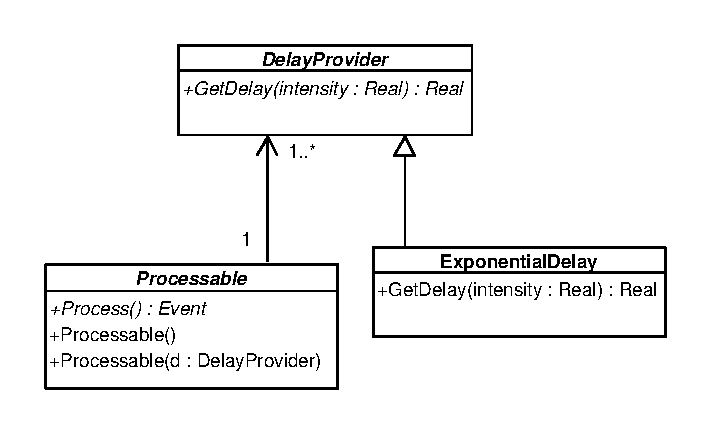
\includegraphics[scale=1]{delayprovider_uml.eps}
	\caption{DelayProvider --- интерфейс для вычисления задержки, который используют элементы системы массового обслуживания}
	\label{delayprovider_uml}
\end{figure}

Для обеспечения среды, которой будет происходит моделирование, а именно --- вестись подсчет прошедшего времени, взаимодействие с реализацией интерфейса Processable и сбор статистики, введен глобальный объект Environment
\begin{figure}[H]
	\centering
	\includegraphics[scale=1]{environment_uml.eps}
	\caption{Глобальный объект Environment}
	\label{environment_uml}
\end{figure}

Статический класс Environment содержит общую для модели информацию --- время моделирования, время конца моделирования и методы, для управления этими параметрами. 
Члены класса Environment будут описаны в последующих разделах.

\begin{figure}[H]
	\centering
	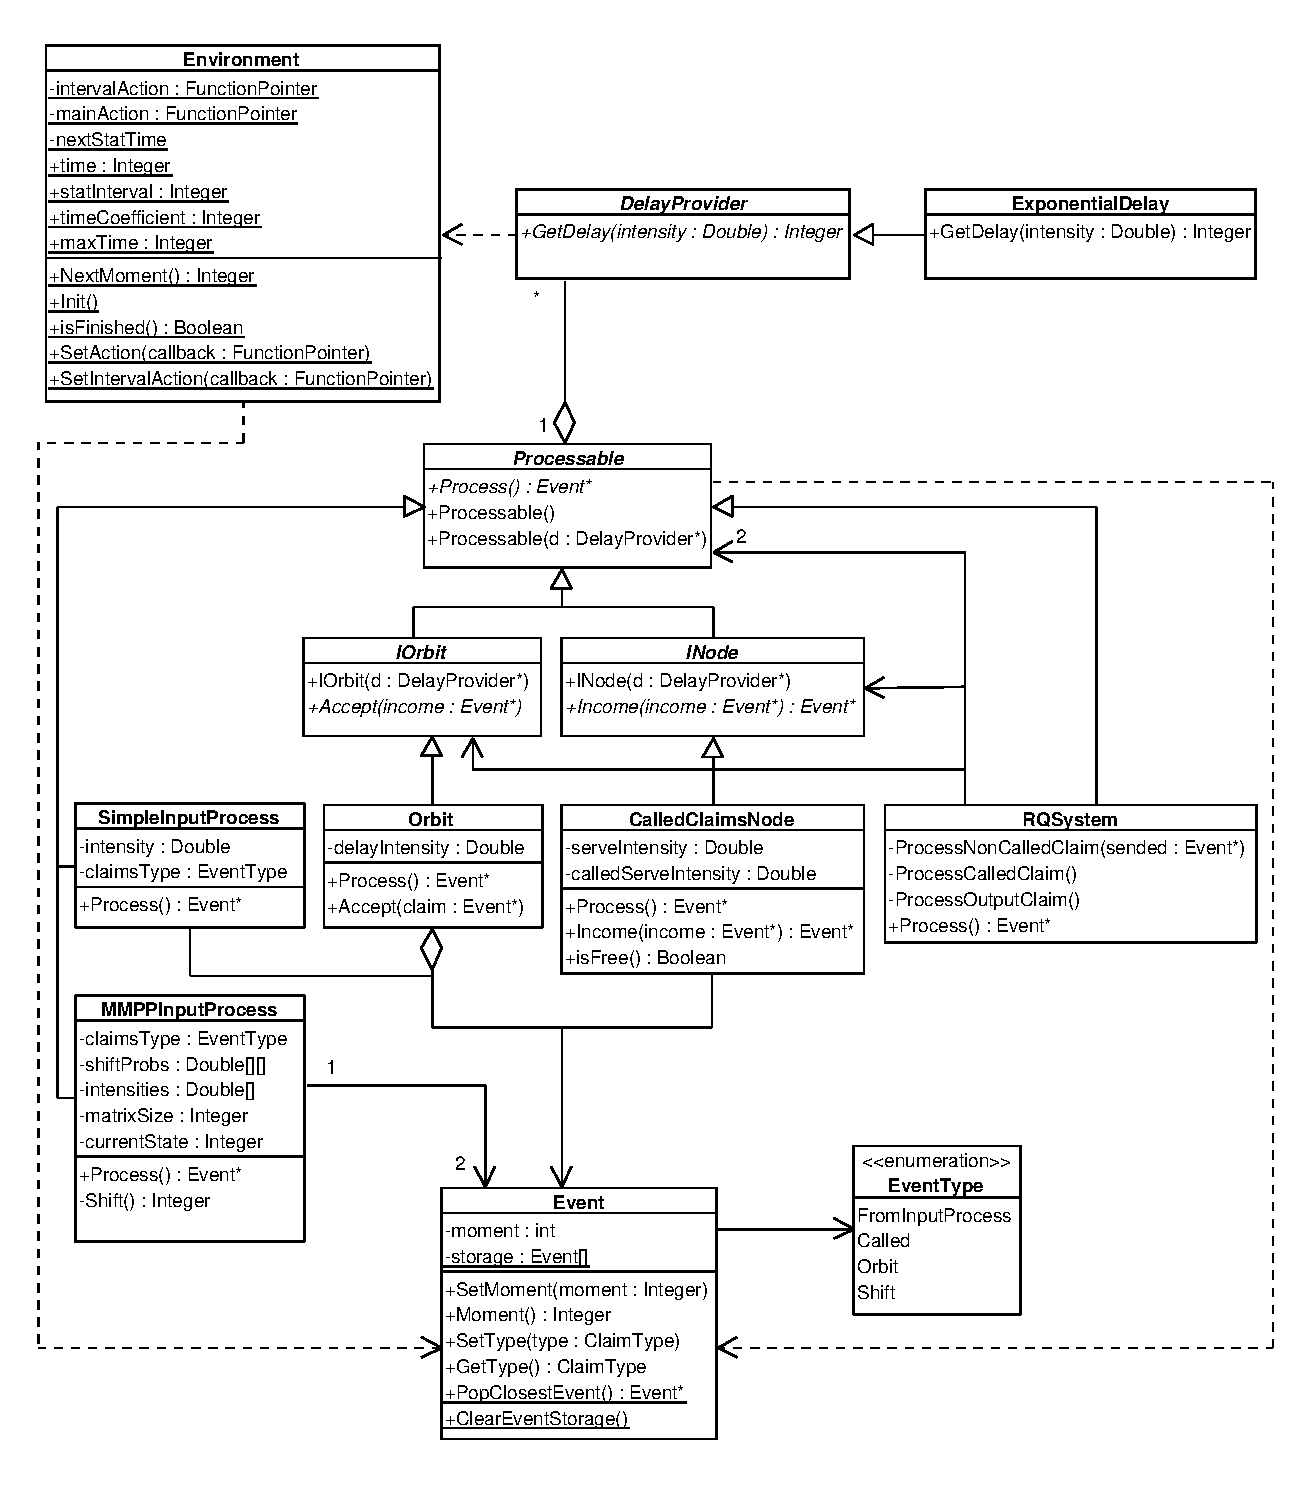
\includegraphics[scale=0.79,width=\textwidth]{domain_uml.eps}
	\caption{Предметная область имитационной модели}
	\label{domain_uml}
\end{figure}
На рисунке \ref{domain_uml} представлена полная предметная область программы. Определенные ранее интерфейсы реализуют конкретные элементы системы, используемые при моделировании. Поскольку, в данной работе рассматривается RQ--система с простейшим и MMPP--потоками, существует две соответствующих реализации входящего потока, подробности функционирования которых будут рассмотрены в следующем разделе. Таким образом, существуют следующие реализации элементов систем массового обслуживания:
\begin{itemize}
	\item Orbit --- реализация источника повторных вызовов, содержащая хранилище заявок (Event), что на диаграмме классов показано агрегацией. Поле delayIntensity хранит интенсивность обращений заявок с орбиты, то есть используется для вычисления экспоненциальной задержки соответствующим объектом DelayProvider.
	\item CalledClaimsNode --- реализация обслуживающего прибора, способная обслуживать два типа заявок --- пришедшие извне и вызванные, для чего служат интенсивности serveIntensity и calledServeIntensity соответственно.
	\item SimpleInputProcess --- реализация простейшего входящего потока, порождающего заявки. Ассоциация с Event показывает, что класс имеет поле с заявкой, которая готовится покинуть источник заявок по истечении задержки.
	\item MMPPInputProcess --- реализация MMPP-потока. Поле shiftProbs хранит матрицу интенсивностей переходов между состояниями, а поле intensities --- интенсивность поступления заявок для каждого состояния. Логика смены состояний находится в приватном методе Shift, где используются поле currentState --- номер текущего состояния, а так же объект Event, в котором хранится момент сменты состояния входящего потока, что на диаграмме показано ассоциацией с множителем 2.
	\item RQSystem представляет агрегирующий класс, где при помощи описанных выше классов строится логика работы системы.
	\item Структура Statistic служит для сбора и подсчета различных характеристик системы в процессе моделирования --- одномерного и двумерного распределения, математического ожидания и др. 
\end{itemize}
\clearpage
\subsection{Процесс моделирования}
В качестве среды для моделирования в реализованной программе выступает глобальный объект Environment, представленный на рисунке \ref{environment_uml}. В процессе моделирования у него вызывается метод NextMoment, который переносит систему в следующий момент моделирования, то есть, совершается одна итерация процесса моделирования. Перед началом моделирования вызывается метод Init, который подготавливает модель к началу работы. Метод isFinished служит для осведомления других участков программы, что моделирование окончено, то есть, что выставленное время моделирования (maxTime) равно текущему (time).

Для обеспечения гибкости действий, которые модель может совершать в процессе работы, метод NextMoment имеет частичную реализацую, в которой вызывается указатель на функцию или лямбда--выражение mainAction. Таким образом, поведение модели можно менять в процессе ее работы, что делает класс Environment универсальным для многих систем, использующих пошаговое моделирование.
\begin{figure}[H]
	\centering
	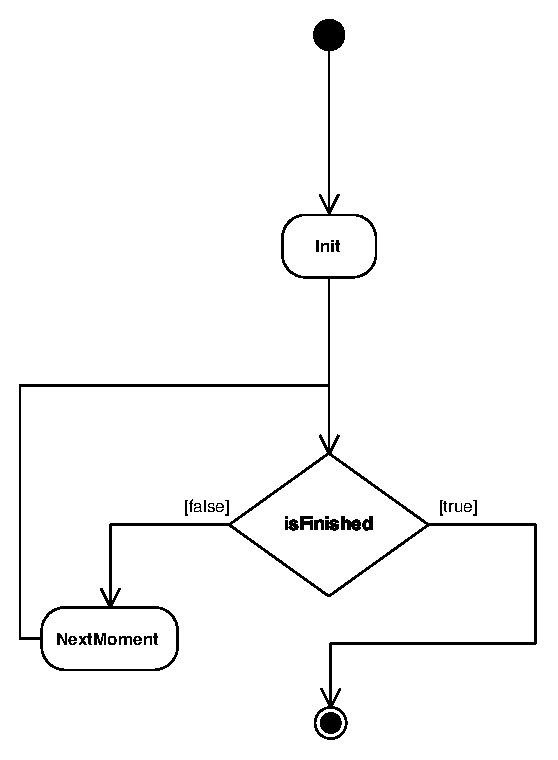
\includegraphics[scale=0.75]{simulation_algo_uml.eps}
	\caption{Общий алгоритм процесса моделирования на основе класса Environment}
	\label{simulation_algo_uml}
\end{figure}

Для сбора статистики и построения распределения вероятностей количества обслуженных заявок в классе Environment предусмотрен механизм интервального сбора данных. Поле statInterval хранит интервал модельного времени, по прошествии которого должен производится вызов функции или лямбда выражения по указателю intervalAction, в котором задается логика сбора данных.

Как видно на рисунке \ref{domain_uml}, класс Environment зависит от класса Event, так как в нем содержится статистическая очередь событий storage, которые вскоре должны произойти в системе. Наглядно это показано на диаграмме последовательностей:
\begin{figure}[H]
	\centering
	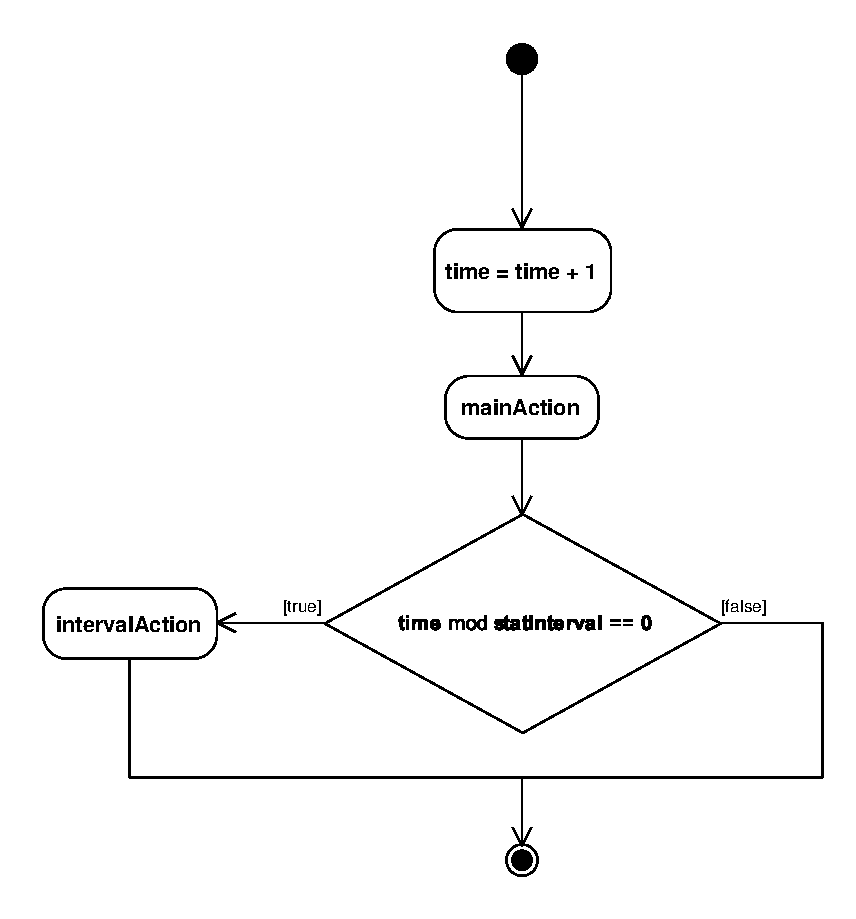
\includegraphics[scale=0.9]{next_moment_algo_uml.eps}
	\caption{Диаграмма последовательностей метода NextMoment}
	\label{next_moment_algo_uml}
\end{figure}
После выполнения mainAction (1.1), из очереди событий извлекается первое предстоящее (1.2). Если такое нашлось, то модельное время перемещается на момент события (1.9). Если это время больше, чем время сбора статистики, то сначала выполняется сбор (1.8), и уже после этого модельное время смещается на момент события. Сбор статистики выполняется в цикле, так как время наступления события может быть больше интервала сбора статистики в несколько раз.
\clearpage
\subsection{Функционирование элементов системы массового обслуживания}
Функционирование же отдельных элементов системы описывается в методах интерфейса Processable и наследуемых от него INode и IOrbit.
Происходящее с обслуживающим прибором во время очередной итерации отражено на диаграммах последовательностей \ref{CalledClaimsNode_Process_uml} и \ref{CalledClaimsNode_Income_uml}
\begin{figure}[H]
	\centering
	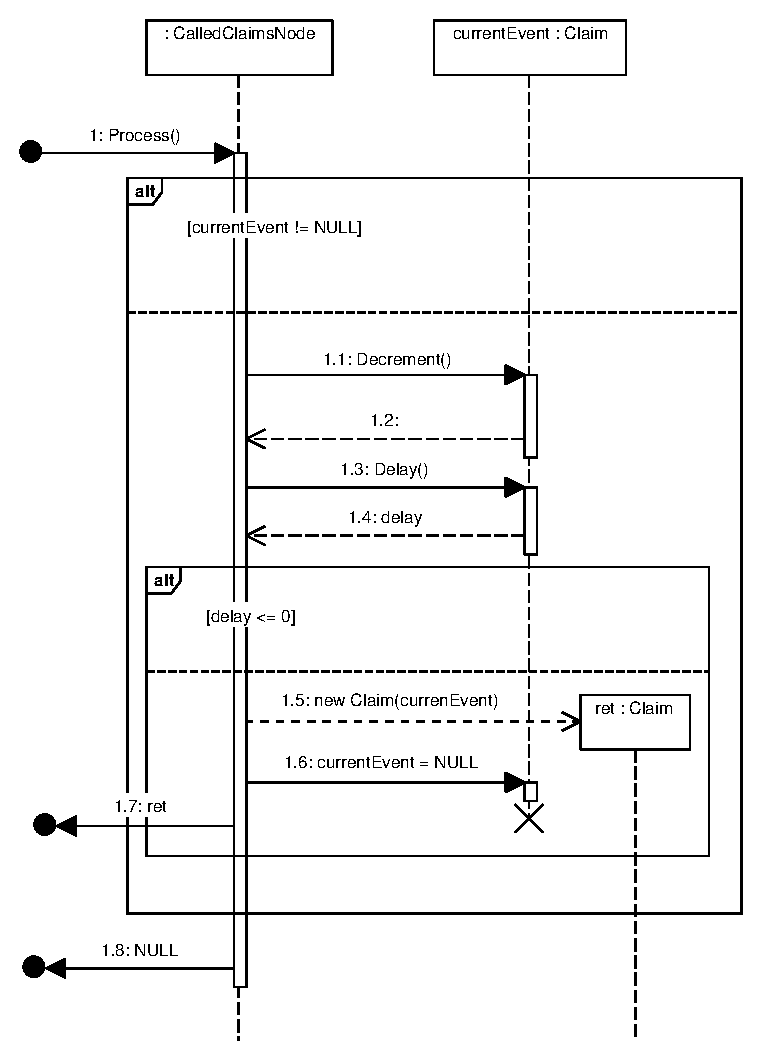
\includegraphics[scale=0.9]{CalledClaimsNode_Process.eps}
	\caption{Диаграмма последовательностей метода Process класса CalledClaimsNode}
	\label{CalledClaimsNode_Process_uml}
\end{figure}
Если прибор на данный момент не обслуживает заявку currentEvent (поле currentEvent на диаграмме \ref{domain_uml} обозначено ассоциацией), то возвращается NULL, говорящий о том, что на данной итерации прибор не закончил обслуживание заявки, так как он либо свободен, либо обслуживание еще продолжается. Иначе, производится проверка, совпадает ли текущее модельное время с моментом наступления события. При совпадении обслуженная заявка уходит с прибора (1.5, 1.6, 1.8).
\begin{figure}[H]
	\centering
	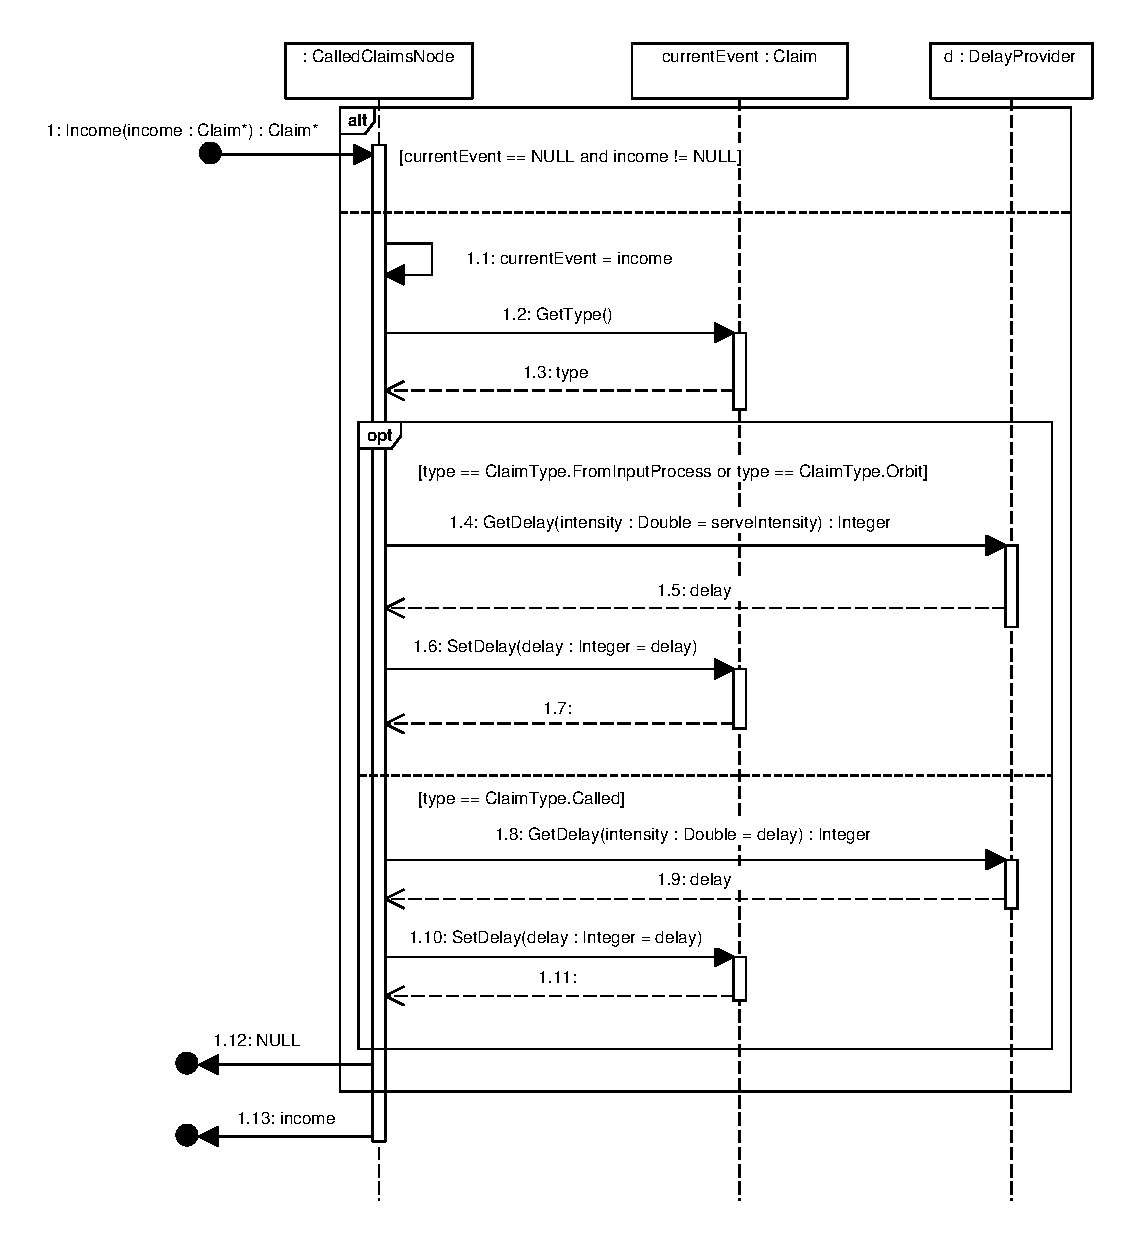
\includegraphics[scale=0.9]{CalledClaimsNode_Income.eps}
	\caption{Диаграмма последовательностей метода Income класса CalledClaimsNode}
	\label{CalledClaimsNode_Income_uml}
\end{figure}
В случае, если пришла заявка, и прибор свободен, пришедшая заявка становится текущей обслуживаемой на приборе (1.1), иначе она возвращается (1.13). В зависимости от типа пришедшей заявки для нее вычисляется время обслуживания --- для заявок с входящего потока и орбиты используется serveIntensity (1.4, 1.6), а для  вызванных используется calledServeIntensity (1.8, 1.10).

Подобный алгоритм, заключающийся в сравнении модельного времени с моментом наступления события, реализован и в других элементах системы.
В методе Accept класса Orbit также вычисляется задержка для пришедшей заявки. После чего она помещается в коллекцию claimStorage, отображенной на диаграмме предметной области (рисунок \ref{domain_uml}) в качестве агрегации. В методе Process (рисунок \ref{Orbit_Process_uml}) производится обход данной коллекции со сравнением времени, когда заявка должна покинуть орбиту, и модельным временем. В случае, если нашлась готовая заявка, она извлекается (1.5) из коллекции и возвращается (1.6).
 \begin{figure}[H]
 	\centering
 	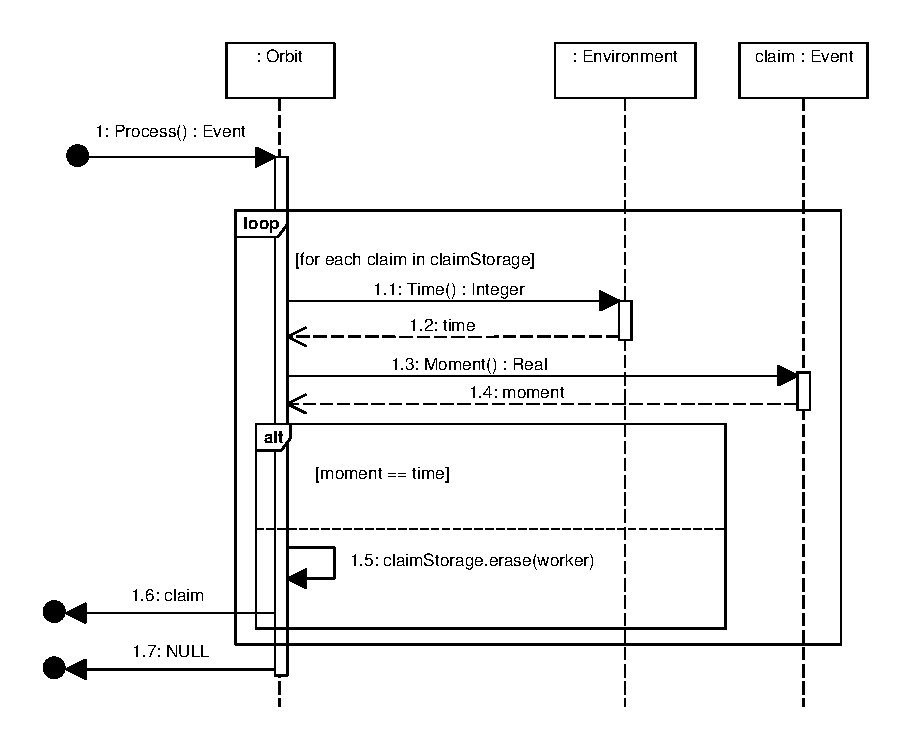
\includegraphics[scale=0.9]{Orbit_Process.eps}
 	\caption{Диаграмма последовательностей метода Process класса Orbit}
 	\label{Orbit_Process_uml}
 \end{figure}
Тот же подход используется для метода Process классов SimpleInputProcess и \\ MMPPInputProcess. Более подробного рассмотрения требует алгоритм смены состояния управляющей цепи MMPP--потока, реализованного в методе Shift класса MMPPInputProcess.

Как было показано в главе \ref{mmpp_section}, время нахождения в одном из состояний и вероятность перехода в другое для MMPP-потока определяется матрицей инфинитезимальных характеристик $Q$
\begin{equation*}
	\boldsymbol{Q}=\begin{bmatrix}
		q_{11} &  \dots &  q_{1n}\\
		\vdots & \ddots &  \\
		q_{n1} &    	&	q_{nn}
	\end{bmatrix}
\end{equation*}
Интенсивностью, на основе которой вычисляется задержка управляющей цепи в $i$--ом состоянии является диагональный элемент матрицы $-q_{i,i}$, а вероятностью перехода из $i$--ого состояния в $j$--ое является выражение $\frac{q_{i,j}}{-q_{i,i}}$.В таком случае, при наступлении события смены состояния выполняется следующий алгоритм
   \begin{figure}[H]
  	\centering
  	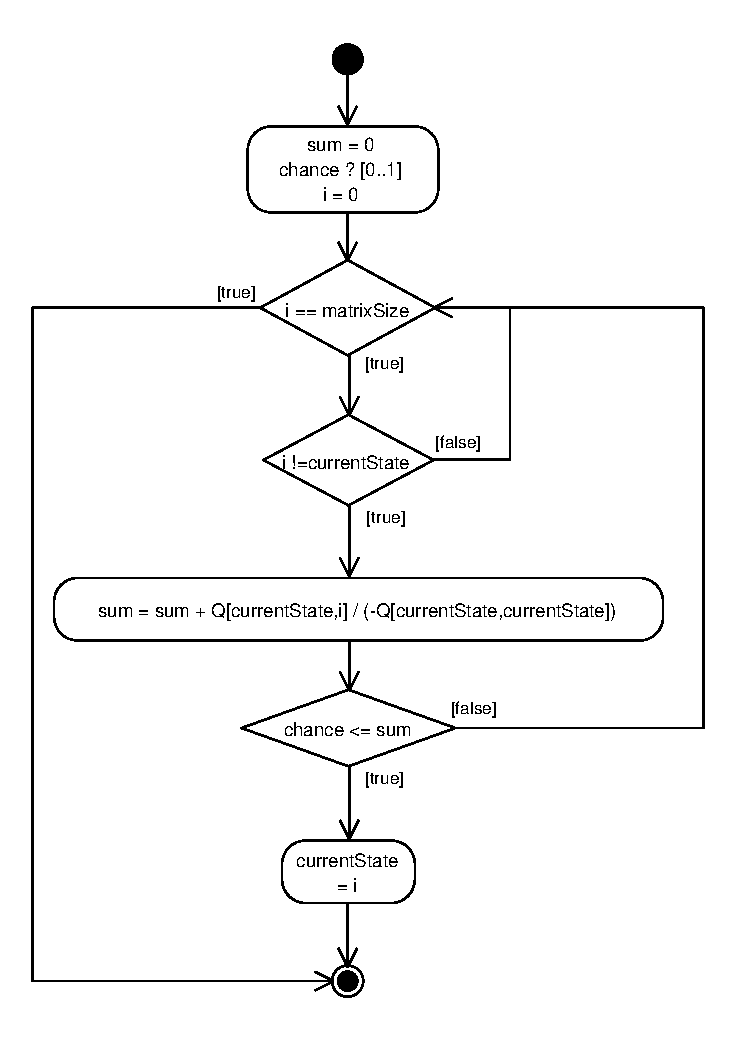
\includegraphics[scale=0.7]{shift_algo.eps}
  	\caption{Алгоритм смены состояния MMPP--потока}
  	\label{shift_algo_uml}
  \end{figure}
В начале работы вычисляется случайная величина chance, определяется переменная sum для суммирования вероятностей по строке матрицы $Q$ и счетчик цикла i. Цикл идет по строке текущего состояний currentState. В случае, если текущий элемент строки недиагональный, к sum прибавляется вероятность попадания в состояние i, после чего производится проверка, больше ли величина sum случайной величины chance. Графически это представляется таким образом, что точка chance принадлежит отрезку $[0,sum]$, а прибавленная к sum на текущей итерации вероятность попадания управляющей цепи в состояние i обеспечила принадлежность точки к отрезку, следовательно, прибор принимает состояние i. После этого время нахождения управляющей цепи в нем рассчитывается с помощью метода GetDelay интерфейса DelayProvider.
\clearpage
\subsection{Интерфейс и работа программы}
Для начала работы с программой, в первую очередь, необходимо задать параметры моделирования. Среди них:
\begin{itemize}
	\item Время моделирования (Time limit). Данные единицы являются условными и используются в качестве модельного времени.
	\item Тип входящего потока (Input Process).
	\item Интенсивность входящего потока (Simple input). Для MMPP--потока матрица инфинитезимальных характеристик и вектор интенсивностей задается в модельном окне.
	\item Интенсивность вызова заявок прибором (Calling intensity).
	\item Интенсивность обслуживания входящих и вызванных заявок (Serving intensity, Called serving intensity).
	\item Интервал сбора статистики для построения распределения вероятностей (Moment T). Так же выражен в единицах модельного времени.
\end{itemize}
   \begin{figure}[H]
	\centering
	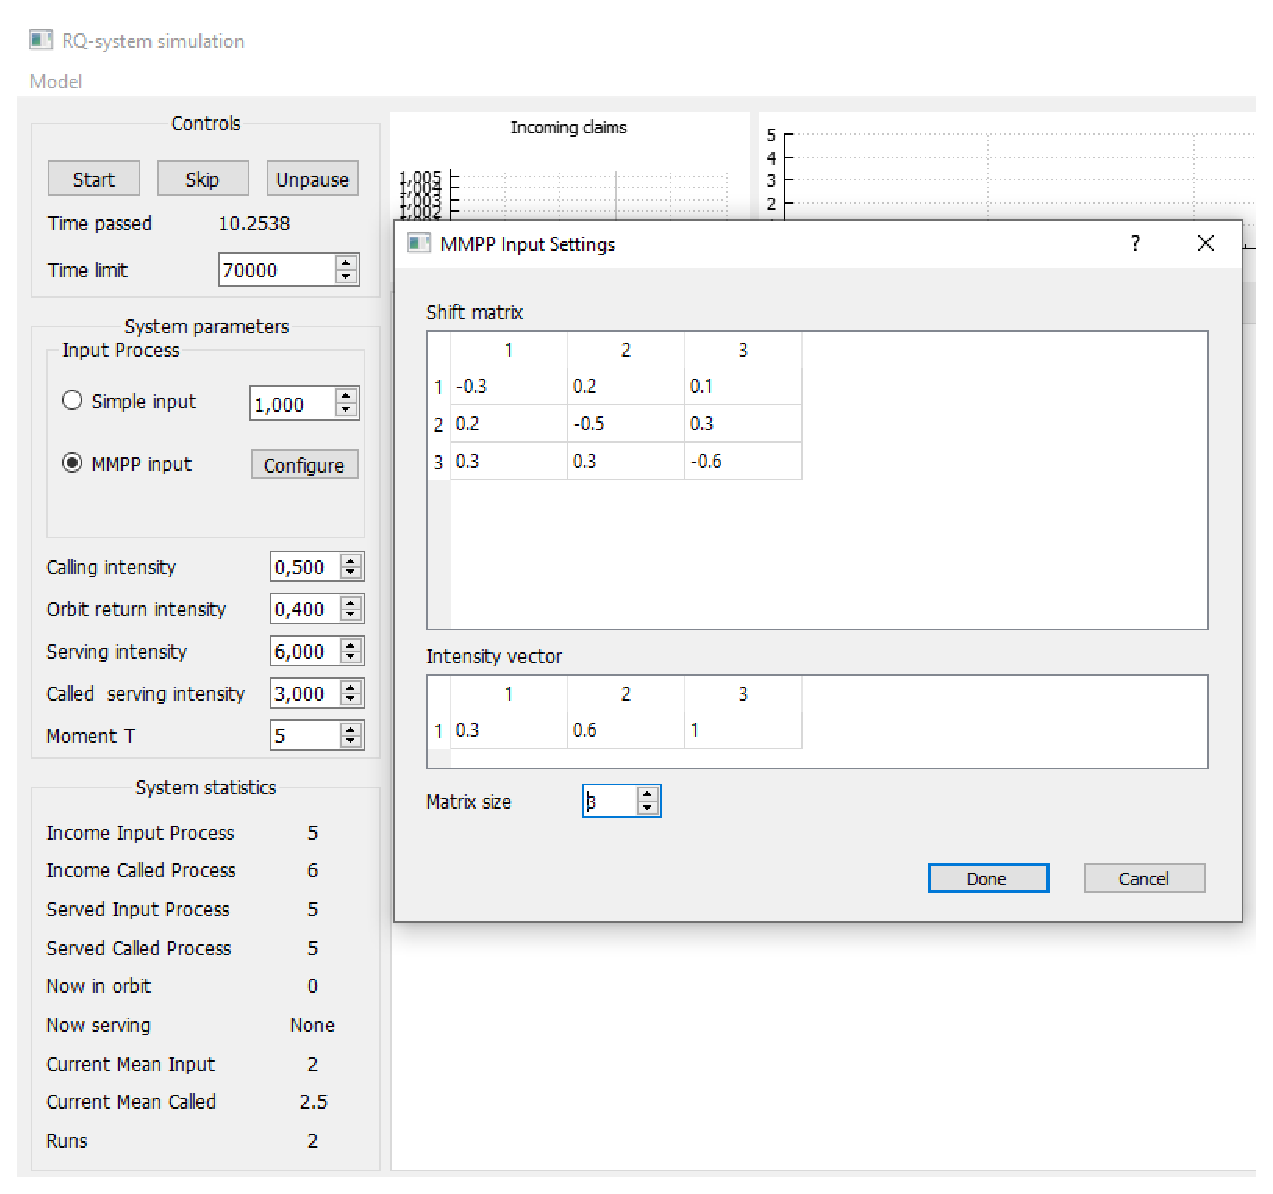
\includegraphics[scale=0.5]{interface_params.eps}
	\caption{Задание параметров моделирования}
	\label{interface_params}
\end{figure}
Управление процессом моделирования выполняется с помощью специальной области Controls (рисунок \ref{interface_params}). Кнопка Start сбрасывает результаты предыдущего запуска модели и начинает моделирование заново с установленными параметрами.
\subsubsection{Моделирование в реальном времени}
Реализация программы предусматривает два варианта работы с моделью. В первом случае, пользователь имеет возможность в реальном времени наблюдать, как меняется состояние системы с помощью визуализации распределения вероятностей числа обслуженных заявок и других характеристик на графиках и в области System statistics, а также приостанавливать моделирование с помощью кнопки Pause, которая так же служит и для возобновления процесса моделирования. Данный подход реализован с помощью таймера, при каждом тике которого выполняется очередная итерация моделирования. Для настройки длины интервала таймера используется модальное окно конфигурации:
\begin{figure}[H]
	\centering
	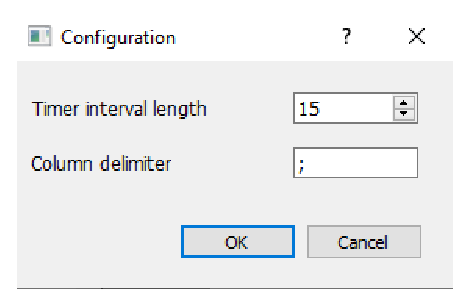
\includegraphics[scale=0.7]{interface_config.eps}
	\caption{Модальное окно конфигурации}
	\label{interface_config}
\end{figure}
Измененные пользователем настройки сохраняются в файле конфигурации для использования их в последующих запусках программы. Предназначение второго параметра будет описано в следующих разделах.

   \begin{figure}[H]
	\centering
	\includegraphics[scale=0.5,width=\textwidth]{interface_realtime.eps}
	\caption{Моделирование работы системы в реальном времени}
	\label{interface_realtime}
\end{figure}
Как видно на рисунке \ref{interface_realtime}, в момент, когда в системе наступает очередное событие, то есть, ее состояние меняется, производится сбор статистики и ее показ в реальном времени. Основная статистика работы модели показана в области System statistics, которая содержит следующую информацию:
\begin{itemize}
	\item Количество пришедших заявок входящего потока (Income Input Process).
	\item Количество заявок, вызванных прибором (Income Called Process).
	\item Количество обслуженных заявок входящего потока (Served Input Process).
	\item Количество обслуженных вызванных прибором заявок (Served Called Process).
	\item Количество заявок на орбите в данный момент (Now in orbit).
	\item Тип в данный момент обслуживаемой заявки (Now serving).
	\item Математическое ожидание обслуженных заявок входящего потока (Current Mean Input).
	\item Математическое ожидание обслеженных вызванных прибором заявок (Current Mean Called).
	\item Количество сборов статистики, интервал которых задан параметром Moment T (Runs).
\end{itemize}
Поскольку математическое ожидание вычисляется на основе полученного на данный момент распределения вероятности, обновление полей Current Mean Input и Current Mean Called происходит с интервалом Moment T. Для отображения области System statistics используется ранее упомянутая структура Statistic (рисунок \ref {domain_uml}), которая служит для накопительного сбора статистики и подсчета распределения и математического ожидания. 

Помимо текстового представления, изменение состояния системы отражено на графиках. Левый верхний график отображает моменты поступления заявок входящего потока. По оси X отсчитывается модельное время.
   \begin{figure}[H]
	\centering
	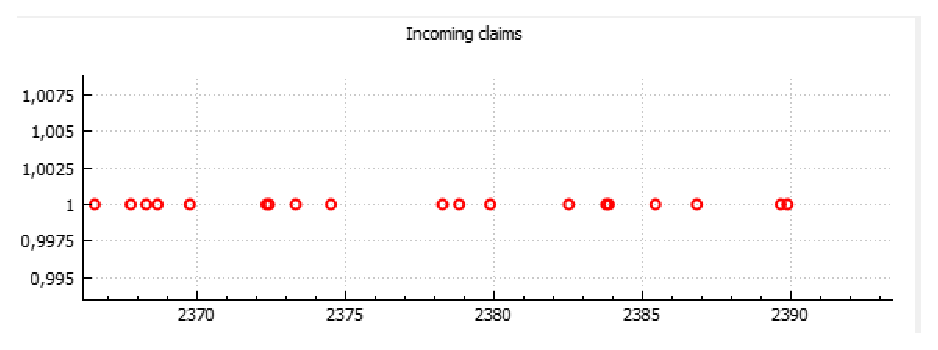
\includegraphics[scale=0.7]{incoming_claims.eps}
	\caption{Отображение времени прихода заявок в систему на графике}
	\label{interface_incoming_claims}
\end{figure}
Правый верхний график отображает изменение количества заявок на орбите в случае моделирования системы с простейшим входящим потоком и историю изменения состояния управляющей цепи MMPP--потока при моделировании системы с MMPP--потоком. По оси X для обоих графиков отсчитывается модельное время. По оси Y количество заявок на орбите, либо состояние управляющей цепи.

   \begin{figure}[H]
	\centering
	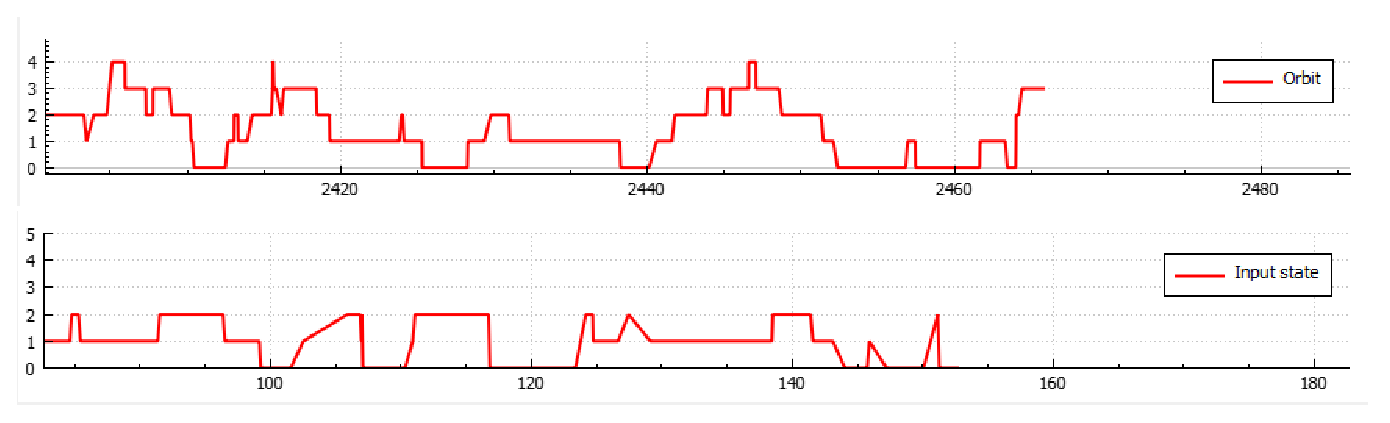
\includegraphics[scale=0.8,width=\textwidth]{orbit_mmppState.eps}
	\caption{Отображение изменения размера орбиты (верхний) и состояния управляющей цепи (нижний) на графике}
	\label{interface_orbit_mmpp}
\end{figure}
Графики на рисунках \ref{interface_incoming_claims} и \ref{interface_orbit_mmpp} имеют опцию масштабирования к выделенной пользователем области.
\subsubsection{Ускоренное моделирование }
Второй вариант работы с программой предполагает, что пользователю требуется быстро получить результаты моделирования. Для этого служит кнопка Skip в области Controls, при нажатии которой таймер останавливается, и производится моделирование системы до установленного времени в цикле. В таком случае, программа отобразит модальное окно, уведомляющее пользователя, что на данный момент выполняется моделирование, блокируя основное.
 \begin{figure}[H]
	\centering
	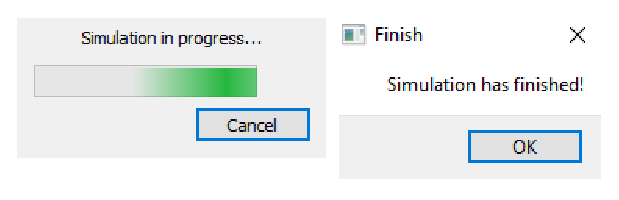
\includegraphics[scale=0.84]{interface_skip.eps}
	\caption{Модальные окна уведомления пользователя о статусе процесса моделирования}
	\label{interface_skip}
\end{figure}
По завершении моделирования отображаемая статистика и главный график обновляются в соответствии с актуальными результатами. По нажатии кнопки отмены (Cancel) в модальном окне статуса моделирования цикл закончит свою работу, а таймер возобновит отсчет. Таким образом, программа продолжит моделирование в реальном времени.  
\subsubsection{Работа с главным графиком}
Важнейшую информацию о работе системы отображает главный график, занимающий наибольшую рабочую область окна. На нем отображается текущее двумерное распределение вероятностей числа обслуженных заявок входящего потока и вызванных заявок в виде трехмерных столбцов. Распределение обновляется в момент модельного времени, кратный параметру Moment T. По осям X и Y отложены количество обслуженных заявок входящего потока и вызванных заявок соответственно.
\begin{figure}[H]
	\centering
	\includegraphics[scale=0.8,width=\textwidth]{interface_mainplot.eps}
	\caption{Отображение распределения вероятности на главном графике}
	\label{interface_mainplot}
\end{figure}
Рабочая область графика позволяет проводить предварительный анализ работы системы. В первую очередь график поддерживает масштабирование и перемещение в пространстве отображаемой области с помощью мыши, клавиатуры и слайдеров поворота камеры относительно графика по горизонтали (Rotate horizonatally) и вертикали (Vertical Rotation).  Также, пользователь имеет возможность выделить любой столбец на графике для получения о нем подробной информации. Помимо этого, кнопка Zoom to selected bar при нажатии позволяет масштабировать и переносить камеру к выбранному столбцу автоматически.
\begin{figure}[H]
	\centering
	\includegraphics[scale=0.8,width=\textwidth]{interface_plot_selection.eps}
	\caption{Перенос камеры к выбранному столбцу}
	\label{interface_plot_selection}
\end{figure}
Выделение участков графика реализовано в различных вариациях:
\begin{itemize}
	\item Выделение столбца
	\item Выделение ряда
	\item Выделение ряда и столбца, так же, с подробной информацией о выделенном столбце
	\item Перекрестное выделение рядов
	\item Перекрестное выделение рядов с выделением столбца
	\item Срез по ряду
	\item Срез по ряду с выделением столбца
\end{itemize}
В отличие от других вариантов выделения, при выборе среза выделенного ряда строится дополнительная область, в которой выбранный ряд отображен в качестве отдельного графика. По нажатии на трехмерное представление графика в левом верхнем углу, выделение сбрасывается.
\begin{figure}[H]
	\centering
	\includegraphics[scale=0.8,width=\textwidth]{interface_plot_selection_slice.eps}
	\caption{Выделение с построением среза по выбранному ряду и столбцу}
	\label{interface_plot_selection_slice}
\end{figure}
Для удобной работы с визуальной точки зрения, трехмерный график предусматривает настройку отображения графических элементов. Так, пользователь может изменять видимость фона (Show background), сетки (Show grid), отражений поверхностей (Show reflections). Имеется возможность смены  цветовой схемы (Change theme), шрифта (Change font), размера шрифта (Font size) и поворота ярлыков (Label Rotation). 

\begin{figure}[H]
	\centering
	\includegraphics[scale=0.6]{interface_plot_custom.eps}
	\caption{Настройка отображения основного графика}
	\label{interface_plot_custom}
\end{figure}

Также, помимо двумерного распределения вероятностей числа обслуженных заявок, пользователь может наблюдать распределение вероятностей суммарного числа обслуженных заявок на вкладке Summary основного графика. Это представление так же, как и другие графики в программе, имеют опцию масштабирования к выделенной области. Переключение между двумя представлениями распределения вероятностей может выполняться пользователем в любой момент работы программы за исключением времени, когда производится ускоренное моделирование. 
\begin{figure}[H]
	\centering
	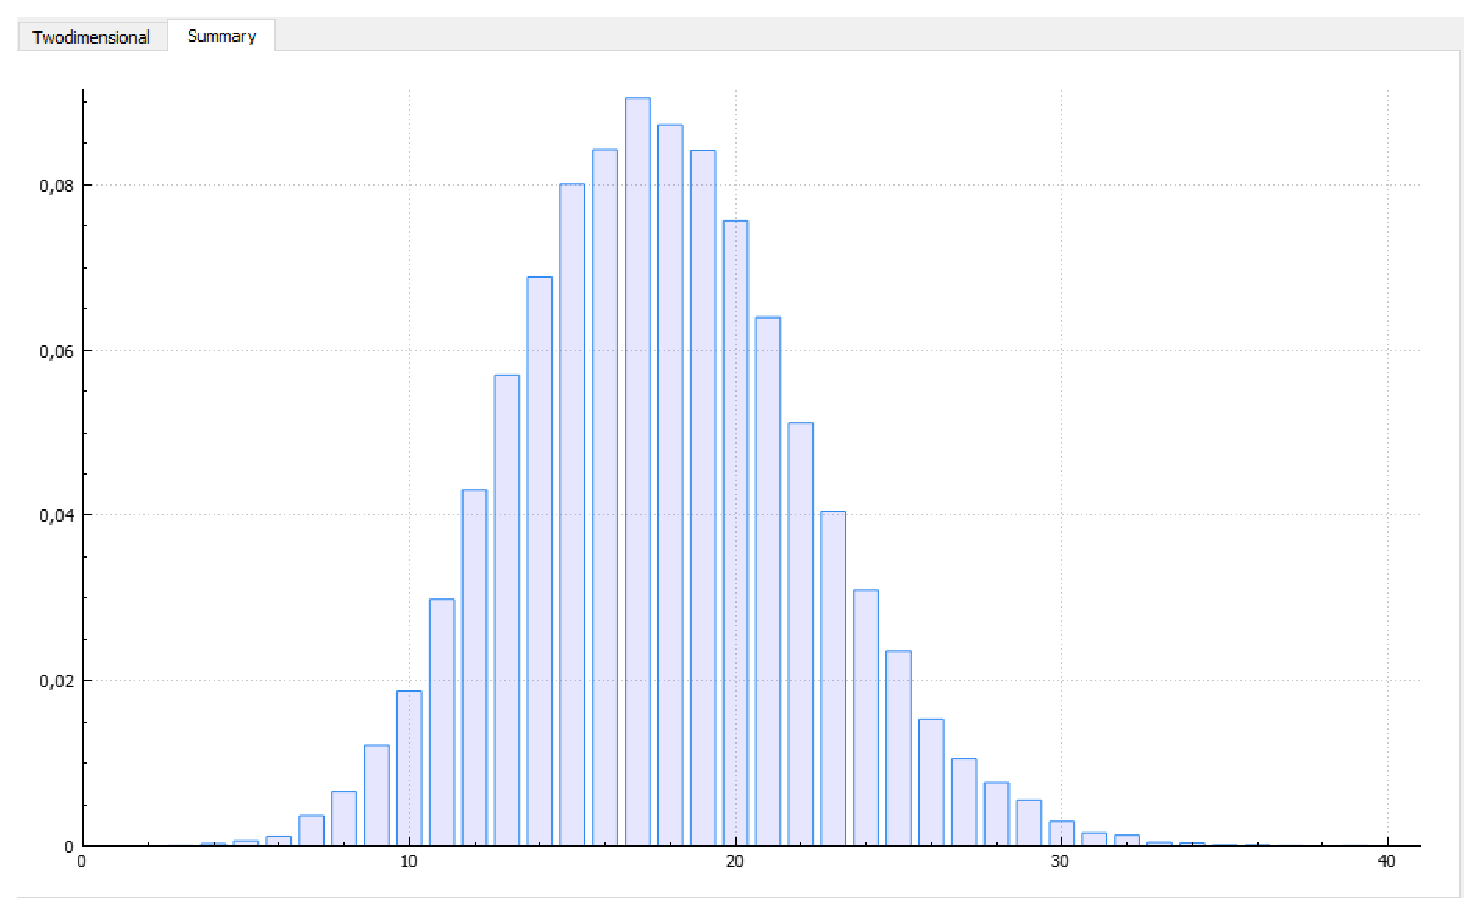
\includegraphics[scale=0.8,width=\textwidth]{interface_mainplot_summary.eps}
	\caption{Вкладка основного графика, отображающая распределение вероятностей суммарного числа обслуженных заявок}
	\label{interface_mainplot_summary}
\end{figure}
\subsubsection{Экспорт результатов моделирования}
В меню Model основного окна имеется опция экспорта в текстовый файл текущего распределения вероятностей числа обслуженных заявок в двумерном виде и суммарном.
\begin{figure}[H]
	\centering
	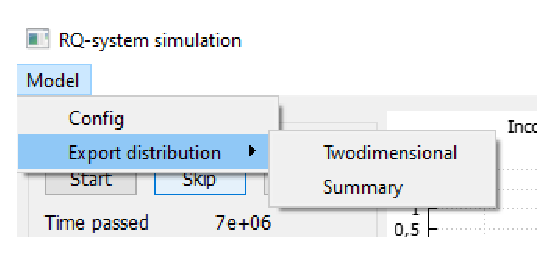
\includegraphics[scale=0.8]{interface_export.eps}
	\caption{Опции экспорта}
	\label{interface_export}
\end{figure}
При выборе опции Summary распределение будет записано в файл формата CSV, где каждое значение будет с новой строки. При выборе опции Twodimensional распределение будет записано в виде таблицы с разделителем, установленным пользователем в окне конфигурации (рисунок \ref{interface_config}). По умолчанию разделителем является символ \textquote{;}. Поскольку формат CSV является основным при работе с данными ввиду удобного табличного представления с помощью разделителей, импортировать и использовать полученные при моделировании данные можно в широком спектре программного обеспечения. Для анализа численных результатов в данной работе используется система компьютерной алгебры Mathcad.
\begin{figure}[H]
	\centering
	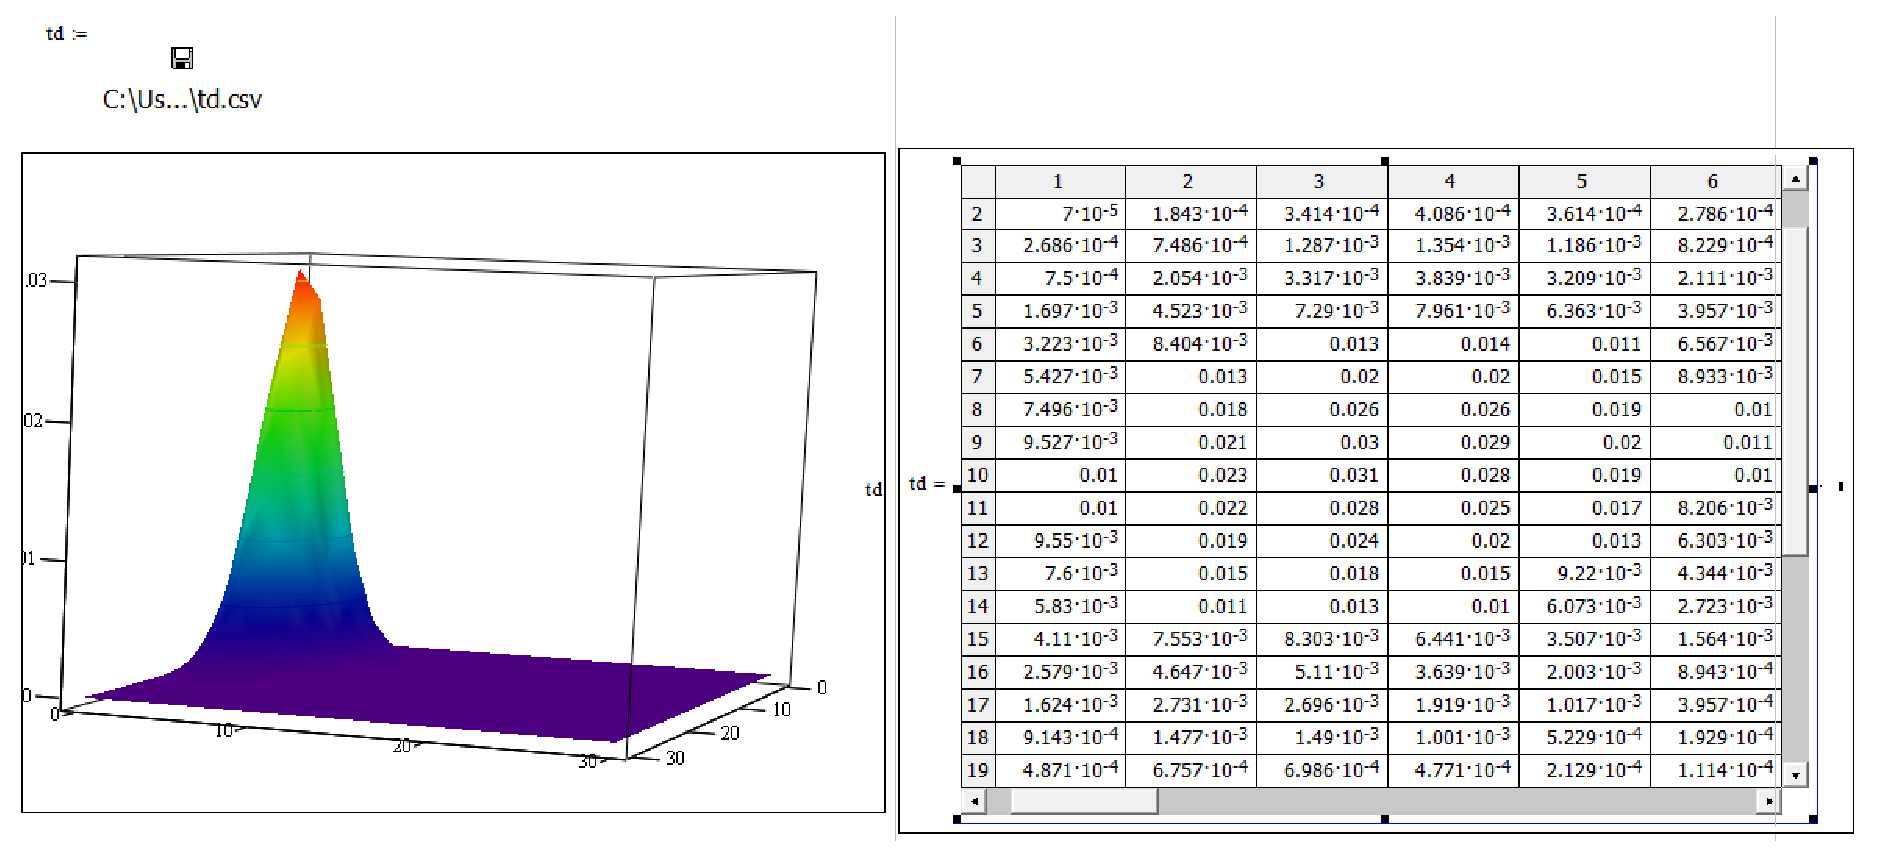
\includegraphics[width=\textwidth]{interface_export_mathcad.eps}
	\caption{Результаты моделирования, импортированные в среду Mathcad}
	\label{interface_export_mathcad}
\end{figure}
На рисунке \ref{interface_export_mathcad} представлена плоскость двумерного распределения вероятностей числа обслуженных заявок (слева) и таблица распределения (справа), полученные в результате моделирования и импорта в среду Mathcad.
\clearpage

\subsection{Особенности реализации}
Реализация предметной области программы выполнена на языке программирования C++ стандарта 2017 года (C++1z). Оболочка программы и графический интерфейс были выполнены на базе фреймворка для разработки кроссплатформенного программного обеспечения QT \cite{QtDoc}. Таким образом, представленная программа является кроссплатформенной, то есть, может быть собрана для работы в операционных системах GNU/Linux, Microsoft Windows и macOS. Выбор в сторону разработки на C++ был сделан, в первую очередь, из--за низкоуровневого программирования, которое позволяет писать эффективный код и более точно распоряжаться используемыми ресурсами системы. По этой же причине, C++ отлично подходит для работы с графикой. Также, в C++ поддерживается объектно--ориентированный подход к программированию, что важно для реализации ранее описанной предметной области программы.
\\\\
Минимальные системные требования для работы программы:
\begin{itemize}
	\item Процессор с тактовой частотой 1.8 ГГц и выше.
	\item Оперативная память емкостью 2 Гб и больше.
	\item Видеоадаптер и монитор VGA с разрешением 1280 х 1024 и выше.
	\item 50 Мб свободного места на диске
	\item Клавиатура и мышь
	\end{itemize}

\subsubsection{Генерация псевдослучайных чисел}
Поскольку генераторы псевдослучайных чисел во многих языках программирования, в том числе, в C++ генерируют новые значения на основе системного времени или такта процессора, возникает проблема повторения последовательности значений при частой генерации, например, в цикле. А поскольку для расчета экспоненциальной задержки каждого события в модели используется генерация случайных чисел, возникновение этой проблемы неизбежно.

Решением проблемы стало использование вихря Мерсенна --- генератора псевдослучайных чисел, основывающимся на свойствах простых числе Мерсенна. Данный генератор лишен многих недостатков других генераторов, таких как предсказуемость, малый период и легко выявляемые статистические закономерности.

В С++ данный алгоритм имеет реализацию под названием MT19937 и содержится в стандартной библиотеке, начиная со стандарта C++11. Его период составляет $2^{19937}$, чего с излишком хватит для продолжительного процесса моделирования. 

В коде использование вихря Мерсенна представлено следующим образом
\begin{lstlisting}
#include <random>

std::random_device rd;
std::mt19937 gen(rd());
std::uniform_real_distribution<double> distribution(0,1);

double NextDouble()
{
	return distribution(gen) ;
}
\end{lstlisting}

\subsubsection{Отображение статуса при ускоренном моделировании}
При ускоренном моделировании возникает проблема отображения статуса моделирования без блокировки основа потока, в котором производится отрисовка графического интерфейса. Проблема заключается в том, что цикл, в котором производится моделирование системы блокирует отрисовку графического интерфейса до окончания его работы, а все объекты графического интерфейса должны находится в основном потоке программы, что исключает создание параллельного потока для отрисовки. Так, пользователь не может удостовериться, что программа продолжает свою работу, ибо процесс перестает отвечать на сигналы операционной системы.
\begin{lstlisting}
class MainWindow : public QMainWindow
{
	...
	private:
	...
	QFutureWatcher<void> watcher;
	...
};
\end{lstlisting}
\begin{lstlisting}
void MainWindow::skip()
{
 if(Environment::Time()>0  && !Environment::isFinished()){
 ...
 timer->stop();
 skipping = true;
 QFuture<void> future = QtConcurrent::run([this]{
	while (!Environment::isFinished() && skipping){
		Environment::NextMoment();
	}
 });
 watcher.setFuture(future);
 progressDialog.exec();
 }
}
\end{lstlisting}

Для решения данной проблемы был использован специальный инструмент фреймворка QT --- QTConcurrent, предназначенный для параллельного запуска ресурсоёмких задач. Так, основной поток будет занят отрисовкой статуса моделирования (рисунок \ref{interface_skip}), а моделирование будет происходить асинхронно, что положительно скажется на быстродействии.
\begin{lstlisting}
connect(&watcher,&QFutureWatcher<void>::finished,this,[=](){
	progressDialog.close();
	updateTime();
});
\end{lstlisting}
Для уведомления модального окна об окончании цикла моделирования служит объект QFutureWatcher, который осуществляет привязку события завершения работы потока к лямбда--функции, в которой производится закрытие окна статуса и обновление отображаемой статистики.
\clearpage %Имитационное моделирование
\section{Численные эксперименты}
\subsection{Проверка стабильности имитационной модели}
Для начала проведения численного анализа полученных асимптотических результатов необходимо проверить точность работы реализованной имитационной модели. Для проверки, запустим модель несколько раз с одинаковыми параметрами и для полученных результатов вычислим критерий согласия Колмогорова. Критерий согласия Колмогорова (расстояние Колмогорова) предназначен для проверки гипотезы о том, что некое эмпирическое распределение, в данном случае, распределение, построенное в ходе работы имитационной модели, соответствует предполагаемой модели, которая, в данном случае, так же является результатом работы имитационной модели.

Расстояние Колмогорова вычисляется по следующей формуле
\begin{equation*}
	\Delta = \underset{0 \leq i \leq \infty}{max}\bigg\rvert \sum_{v=0}^{i} (P_0(v) - P_1(v))\bigg\rvert
\end{equation*}
Для численного анализа в данной работе применяется система компьютерной алгебры Mathcad. В ней были построены графики распределения вероятностей и вычислено расстояния Колмогорова для двух запусков имитационной модели с одинаковыми параметрами системы

Введем следующие обозначения: $\Delta_S$ --- расстояние Колмогорова для суммарного распределения вероятностей, $\Delta_{TD}$ --- расстояние Колмогорова для двумерного распределения. Данные обозначения будут использоваться в дальнейших экспериментах.

\begin{figure}[H]
	\centering
	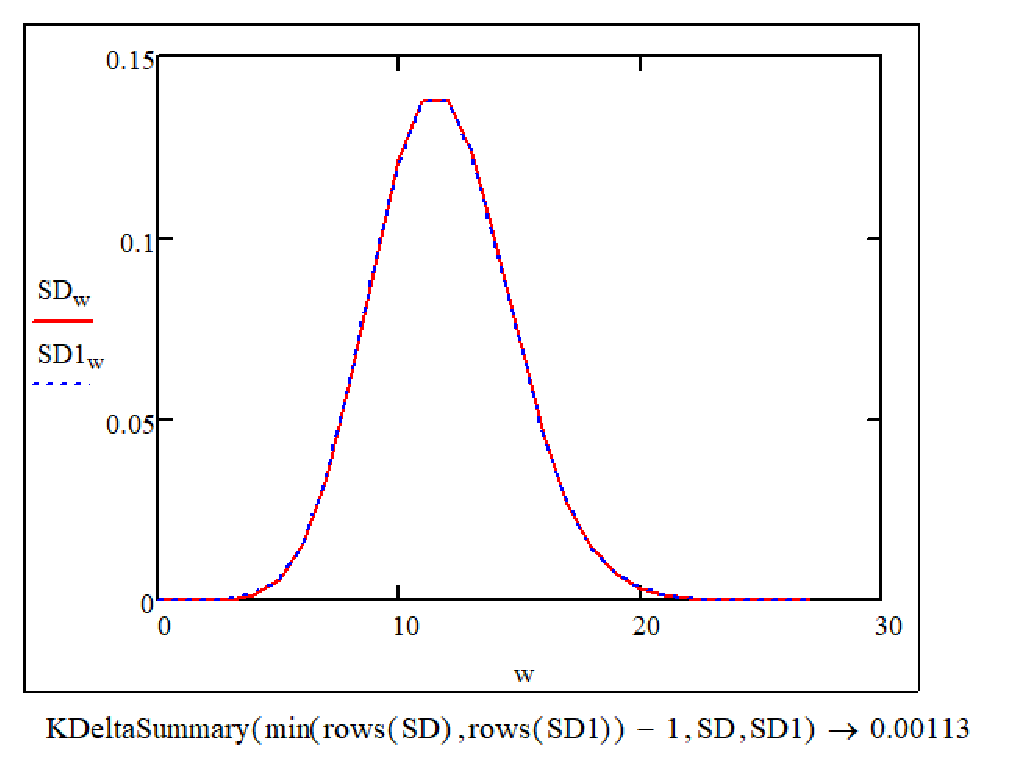
\includegraphics[scale=0.5]{mathcad_check_sim.eps}
	\caption{Сравнение двух отдельных запусков имитационной модели с простейшим входящим потоком}
	\label{experiments_kol_dist_sim}
\end{figure} 

На рисунке \ref{experiments_kol_dist_sim} представлено сравнение двух запусков имитационной модели с параметрами системы: $\lambda = 1, \alpha = 0.5, \sigma = 0.4, \mu_{1} = 6, \mu_{2} = 3, t = 10 $. Запуски модели дали практически одинаковые результаты. Графики рядов распределения вероятностей полностью накладываются друг на друга, а расстояния Колмогорова составили

\begin{equation*}
	\Delta_S = 0.0007,\\
	\Delta_{TD} = 0.0008.
\end{equation*}

Данный эксперимент был проведен и для системы с входящим MMPP--потоком. Были заданы следующие параметры: $\alpha = 0.5, \sigma = 0.4, \mu_{1} = 6, \mu_{2} = 3, t = 10 $,
\begin{equation*}
	\boldsymbol{Q}=\begin{bmatrix}
		-0.3 &  0.1 &  0.2\\
		0.2 & -0.5 &  0.3\\
		0.3 &  0.3 &  -0.6
	\end{bmatrix}
\end{equation*}
\begin{equation*}
	\boldsymbol{\Lambda}=\begin{bmatrix}
		1 &	0 & 0\\
		0 &	0.6 & 0\\
		0 &	0 & 0.7\\
	\end{bmatrix}.
\end{equation*}

Результаты эксперимента представлены на рисунке \ref{experiments_kol_dist_sim2}

\begin{figure}[H]
	\centering
	\includegraphics[scale=0.5,width=\textwidth]{mathcad_check_sim2.eps}
	\caption{Сравнение двух отдельных запусков имитационной модели с MMPP--потоком}
	\label{experiments_kol_dist_sim2}
\end{figure} 

Графики плотности распределений также полностью накладываются друг на друга, расстояния Колмогорова составили

\begin{equation*}
	\Delta_S = 0.0009,\\
	\Delta_{TD} = 0.0018.
\end{equation*}

Тестирование имитационной модели проводилось с заданным временем моделирования $7\cdot 10^6$. Было выбрано именно такое значение параметра, так как оно дает наивысшую точность, то есть, при установке значение ниже указанного, точность начинает снижаться, а при повышении ее улучшения не наблюдается. Ниже в таблице \ref{time_dynamics} приведена динамика изменения точности запусков модели при одинаковых параметрах в зависимости от заданного времени моделирования. Максимальное время моделирование, которое допускает реализация программы --- $10^7$. Параметры системы соответствуют параметрам из эксперимента на рисунке \ref{experiments_kol_dist_sim}.

\begin{table}[h!] 
	\centering
	\caption{Расстояние Колмогорова при различных значениях параметра времени моделирования}
	\label{time_dynamics}
	\begin{tabular}{| c | c | c | c | c | c |} 
		\hline
		$t$ & $5\cdot 10^4$ & $10^6$ & $5\cdot 10^6$ & $7\cdot 10^6$ & $10^7$\\ 
		\hline
		$\Delta_S$ & 0.011 & 0.0023 & 0.0016 & 0.0007 & 0.0008\\
		\hline
		$\Delta_{TD}$ & 0.0176 & 0.0034 & 0.0022 & 0.0008 & 0.0012\\
		\hline
	\end{tabular}
\end{table} 

Исходя из вышеописанных экспериментов, можно сделать вывод, что реализованная имитационная модель дает стабильные результаты, что подтверждают вычисленные значения расстояния Колмогорова для обоих видов распределений --- его значение не превышает порог в $10^{-3}$. Следовательно, модель может быть применена для анализа и оценки применимости асимптотических результатов с указанной погрешностью.
\subsection{Сравнение распределений вероятностей с эмпирическим распределением}
Теперь, когда стабильность имитационной модели подтверждена экспериментально, сравним результаты ее работы с полученным асимптотическим приближением функции распределения вероятностей числа обслуженных заявок для систем, рассмотренных в разделах \ref{section_simple_summary}, \ref{section_simple_twodim} и \ref{section_map_twodim} при разной интенсивности возврата заявок с орбиты. Значение этого параметра влияет на точность при сравнении, так как решение систем было получено при асимптотическом условии большой задержки заявок на орбите.

Для того, чтобы проиллюстрировать влияние задержки заявок на орбите на получаемый результат для RQ--системы с простейшим входящим потоком, зададим ее параметры:
\begin{equation} \label{simple_summary_input_params}
	\lambda = 2,
	\alpha = 0.9,
	\mu_{1} = 3.5,
	\mu_{2} = 2.1, 
	t = 15
\end{equation}
Теперь рассчитаем распределения вероятностей числа обслуженных заявок по формуле \eqref{distr_simple_summary} и сделаем несколько запусков имитационной модели, варьируя интенсивность возращения заявок с орбиты $\sigma$.

\begin{table}[h!] 
	\centering
	\caption{Расстояние Колмогорова при различных значениях параметра $\sigma$}
	\label{table_simple_summary}
	\begin{tabular}{| c | c | c | c | c | c | c | c | c |}
		\hline
		$\sigma$ & 10 & 1 & 0.6 & 0.4 & 0.2 & 0.1 & 0.05 & 0.01 \\ 
		\hline
		$\Delta_S$ & 0.022 & 0.015 & 0.0112 & 0.01 & 0.006 & 0.004 & 0.002 & 0.002\\
		\hline
		$\Delta_{TD}$ & 0.04 & 0.026 & 0.02 & 0.015 & 0.009 & 0.006 & 0.003 & 0.002\\
		\hline
	\end{tabular}
\end{table}

Как видно в таблице \ref{table_simple_summary}, при сравнении работы имитационной модели и асимптотических результатов расстояние Колмогорова тем меньше, чем меньше интенсивность возврата заявок с орбиты. Однако, даже при больших значениях $\sigma$, таких как 10 и 1, мы получаем результаты, где расстояние Колмогорова составляет не больше четырех сотых. В нижней строчке таблицы \ref{table_simple_summary} представлены расчеты для двумерного распределения вероятности числа обслуженных заявок. Можно видеть, что в случае двумерного распределения расстояние Колмогорова значительно больше при больших значениях $\sigma$, однако оно сходится к такому же значению при $\sigma = 0.01$, что и в случае одномерного распределения.

Чтобы проверить, наблюдается ли подобная тенденция при большей загруженности системы, установим в ранее описанных параметрах \eqref{simple_summary_input_params} $\lambda = 2.7$. Тогда получим следующий результат

\begin{table}[h!] 
	\centering
	\caption{Расстояние Колмогорова при различных значениях параметра $\sigma$ при повышенной интенсивности прихода заявок}
	\label{table_simple_summary_high_lambda}
	\begin{tabular}{| c | c | c | c | c | c | c | c | c |}
		\hline
		$\sigma$ & 10 & 1 & 0.6 & 0.4 & 0.2 & 0.1 & 0.05 & 0.01 \\ 
		\hline
		$\Delta_S$ & 0.007 & 0.004 & 0.004 & 0.003 & 0.003 & 0.003 & 0.001 & 0.001\\
		\hline
		$\Delta_{TD}$ & 0.02 & 0.01 & 0.007 & 0.004 & 0.003 & 0.002 & 0.002 & 0.001\\
		\hline
	\end{tabular}
\end{table}

Как видно в таблице \ref{table_simple_summary_high_lambda}  при повышенной загруженности системы также наблюдается тенденция к уменьшению расстояния Колмогорова, однако, асимптотические результаты оказываются значительно точнее.

Поскольку интенсивность вызова прибором заявок также влияет на количество заявок на орбите, проведем расчеты с параметрами \eqref{simple_summary_input_params}, установив $\alpha = 1.6$

\begin{table}[h!] 
	\centering
	\caption{Расстояние Колмогорова при различных значениях параметра $\sigma$ при повышенной интенсивности вызова заявок}
	\label{table_simple_summary_high_alpha}
	\begin{tabular}{| c | c | c | c | c | c | c | c | c |}
		\hline
		$\sigma$ & 10 & 1 & 0.6 & 0.4 & 0.2 & 0.1 & 0.05 & 0.01 \\ 
		\hline
		$\Delta_S$ & 0.007 & 0.006 & 0.005 & 0.005 & 0.005 & 0.002 & 0.001 & 0.002\\
		\hline
		$\Delta_{TD}$ & 0.024 & 0.015 & 0.011 & 0.01 & 0.007 & 0.003 & 0.002 & 0.001\\
		\hline
	\end{tabular}
\end{table}

Из расчетов в таблице \ref{table_simple_summary_high_alpha} видно, что также при увеличении задержки заявок на орбите, асимптотические результаты становятся точнее, однако в целом их точность снижается.

Для проведения данного эксперимента с RQ--системой, где в качестве источника заявок выступает MMPP--поток, зададим следующие параметры:
\begin{equation*} \label{map_summary_input_params}
	\alpha = 0.6,
	\mu_{1} = 2,
	\mu_{2} = 1.5, 
	t = 15,
\end{equation*}
 \begin{equation*}
 	\boldsymbol{Q}=\begin{bmatrix}
 		-0.5 &  0.2 &  0.3\\
 		0.15 & -0.2 &  0.05\\
 		0.3 &  0.4 &  -0.7
 	\end{bmatrix},
 \end{equation*}
 
 \begin{equation*}
 	\boldsymbol{\Lambda}=\begin{bmatrix}
 		1 &	0 & 0\\
 		0 &	0.6 & 0\\
 		0 &	0 & 0.7\\
 	\end{bmatrix}.
 \end{equation*}
\\
Для наглядности, представим интенсивность входящего потока как $r\cdot\Lambda\cdot E$, в таком случае интенсивность входящего потока составит 0.72. Для указанных параметров системы были получены следующие результаты
\begin{table}[h!] 
	\centering
	\caption{Расстояние Колмогорова при различных значениях параметра $\sigma$ при моделировании MMPP-потока}
	\label{table_map_summary}
	\begin{tabular}{| c | c | c | c | c | c | c | c | c |}
		\hline
		$\sigma$ & 10 & 1 & 0.6 & 0.4 & 0.2 & 0.1 & 0.05 & 0.01 \\ 
		\hline
		$\Delta_S$ & 0.053 & 0.045 & 0.04 & 0.036 & 0.028 & 0.023 & 0.018 & 0.016\\
		\hline
		$\Delta_{TD}$ & 0.059 & 0.049 & 0.042 & 0.035 & 0.024 & 0.015 & 0.01 & 0.003\\
		\hline
	\end{tabular}
\end{table}

Ввиду того, что MMPP--поток труднее поддается моделированию, расстояние Колмогорова для расчетов с ним в среднем больше, однако при маленьких значениях $\sigma$ точность значительно увеличивается. Также, на таблице \ref{table_map_summary} можно заметить, что при меньших $\sigma$ для двумерного распределения асимптотические результаты оказываются точнее.

Повысим загруженность системы, задав новую матрицу интенсивностей с более высокими значениями диагональных элементов 
 \begin{equation*}
	\boldsymbol{\Lambda}=\begin{bmatrix}
		1.2 &	0 & 0\\
		0 &	0.9 & 0\\
		0 &	0 & 1.5\\
	\end{bmatrix}.
\end{equation*}
Для данных параметров интенсивность потока составит 1.07. Проведем эксперимент с новыми параметрами и получим
\clearpage
\begin{table}[htb!] 
	\centering
	\caption{Расстояние Колмогорова при различных значениях параметра $\sigma$ при повышенной интенсивности вызова заявок}
	\label{table_map_summary_high_lambda}
	\begin{tabular}{| c | c | c | c | c | c | c | c | c |}
		\hline
		$\sigma$ & 10 & 1 & 0.6 & 0.4 & 0.2 & 0.1 & 0.05 & 0.01 \\ 
		\hline
		$\Delta_S$ & 0.037 & 0.029 & 0.024 & 0.02 & 0.015 & 0.01 & 0.008 & 0.008\\
		\hline
		$\Delta_{TD}$ & 0.066 & 0.048 & 0.039 & 0.031 & 0.019 & 0.01 & 0.006 & 0.002\\
		\hline
	\end{tabular}
\end{table}

На основании проведенных экспериментов можно сделать вывод, что тенденция к увеличению точности асимптотических результатов всегда наблюдается при уменьшении значения $\sigma$. При  значении $\sigma$, превышающем интенсивность входящего потока точность не превышает 0.066 (наибольше расстояние Колмогорова, которое наблюдается в случае двумерного распределения вероятностей для системы с MMPP), что говорит о высокой степени точности полученной апрроксимации. Также, повышение загруженности системы заявками входящего потока, как это видно в таблицах \ref{table_simple_summary}, \ref{table_simple_summary_high_lambda} и \ref{table_map_summary}, \ref{table_map_summary_high_lambda}, положительно влияют на точность асимптотических результатов, в то время как увеличение интенсивности вызова заявок прибором делают результаты менее закономерными. Это объясняется тем, что при моделировании в случае повышенной загруженности в системе наступает больше событий за фиксированное время, чем при более низкой.

\subsection{Анализ корреляции выходящих процессов}
В данном разделе проводится анализ корреляции компонентов двумерного выходящего потока рассматриваемого узла обработки запросов.

Для того, чтобы проиллюстрировать изменение корреляции, был проведен ряд экспериментов с вариацией изначальных параметров.
Для RQ--системы с простейшим входящим потоком зададим следующими исходные параметры:
\begin{equation} \label{simple_summary_input_params_corr}
	\lambda = 1,
	\alpha = 1,
	\mu_{1} = 20,
	\mu_{2} = 20, 
	t = 10
\end{equation}
Поскольку, корреляция может изменяться под влиянием различных параметров, будем варьировать пары выбранных параметров в определенном диапазоне.

В первую очередь проведем расчеты корреляции при изменяющихся интенсивностях обслуживания входящих и вызываемых заявок с помощью формул, полученных в разделе \ref{corr_section}. Диапазон: $\mu_{1},\mu_{2} \in [2,16]$

\begin{figure}[H]
	\centering
	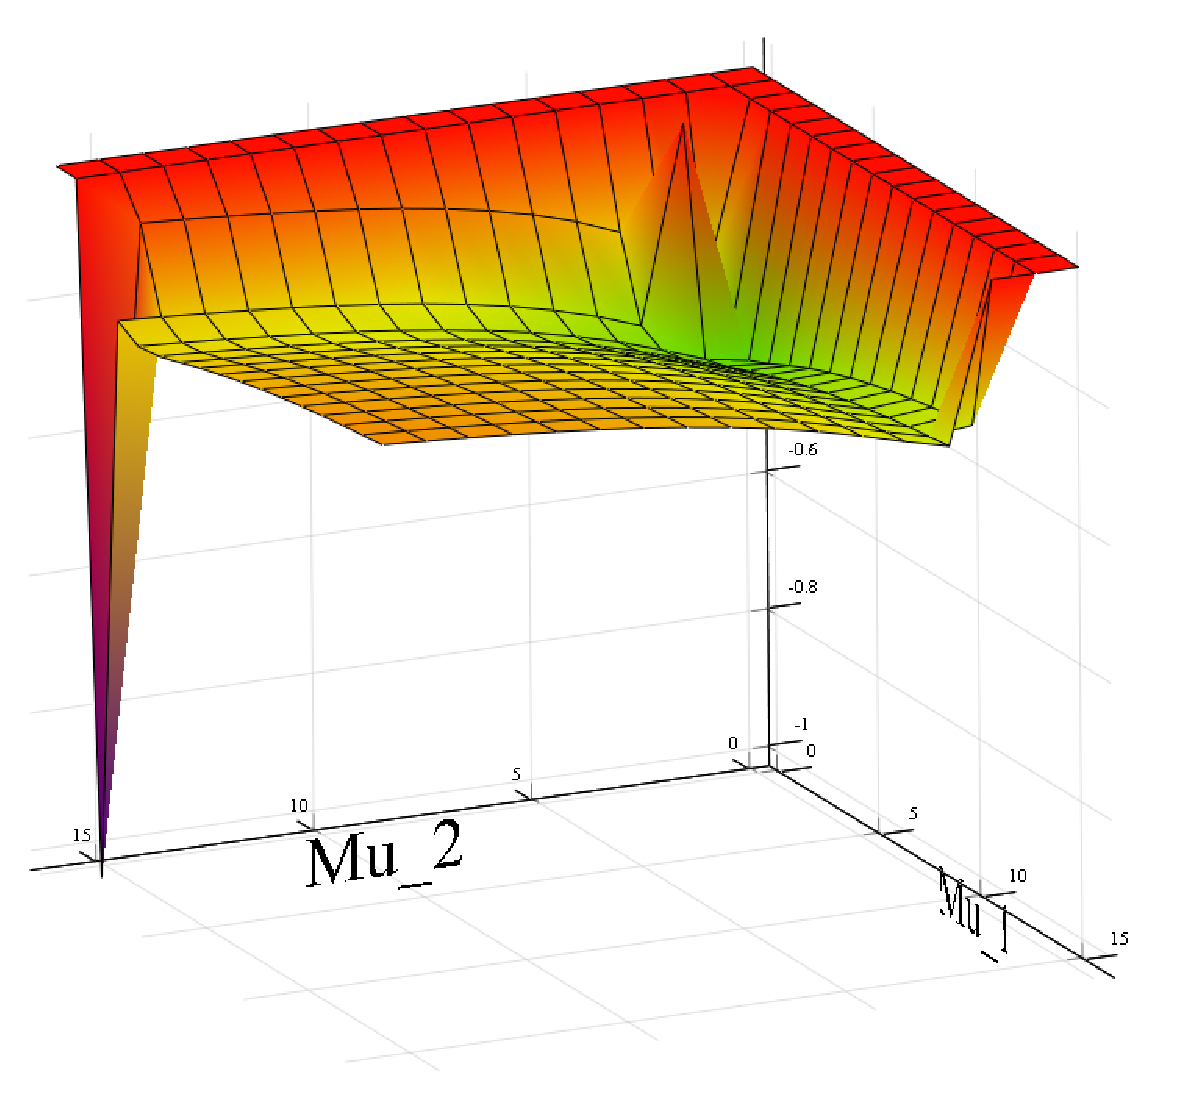
\includegraphics[scale=0.5]{corr_exp1.eps}
	\caption{Изменение корреляции при различных интенсивностях обслуживания}
	\label{exps_corr_exp1}
\end{figure} 

На рисунке \ref{exps_corr_exp1} представлено изменение коэффициента корреляции компонентов выходящего потока при варьировании $\mu_{1}$ и $\mu_{2}$. Коэффициент в выбранном диапазоне всегда имеет отрицательное значение, что означает снижение количества обслуженных заявок одного типа при увеличении другого. Также можно заметить, что при увеличении $\mu_{1}$ значение коэффициента корреляции ниже, чем при увеличении $\mu_{2}$. Это объясняется тем, что заявки входящего потока рано или поздно получать доступ к ресурсу, а их частое нахождение на приборе уменьшает время для поступления вызываемых заявок, которые при неудачной попытке поступления на прибор теряются.

Возьмем другую пару параметров для вариации: $\alpha,\lambda \in [2,16]$

\begin{figure}[H]
	\centering
	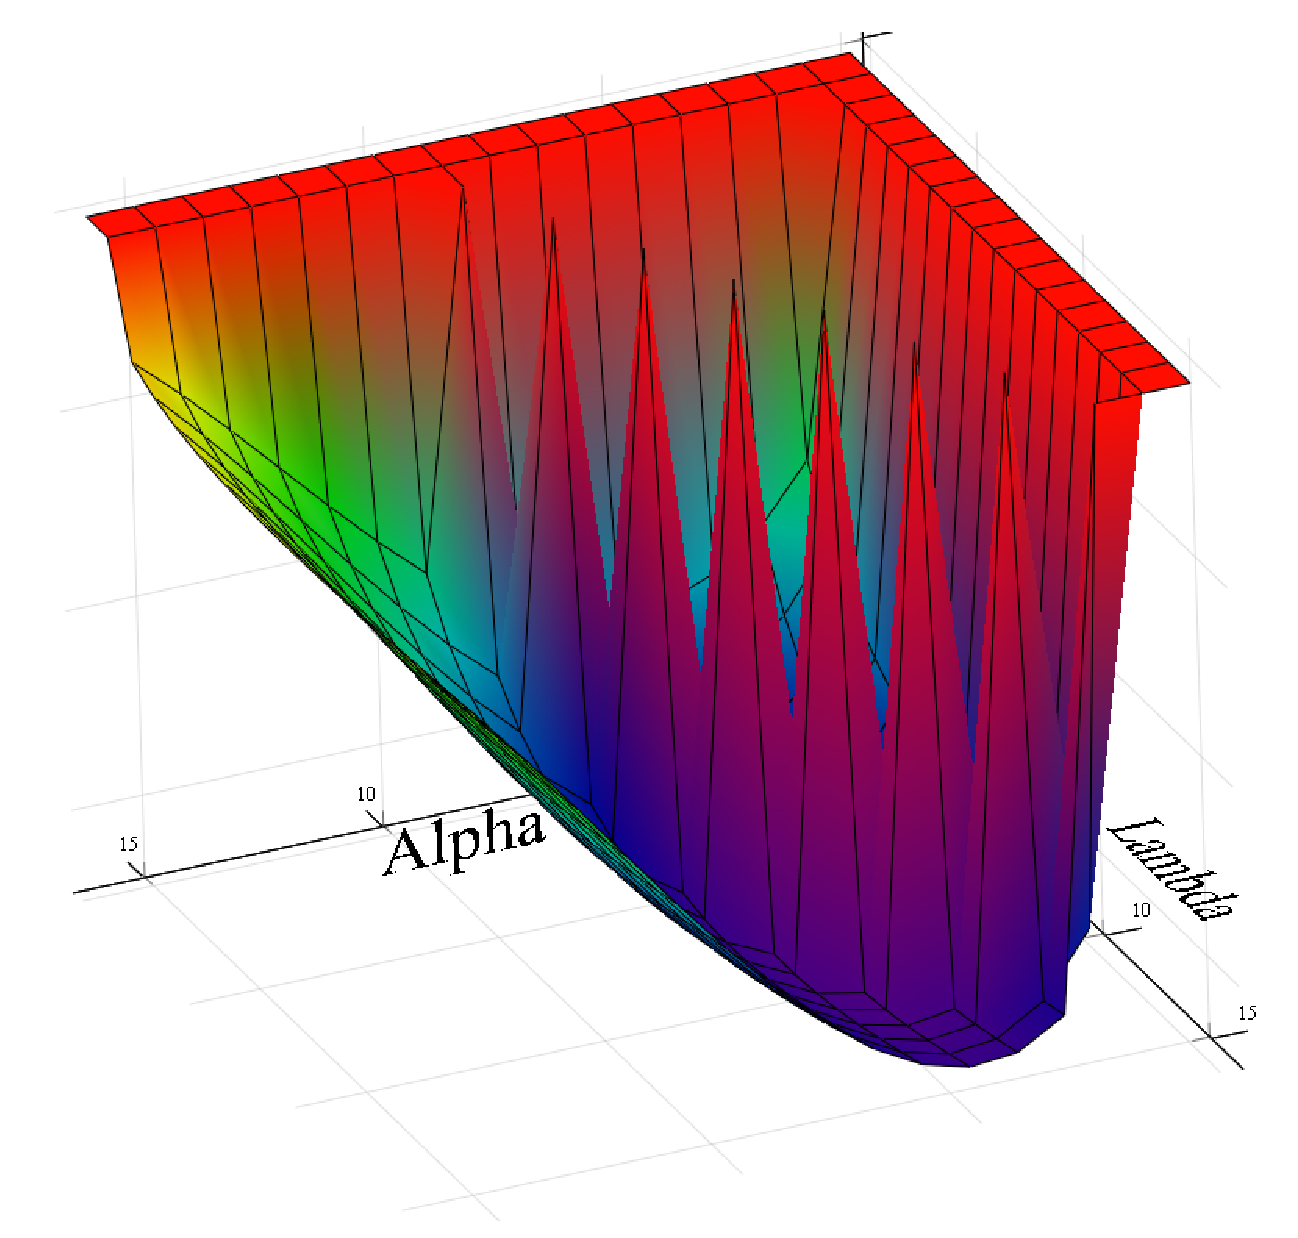
\includegraphics[scale=0.5]{corr_exp2.eps}
	\caption{Изменение корреляции при различных интенсивностях поступления заявок}
	\label{exps_corr_exp2}
\end{figure} 

Для данных параметров по сравнению с варьированием $\mu_{1}$ и $\mu_{2}$ наблюдается обратная тенденция --- при увеличении интенсивности поступления вызываемых заявок корреляция ниже, чем при более интенсивном входящем потоке заявок. Помимо этого, в результате проведенных расчетов были найдены параметры системы, при которых процессы обслуживания входящих заявок и вызываемых становятся независимыми. С данными параметрами с помощью имитационной модели было получено эмпирическое распределение вероятностей, на основе которого также была вычислена корреляция. Результаты совпадают, однако для подробного объяснения нулевого значения коэффициента корреляции при указанных параметрах требуется дальнейшее исследование в этом направлении.

Также стоит отметить, что при увеличении интенсивности входящего потока корреляция в целом стремится к нулю.

Расчеты для параметров: $\mu_{2},\lambda \in [2,16]$ и $\mu_{1},\alpha \in [2,16]$
\begin{figure}[H]
	\centering
	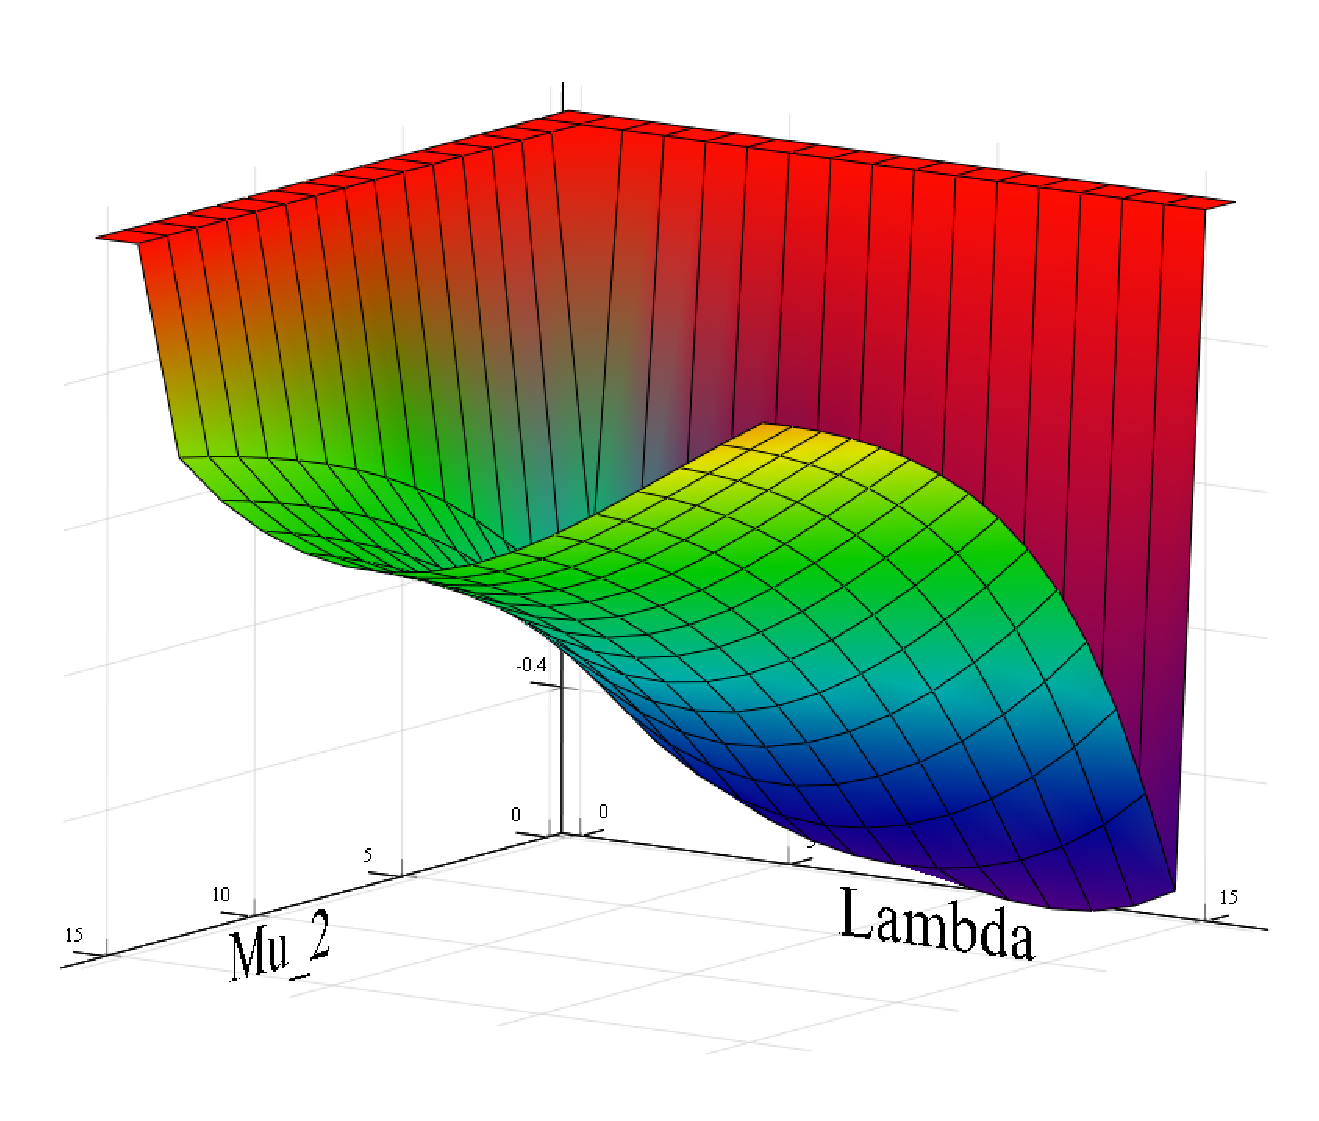
\includegraphics[scale=0.5]{corr_exp3.eps}
	\caption{Изменение корреляции при различных интенсивности обслуживания вызванных и интенсивности поступления заявок}
	\label{exps_corr_exp3}
\end{figure} 

\begin{figure}[H]
	\centering
	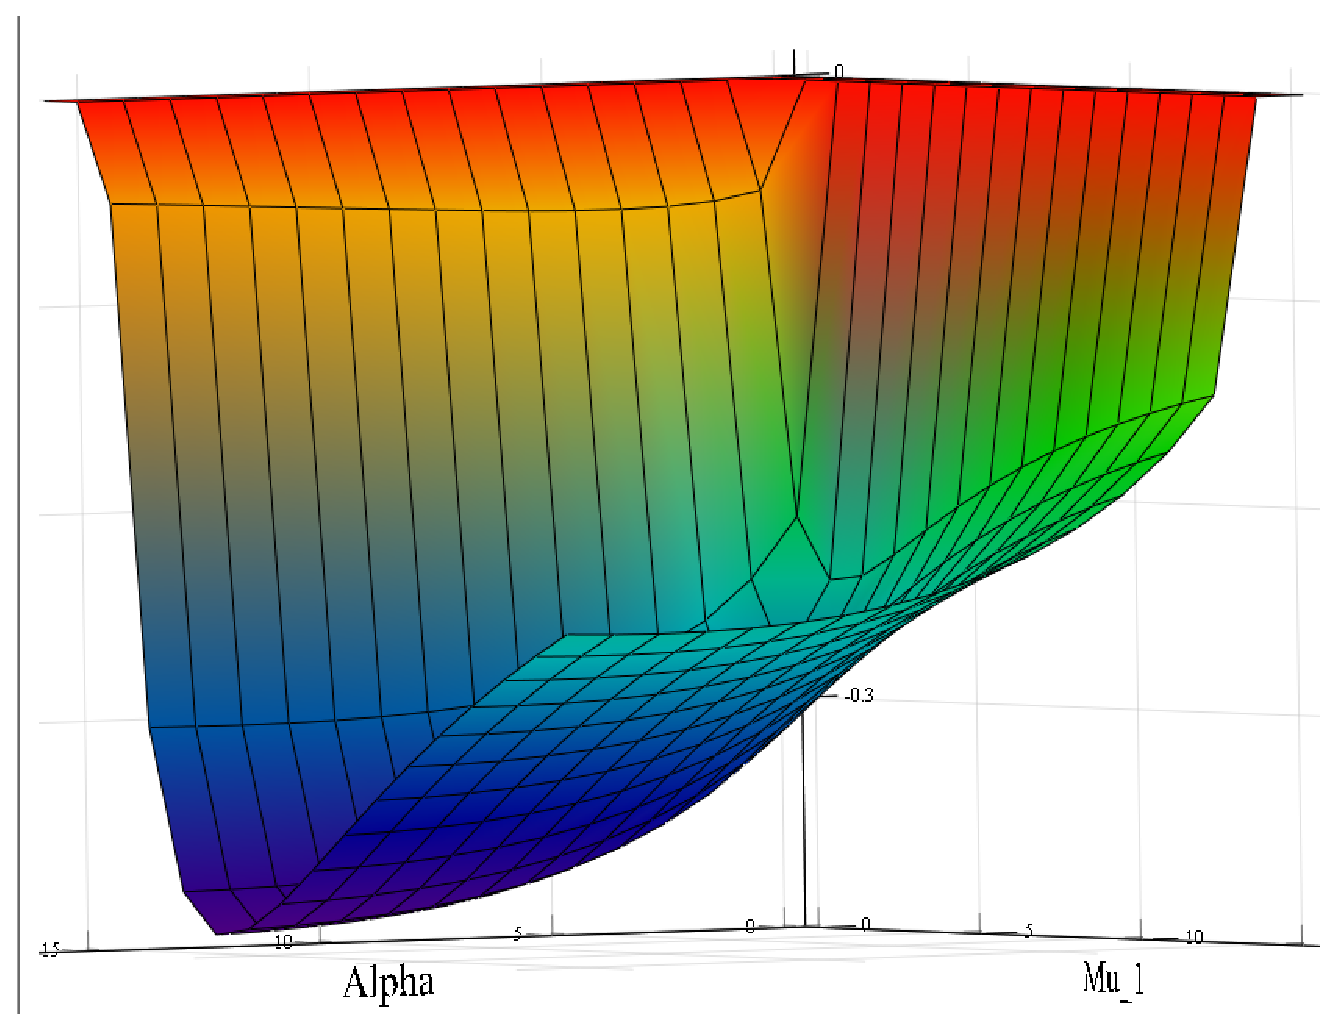
\includegraphics[scale=0.5]{corr_exp5.eps}
	\caption{Изменение корреляции при различных интенсивности обслуживания входящих и интенсивности вызова заявок}
	\label{exps_corr_exp5}
\end{figure} 

На рисунках \ref{exps_corr_exp3} и \ref{exps_corr_exp5} представлены расчеты коэффициента корреляции для интенсивностей поступления в систему одного типа заявок и интенсивности обслуживания другого. Расчеты представлена вместе, так как в них наблюдается закономерность --- при увеличении интенсивности поступления коэффициент корреляции принимает меньшие значения, а также он всегда отрицательный.

Теперь проведем расчеты для пар параметров одного типа заявок: $\mu_{2},\alpha \in [2,16]$ и $\mu_{1},\lambda \in [2,16]$
\begin{figure}[H]
	\centering
	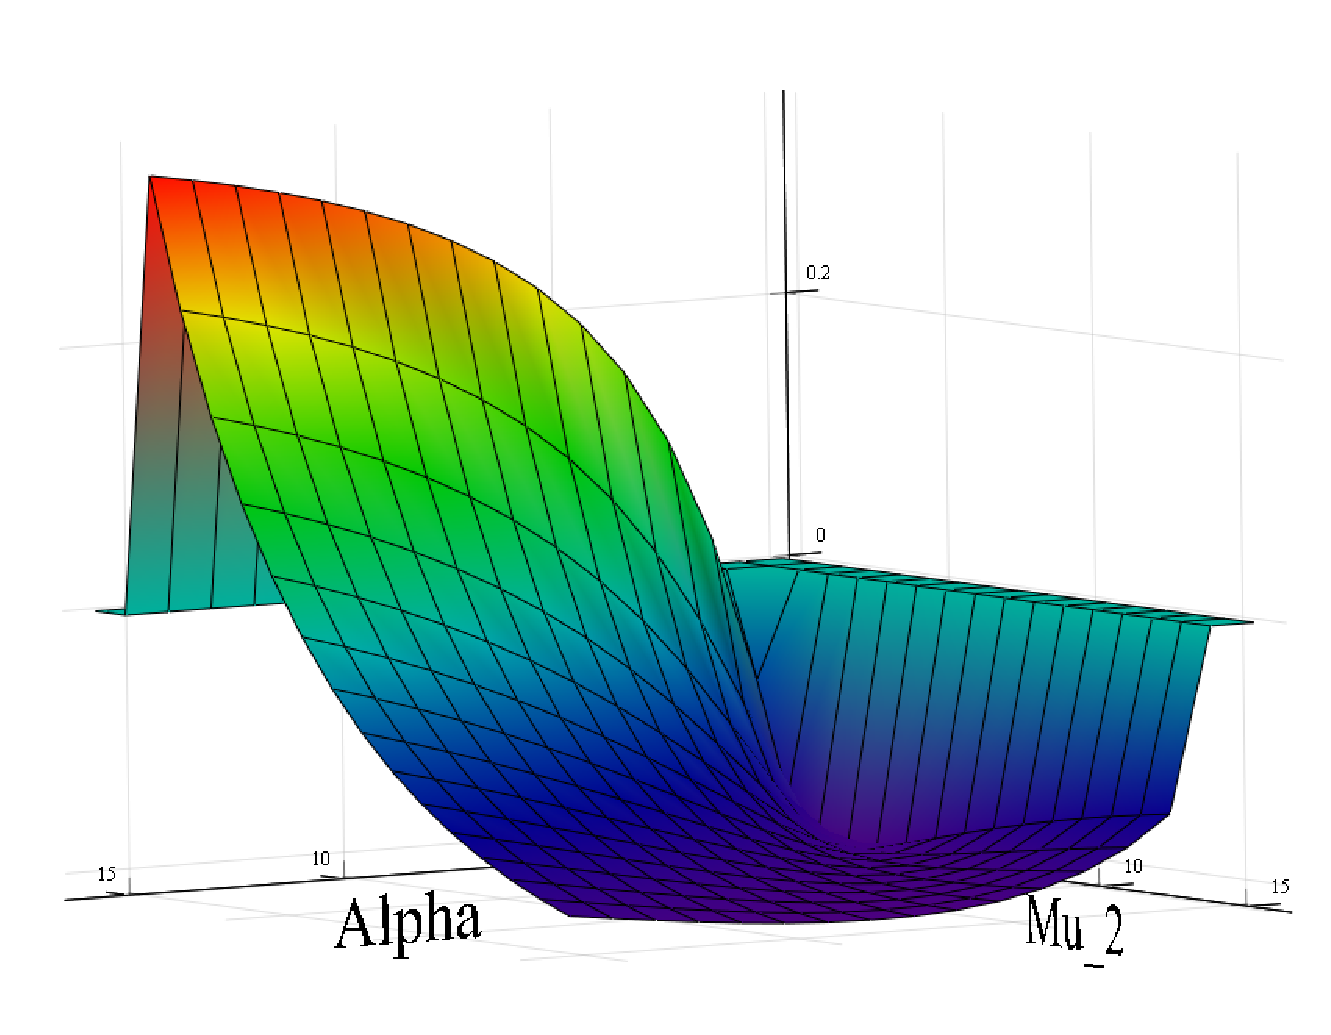
\includegraphics[scale=0.5]{corr_exp4.eps}
	\caption{Изменение корреляции при различных интенсивности обслуживания вызванных и интенсивности вызова заявок}
	\label{exps_corr_exp4}
\end{figure} 

\begin{figure}[H]
	\centering
	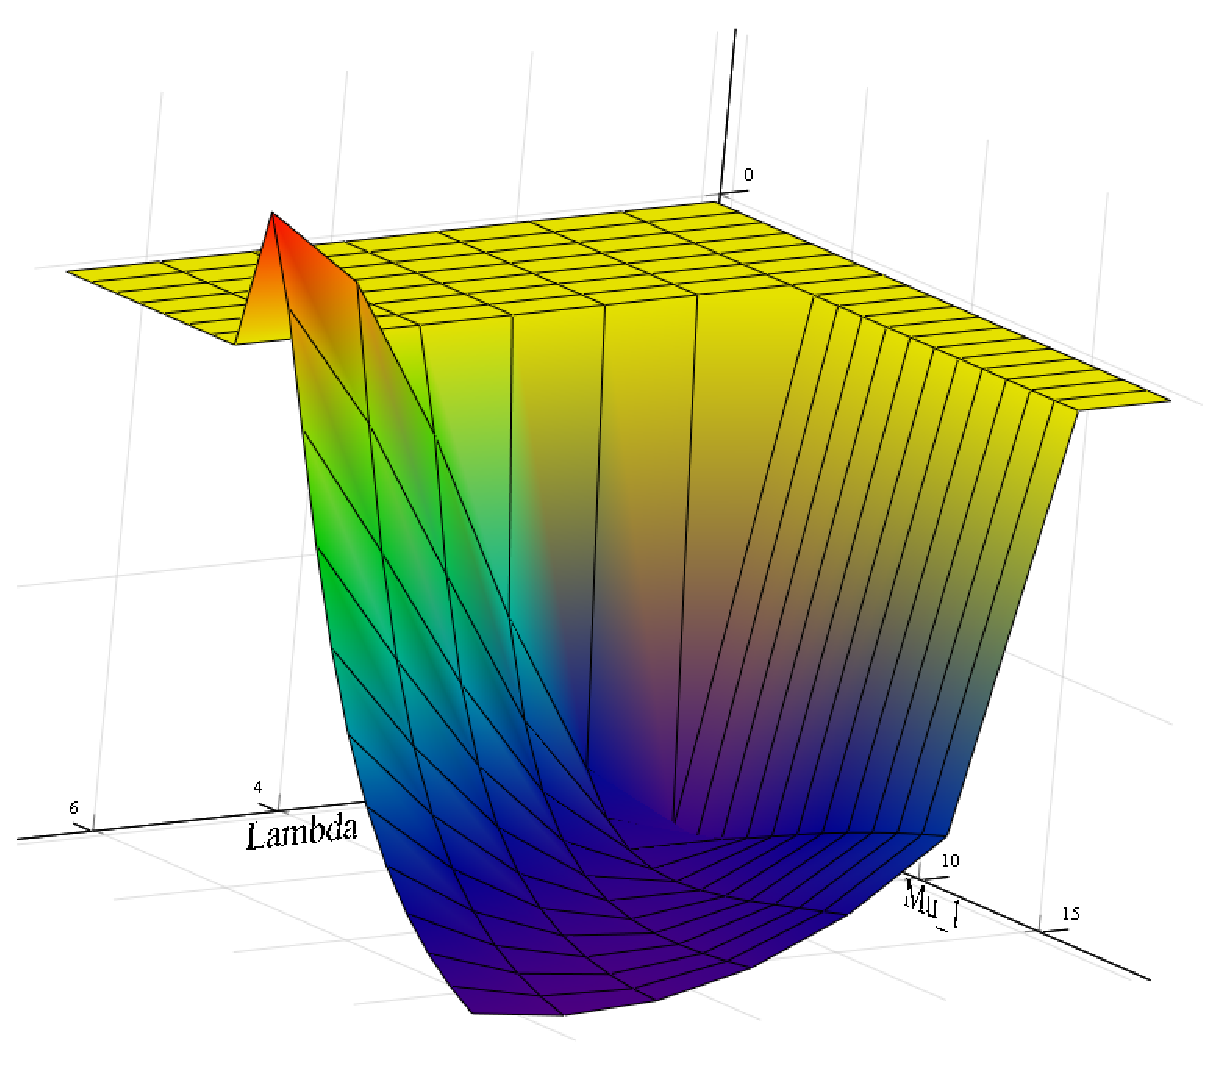
\includegraphics[scale=0.5]{corr_exp6.eps}
	\caption{Изменение корреляции при различных интенсивностях входящего потока и интенсивности обслуживания входящих заявок}
	\label{exps_corr_exp6}
\end{figure} 

При варьировании указанных наборов параметров на рисунках \ref{exps_corr_exp4} и \ref{exps_corr_exp6} видно, что коэффициент корреляции принимает как положительные, так и отрицательные значения.

Для RQ--системы с MMPP формула из раздела \ref{corr_section} не дает интерпретируемых результатов, поэтому для нее коэффициент корреляции был вычислен точечно при помощи распределения вероятностей, полученного в результаты имитационного моделирования при параметрах MMPP, соответствующих интенсивности простейшего входящего потока из экспериментов, описанных выше. Для этого была задана следующая матрица интенсивностей

 \begin{equation*}
	\boldsymbol{\Lambda}=\begin{bmatrix}
		1 &	0 & 0\\
		0 &	1 & 0\\
		0 &	0 & 1\\
	\end{bmatrix}.
\end{equation*}

При данной матрице $\Lambda$ общая интенсивность MMPP, вычисляемая, как $r\cdot Q\cdot E$ равна единице, как и интенсивность простейшего входящего потока в экспериментах с параметрами \eqref{simple_summary_input_params_corr}.

\begin{table}[htb!] 
	\centering
	\caption{Расчеты коэффициента корреляции для RQ--системы с MMPP}
	\label{corr_mmpp_table}
	\begin{tabular}{| c | c | c | c | c || c | c | c | c | c |}
		\hline
		$\mu_{2}$/$\mu_{1}$ & 2 & 4 & 6 & 8 & $\mu_{2}$/$\mu_{1}$ &  2 & 4 & 6 & 8\\ 
		\hline
		2 & -0.248 & -0.33 & -0.302 & -0.272 & 2 & -0.245 & -0.332 & -0.304 & -0.278 \\
		\hline
		4 & -0.171 & -0.3 & -0.282 & -0.263 & 4 & -0.168 & -0.301 & -0.285 & -0.264 \\
		\hline
		6 & -0.127 & -0.264 & -0.246 & -0.224 & 6 & -0.124 & -0.263 & -0.249 & -0.23\\
		\hline
		8 & -0.102 & -0.237 & -0.225 & -0.201 & 8 & -0.098 & -0.237 & -0.224 & -0.205\\
		\hline
	\end{tabular}
\end{table}

В таблице \ref{corr_mmpp_table} показаны результаты вычисления коэффициента корреляции для RQ--системы с MMPP--потоком с параметрами \eqref{simple_summary_input_params_corr} при помощи имитационного моделирования (слева) и результаты вычисления коэффициента корреляции для системы с простейшим потоком, графическое представление которых представлено на рисунке \ref{exps_corr_exp1} (cправа), при том условии, что интенсивности входящих потоков равны. Корреляция для системы с MMPP ввиду распределения вероятностей, полученного при моделировании, была вычислена с некоторой погрешностью, однако для соответствующих значений $\mu_{1}$ и $\mu_{2}$ коэффициенты приблизительно равны.

 %Численные эксперименты
\titleformat{\section}[block]
{\normalsize\bfseries\centering}
{\thesection}
{1em}{}
\section*{\centering\normalsize ЗАКЛЮЧЕНИЕ}
\addcontentsline{toc}{section}{Заключение}
В рамках данной работы был рассмотрен ряд методов оптимизации экспериментального исследования модели системы массового обслуживания с повторными вызовами и вызываемыми заявками. Согласно указанной цели исследования был выполнен ряд задач.

Была переработана имитационная модель с ориентацией на масштабные запуски и параллелизм. Была улучшена ее производительность и отказоустойчивость при задании параметров, затрудняющих процесс моделирования. Также была реализована возможность задания параметров для всех элементов системы из файла, который заранее содержит информацию о требуемых результатах.

Для работы с результатами моделирования были разработаны программные инструменты на языке Python, позволяющие генерировать необходимое количество наборов параметров, проводить множественные запуски имитационной модели и агрегировать полученные данные.

Помимо этого, в рамках программного комплекса были реализованы алгоритмы вычисления характеристик рассматриваемой модели системы массового обслуживания, включающие также вспомогательные функции для вычисления точности распределения вероятностей при помощи расстояния Колмогорова. Ключевой особенностью данного инструмента является наличие функций для подсчета распределения вероятностей при помощи дискретного преобразования Фурье. Их реализация позволяет существенно оптимизировать процесс проведения экспериментов, так как время работы алгоритмов во много раз превосходит ранее использованный подход.

В конечном итоге, разработанные инструменты позволили провести апробацию методов машинного обучения для расчета одной из характеристик работы системы --- вариации длин интервалов между моментами покидания заявками прибора. На основе выборки, составленной из 286 тысяч запусков имитационной модели, были обучены алгоритмы LinearRegression, RandomForest, GradientBoost и CatBoost для решения задачи регрессии. Были выявлены зависимости целевой переменной от ряда признаков, в частности, задержки заявок на орбите и коэффициента вариации входящего потока. Обученные модели позволяют получать результаты с достоверностью около 80\%. В дальнейшем исследовании стоит цель увеличить точность предсказаний за счет изменения процедуры генерации наборов параметров таким образом, чтобы распределение каждого признака было более равномерным и охватывало как можно большее количество возможных значений во избежание искажения результатов.

Часть результатов проведенного исследования были представлены в качестве докладов на двух международных конференциях:
\begin{itemize}
	\item XXIV International Conference on Distributed Computer and Communication Networks (DCCN) (сентябрь 2021, Томск) \cite{blaginin2021approximation};
	\item XX Международная конференции по информационным технологиям и математическому моделированию имени А.Ф. Терпугова (ITMM) (декабрь 2021, Томск);
\end{itemize}

 \clearpage %Заключение
\bibliographystyle{ugost2008mod}
\addcontentsline{toc}{section}{Список использованной литературы}
\bibliography{refs.bib}\nocite{*}
\clearpage
\includepdf[pagetemplate=1,scale=0.83,offset=0.75cm 0]{antiplagiat}
\end{document}